	\documentclass{DTEDI_KP}
	
\usepackage{longtable}

\usepackage[titles]{tocloft}
\renewcommand\cftfigpresnum{Gambar\ }
\renewcommand\cfttabpresnum{Tabel\  }

\usepackage{hyperref}
\newlength{\mylenf}
\settowidth{\mylenf}{\cftfigpresnum}
\setlength{\cftfignumwidth}{\dimexpr\mylenf+2em}
\setlength{\cfttabnumwidth}{\dimexpr\mylenf+2em}

\usepackage[labelfont=bf]{caption}

\usepackage{caption}
\usepackage{subcaption}
\usepackage{graphicx}
\usepackage{float}
\usepackage{textcomp}
\usepackage{amsmath}
%\usepackage{multirow}



\titleind{KINEMATIKA DAN ANTARMUKA ROBOT SCARA SERPENT}

\fullname {IVAN SYAHRONI HERMAWAN}

\idnum {17/415746/SV/13611}

\approvaldate {20 Januari 2020}

\degree {Teknologi Listrik}

\yearsubmit {2019}

\program {Teknologi Listrik}

\dept {Departemen Teknik Elektro dan Informatika}

\secondsupervisor {Fahmizal, S.T., M.Sc.}

\secondnip {111198807201609101}

\firstsupervisor {Ma’un Budiyanto,  S.T., M.T.}

\firstnip {197007071999031002}

\begin{document}
	
	\cover
	
	\approvalpage
	
	\preface
	
Puji syukur penulis panjatkan kehadirat Tuhan Yang Maha Esa karena hanya dengan rahmat dan hidayah-Nya, laporan kerja praktik ini dapat diselesaikan tanpa halangan yang berarti. Keberhasilan dalam menyusun laporan kerja praktik ini tidak lepas dari bantuan berbagai pihak yang mana dengan tulus dan ikhlas membe- rikan masukan guna sempurnanya laporan kerja praktik ini.  Oleh karena itu dalam kesempatan ini, dengan kerendahan hati penulis mengucap terima kasih kepada:
	
	\begin{enumerate}
		\item Bapak Ma’un Budiyanto, S.T., M.T. selaku Ketua Program Studi Teknologi Listrik Universitas Gadjah Mada,
		\item  Bapak Fahmizal, S.T., M.Sc selaku dosen pembimbing pertama yang telah memberikan banyak bantuan, bimbingan, serta arahan dalam kerja praktik,
		\item Seluruh Dosen di Teknologi Listrik Sekolah Vokasi Universitas Gadjah Mada, yang tidak bisa disebutkan satu-satu, atas ilmu dan bimbingannya,
		\item Sugeng Julianto S.ST, selaku laboran yang memfasilitasi Labolatorium Instrumentasi dan Kendali sehingga tugas akhir penulis berjalan dengan baik, 
		\item Teman – teman Lab Kendali, Tirza, Mas Galih, Mas Ma'ruf, Mas Bayu, Fajar, Denny dan lain – lain yang selalu memberi semangat, inspirasi, dukungan serta bantuanya pada penulis dalam mengerjakan kerja praktik,
		\item Ibu dan Bapak yang selama ini telah sabar membimbing, mengarahkan, dan mendoakan penulis tanpa kenal lelah untuk selama-lamanya.
		
	\end{enumerate}

Penulis menyadari bahwa penyusunan laporan kerja praktik ini jauh dari sempurna. Kritik dan saran dapat ditujukan langsung pada e-\textit{mail} saya. Akhir kata penulis mohon maaf yang sebesar-besarnya apabila terdapat kekeliruan di dalam penulisan kerja praktik ini.

\vspace{0.1cm}

	\begin{tabular}{p{7.5cm}c}
	&Yogyakarta, 20 Februari 2020 \\\
	&\\
	&\\
	&\\
	&\\
	&\textbf{Penulis}
	\end{tabular}

\tableofcontents
\addcontentsline{toc}{chapter}{DAFTAR ISI}
\listoftables
\addcontentsline{toc}{chapter}{DAFTAR TABEL}
\listoffigures
\addcontentsline{toc}{chapter}{DAFTAR GAMBAR}

\begin{abstractind}
	Makalah ini menyajikan kendali pergerakan posisi dari robot SCARA Serpent menggunakan persamaan kinematika serta perancangan desain antarmuka menggunakan Processing IDE. Antarmuka bertujuan untuk memudahkan pengguna dalam mengendalikan dan mendapatkan data berupa koordinat objek yang nantinya koordinat objek tersebut digunakan sebagai masukan untuk kinematika balik. Umpan balik yang digunakan dalam robot SCARA Serpent merupakan sensor potensiometer yang ditempatkan pada masing-masing \textit{joint}. Selain itu, untuk mendapatkan hasil pergerakan robot yang baik pada sistem kinematika, kendali PID diterapkan untuk mengendalikan kecepatan putar setiap motor DC pada setiap \textit{joint} untuk mencapai sebuah posisi. Untuk menguji ketepatan posisi dari kinerja sistem kinematika robot SCARA Serpent, terdapat lima jenis pengujian, yaitu pengujian koordinat $x$, pengujian koordinat $y$, pengujian sudut \textit{shoulder}, pengujian sudut \textit{elbow}, pengujian sistem secara keseluruhan dan pengujian dengan kendali proposional. Dari hasil tes ini sistem dapat berjalan dengan baik dengan nilai \textit{error} di bawah 5\% menggunakan kendali Kp 0,2 Ki ...
	
	
	\textbf{Kata kunci }: SCARA Serpent, \textit{Arm Robot Manipulator}, Kinematika, Processing IDE, \textit{Invers Kinematic}.
\end{abstractind}

\begin{abstracteng}
	\textit{This paper presents the position movement control of the SCARA Serpent robot using kinematics equations and interface design using the Processing IDE. The interface aims to make it easier for users to control and obtain data in the form of object coordinates which will later be used as input for back kinematics. The feedback used in the SCARA Serpent robot is a potentiometer sensor placed at each joint. In addition, to get good robot movement results on the kinematics system, PID control is applied to control the rotational speed of each DC motor in each joint to reach a position. To test the accuracy of the position of the SCARA Serpent robot kinematics system performance, there are five types of testing, namely $x$ coordinate testing, $y$ coordinate testing, shoulder angle testing, elbow angle testing, overall system testing and proportional control testing. From the results of this test the system can run well with an error value below 5 \% using the Kp control of 0.2 Ki ...}
	
	
	\textit{\textbf{Keyword}} : SCARA Serpent, \textit{Arm Robot Manipulator}, \textit{kinematics}, Processing IDE, \textit{Invers Kinematic}.
\end{abstracteng}

\newpage
\setcounter{page}{1}
\pagenumbering{arabic}

%BAB-1 Laporan KP

\chapter{PENDAHULUAN}

\section{Latar Belakang Masalah}

Perkembangan teknologi serta ilmu pengetahuan pada masa ke masa semakin berkembang. Perkembangan ini berjalan seiring dengan penelitian-penelitian di berbagai disiplin ilmu khususnya dalam bidang instrumentasi dan kendali. Hal ini dapat dilihat dari banyaknya penggunaan sistem instrumentasi dan kendali dalam dunia industri seperti pengguanaan robot dalam menyelesaikan pekerjaan manusia. Untuk itu perancangan robot merupakan salah satu solusi untuk memenuhi tuntutan dalam membantu kebutuhan manusia \cite{Faris2012}.

Pemilihan robot untuk menggantikan pekerjaan manusia tidak terlepas dengan berbagai kelebihannya. Salah satu kelebihannya, sebuah robot dapat melakukan suatu pekerjaan yang sama dan berulang tanpa merasakan lelah seperti halnya manusia. Pekerjaan ini lah yang biasa ditemukan dalam bidang industri khususnya pada bagian produksi. Robot dengan sistem lengan robot (\emph {robot arm system}) merupakan salah satu jenis robot yang dominan berada dalam bidang industri\cite{Bimantaka2014}. 

Salah satu dari jenis dari robot lengan adalah\textit{ selective compilance assembly robot arm} atau biasa dikenal dengan robot SCARA Serpent. Robot SCARA Serpent terdiri dari \textit{base}, lengan \textit{shoulder}, \textit{elbow} dan \textit{end-effector}. Posisi \textit{end-effector} pada robot SCARA Serpent berada pada sebuah koordiant kartesian ($x, y$). Nilai koordinat ($x, y$) diubah menjadi sebuah nilai sudut yang digunakan untuk lengan \textit{shoulder} dan \textit{elbow} dengan menggunakan sebuah persamaan kinematika balik.  

Pada laporan penelitian kerja praktik ini lebih difokuskan terhadap gerak kinematika dari robot serta perancangan antarmuka untuk memudahkan dalam mengoperasikan robot. Robot SCARA Serpent telah banyak dijadikan sebagai objek penelitian, salah satu penelitian robot SCARA Serpent Serpent yang populer merupakan penelitian tentang menjadikan robot SCARA Serpent menjadi robot yang dapat memindahkan objek tergantung warna dari masing-masing objek. Dengan penelitian tersebut maka robot SCARA Serpent dapat memiliki fungsi lebih banyak serta dapat ditempatkan ke dalam dunia industri.

Dalam berbagai penelitian tentang robot SCARA Serpent, banyak ditemukan beberapa masalah yang sering terjadi terkait robot SCARA Serpent. Masalah yang umum terjadi adalah terbatasnya pergerakan pada garis vertikal. Robot SCARA Serpent dalam melakukan pergerakan vertikal dijalankan menggunakan \textit{joint prismatic} yang terletak pada \textit{end effector}. Dengan begitu pergerakan vertikal dalam robot dibatasi oleh minimnya panjang \textit{link} pada \textit{end-effector} yang menyebabkan objek yang dapat diambil oleh robot SCARA Serpent tidak dapat terlalu tinggi.

Dalam mengendalikan sebuah robot dibutuhkan \textit{platfrom} antarmuka sebagai jembatan antara \textit{user} dengan \emph{hardware}. Dalam penelitian ini program antarmuka dirancang menggunakan \textit{software} Processing IDE. Penggunaan Processing IDE sebagai antarmuka karena memiliki beberapa keunggulan, seperti mudahnya sarana komunikasi terhadap \emph {hardware} yang digunakan. Oleh karena itu, pada program kerja praktik ini dilakukan analisis kinematika robot SCARA Serpent dengan perancangan antarmuka berbasis  Processing IDE.\\


\section{Tujuan Penelitian}
Adapun tujuan dalam melaksanakan penelitian "Kinematika dan Antarmuka Robot SCARA Serpent" adalah sebagai berikut:

\subsection{Secara Umum}
\begin{enumerate}
	\item Merancang\emph{ arm manipulator robot} SCARA Serpent berbasis Arduino Mega 2560.
	\item Memahami dan mengimplementasikan antarmuka Processing \textit{integrated development environment} (IDE).
	\item Mengimplementasikan kinematika pada \emph{arm manipulator robot} SCARA Serpent.
\end{enumerate}
\subsection{Tujuan Khusus}
Untuk memenuhi salah satu syarat kelulusan dalam menempuh pendidikan Program   Diploma III Teknologi Listrik, Sekolah Vokasi, Universitas Gadjah Mada. 


\section{Batasan Penelitian}
Pembatasan masalah diperlukan untuk mempermudah pelaksanaan penulisan laporan kerja praktik sehingga tidak menyimpang dari judul laporan. Lingkup pembatasan masalah dalam laporan kerja praktik ini dibatasi pada:

\begin{enumerate}
	
	\item Akurasi dari robot lengan dipengaruhi oleh spesifikasi dan torsi dari masing-masing motor DC pada \emph{ joint.}
	\item  Rancangan mekanik yang sudah tersusun dari awal sehingga tidak dapat diubah lagi. 
	\item Besar objek yang dapat dibawa oleh \textit{gripper} memiliki ukuran yang terbatas.
	\item Komunikasi antara Processing IDE dan \textit{hardware} menggunakan komunikasi serial yang dihubungkan dengan kabel USB.
	
\end{enumerate}

\section{Metode Kerja Praktik}
Metodologi adalah suatu cara yang digunakan untuk memperoleh data yang akurat, baik melalui observasi lapangan maupun dari \emph {datasheet} setiap alat yang digunakan. Observasi juga dilakukan dengan meninjau jurnal-jurnal dan konsultasi mengenai penelitian yang dilakukan. Pada bagian ini dijelaskan meliputi waktu dan tempat penelitian, alat dan bahan penelitian, rancangan alat, metode penelitian dan prosedur penelitian. Penjelasan lebih rinci tentang metodologi penelitian akan dijelaskan sebagai berikut: 

\begin{enumerate}
	\item Waktu dan Tempat Penelitian \\
	Penelitian dilakukan di Labolatorium Instrumentasi dan Kendali Departemen Teknik Elektro dan Informatika (DTEDI) Sekolah Vokasi Universitas Gadjah Mada pada bulan Juli sampai bulan Agustus 2019.
	
	\item Alat dan Bahan \\
	Peralatan yang digunakan dalam kerja praktik adalah personal \textit{computer} (PC), Arduino Mega 2560, transformator AC 5A, \textit{converter} AC to DC, modul DC to DC \textit{converter} LM2596, IC TIP 31, multimeter,\textit{ valve pneumatic}, \textit{driver} motor EMS 30A dan catu daya AC 220 Volt. Sedangkan bahan yang digunakan adalah motor DC yang terpasang di setiap \emph {joint} robot lengan serta \textit{valve relay pneumatic} untuk mengkontrol tekananan udara.
	
	\item  Pengumpulan Data \\
	Studi pustaka dilakukan dengan cara mengumpulkan buku-buku, dokumen, serta jurnal-jurnal berbentuk \emph{e-book} yang berkaitan dengan robot lengan. Selain itu \emph{datasheet} dari setiap komponen juga ditinjau. Data-data tersebut menjadi referensi untuk merancang, membuat, dan menguji alat. 
	
	Konsultasi dilakukan untuk mengumpulkan data melalui tanya jawab atau berdiskusi dengan pihak yang mengetahui dan menguasai segala permasalahan yang dihadapi dalam merancang, membuat, dan menguji robot lengan SCARA Serpent. Dalam metode ini penulis berdiskusi dengan dosen pembimbing kerja praktik. 
	
	\item Metode Penelitian \\
	Metode penelitian yang dilakukan meliputi; pengujian tegangan DC to DC \textit{converter}, pengujian motor DC, pengujian \textit{driver} motor DC EMS 30A, pengujian rangkaian \textit{switching valve pneumatic}, pengujian kinematika balik, pengujian dengan kendali proposional serta pengambilan data dan analisa data.
	
	\item Prosedur Penelitian\\
	Prosedur penelitian adalah langkah-langkah dalam menyelesaikan kerja praktik yang akan disajikan dalam bentuk diagram alir pada Gambar \ref{pic.diagramalir}.
	
	\begin{figure}[H]
		\centering
		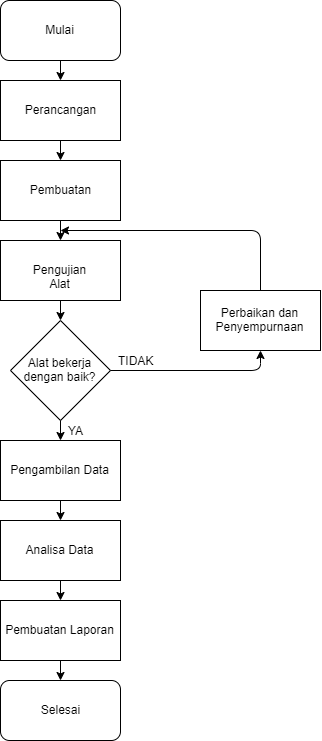
\includegraphics[width=7cm]{gambar/flowchart.png}
		\caption{ Diagram Alir Prosedur Penelitian}
		\label{pic.diagramalir}
	\end{figure}
	
	
\end{enumerate}

\section{Sistematika Penulisan}
Penulisan laporan kerja praktik ini dilakukan dengan mengikuti sistematika sebagai berikut:\\
\noindent
\textbf{BAB I\hspace*{0.6cm} PENDAHULUAN}\\
\noindent
Merupakan pendahuluan dari laporan kerja praktik yang menjelaskan latar belakang, tujuan, batasan masalah dan metodologi penyusunan laporan kerja praktik.\\
\noindent
\textbf{BAB II\hspace*{0.5cm} LANDASAN TEORI}\\
\noindent
Memuat gambaran umum robot lengan, \emph {degress of freedom}, konfigurasi robot lengan, \emph{wrist} dan \textit{end-effector}, kinematika, pengertian dan prinsip kerja Processing IDE sebagai antarmuka robot lengan, dan prinsip kerja setiap piranti yang digunakan dalam pembuatan robot lengan. \\
\textbf{BAB III\hspace*{0.375cm}  PERANCANGAN SISTEM}\\
\noindent
Memuat perancangan sistem secara umum, perancangan perangkat keras berupa elektronis dari robot lengan, perancangan perangkat lunak berupa pengolahan \textit{graphical user interface} (GUI) menggunakan Processing IDE, sistem kinematika balik untuk robot lengan, dan integrasi keseluruhan program. \\
\textbf{BAB IV\hspace*{0.4cm}  PENGUJIAN DAN ANALISA KERJA SISTEM }\\
\noindent
Memuat pengujian tegangan DC to DC \textit{converter}, pengujian motor DC, pengujian \textit{driver} motor DC EMS 30A, pengujian rangkaian \textit{switching valve pneumatic}, pengujian kinematika balik, pengujian dengan kendali proposional, serta pengambilan data dan analisa data hingga pada pengujian menyeluruh.\\
\textbf{BAB V\hspace*{0.6cm} PENUTUP}\\
Memuat tentang kesimpulan dari perancangan, pengujian dan analisis dari sistem kerja robot, serta berisi saran – saran untuk mengembangkan penelitian \emph{ arm manipulator robot} SCARA Serpent lebih lanjut. \\
%BAB_2 LAPORAN KP
\chapter{LANDASAN TEORI}

\section{Gambaran Umum Robot Lengan}

Robot adalah adalah sebuah alat yang terdiri dari gabungan mekanik dan elektronik yang dapat melakukan tugas fisik, baik menggunakan pengawasan, kendali manusia maupun secara otomatis. Robot dapat melakukan suatu tugas secara berulang tanpa merasa lelah sehingga robot banyak digunakan dalam dunia industri khususnya pada bidang produksi. Salah satu jenis robot yang sering digunakan dalam bidang produksi adalah sistem lengan robot\cite{Pandu}.

Robot lengan adalah robot yang memiliki bentuk fisik seperti halnya lengan pada manusia dan memiliki derajat kebebasan (\emph{degre of freedom}) tertentu bergantung pada jumlah sendi yang digunakan. Robot lengan pada bidang industri biasa digunakan sebagai aktuator untuk mengambil dan meletakkan suatu objek secara terus menerus.


Pada umumnya struktur robot lengan terdiri dari beberapa bagian.  Bagian utama dari robot lengan adalah struktur mekanik ({\textit{manipulator}}) yang merupakan susunan kerangka yang tidak dapat digerakkan (\emph{rigid}) dan lengan (\emph{link}) yang satu sama lain terhubung oleh sendi (\emph {joint}). Dengan adanya \emph{joint} yang menghubungkan dua \emph{link} menjadi satu kesatuan sehingga \emph{joint} membentuk satu derajat kebebasan. Jika diibaratkan dengan tubuh manusia, \emph{link} adalah tulang sedangkan \emph{joint} adalah sendi-sendinya. \emph{Joint} memiliki dua pergerakan, yaitu pergerakan \emph{revolute joint} (gerak berputar) dan \emph{prismatic joint} (gerak bergeser)\cite{mahmud2012}. Jenis-jenis \textit{joint} ditnjukkan pada Gambar \ref{pic.jenisjoint}.

\begin{figure}[H]
	\centering
	\includegraphics[width=11cm]{gambar/joint.png}
	\caption{Jenis-Jenis \textit{Joint}}
	\label{pic.jenisjoint}
\end{figure}


\subsection{\emph{Degress of Freedom }}
\emph{Degress of freedom} (DOF) merupakan sebuah konfigurasi yang dapat meminimalkan spesifikasi dengan menggunakan parameter yang dapat menyatakan posisi suatu sistem pada setiap saat. Umumnya robot lengan mempunyai paling sedikit enam independen derajat kebebasan, tiga derajat kebebasan untuk translasi dan tiga derajat kebebasan untuk rotasi. Namun, robot lengan paling tidak memiliki tiga derajat kebebasan untuk dapat memiliki \emph{workspace} yang cukup. \emph{Workspace} dari sebuah robot lengan merupakan total volume yang dapat dijangkau oleh \emph{end-effector} dari pergerakan semua \emph{joint}-nya dari titik minimum hingga maksimum\cite{Spong2006}. 

\subsection{Konfigurasi Robot Lengan}
Pada dasarnya berbagai jenis dari robot lengan dapat dibedakan dari konfigurasinya. Konfigurasi robot lengan merupakan perpaduan antara pergerakan \emph{joint} yang dimiliki oleh robot lengan. Konfigurasi ini memiliki tipe yang berbeda-beda sehingga \emph {workspace} yang dimiliki pada tiap robot lengan pasti berbeda.

\subsubsection{Konfigurasi \emph{Articulated} (\emph{Revolute - Revolute - Revolute)}} 
\emph{Articulated} manipulator ini pada dasarnya mempunyai jenis \emph{revolute joint} pada ketiga \emph{joint} robot lengan (\emph {base, shoulder, elbow}). Dengan konfigurasi ini, robot lengan dengan konfigurasi \textit{articulated} dapat memiliki variasi DOF yang banyak. DOF yang dapat dihasilkan dengan robot lengan dengan konfigurasi seperti ini adalah tiga DOF hingga sampai dengan enam DOF tergantung dari kebutuhan dan fungsi yang akan dilakukan oleh robot lengan. Konfigurasi dari \textit{joint revolute} ini menjadikan robot lengan jenis ini mempunyai kebebasan yang besar dari pergerakannya dalam ruang yang kecil sehingga menjadikan jenis konfigurasi \textit{articulated} manipulator ini banyak dipakai dan memiki desain yang populer. Konfigurasi dari \textit{articulated} ditunjukkan pada Gambar \ref{pic.articulated}. 
\begin{figure}[H]
	\centering
	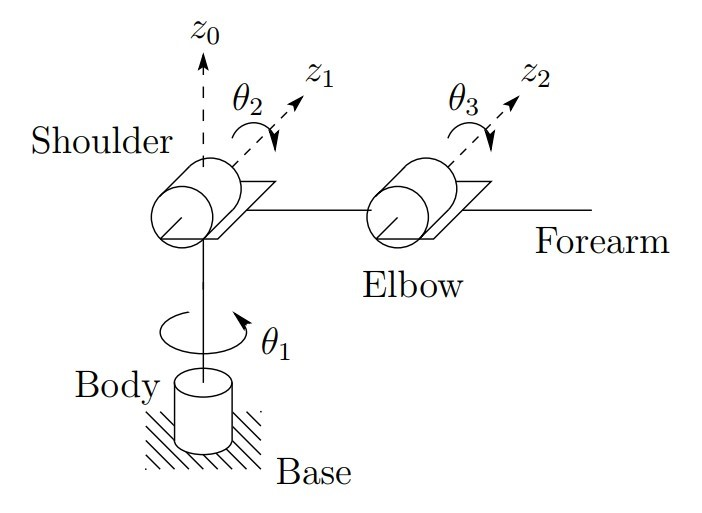
\includegraphics[width=8cm]{gambar/articulated.jpg}
	\caption{Struktur dari Konfigurasi  \textit{Articulated}\cite{Spong2006}}
	\label{pic.articulated}
\end{figure}
\subsubsection{Konfigurasi \textit{Spherical} (\textit{Revolute – Revolute – Prismatic})} 

Konfigurasi \textit{spherical} merupakan konfigurasi yang mempunyai dua buah \textit{joint revolute} dan satu buah \textit{joint prismatic}. \textit{Joint prismatic} berada ini \textit{joint} ketiga atau pada bagian \textit{elbow}. Sementara dua \textit{joint} lainnya berada di \textit{shoulder} dan \textit{wrist}. Struktur dari konfigurasi \textit{spherical} ditunjukkan pada Gambar \ref{pic.spherical}. 
\begin{figure}[H]
	\centering
	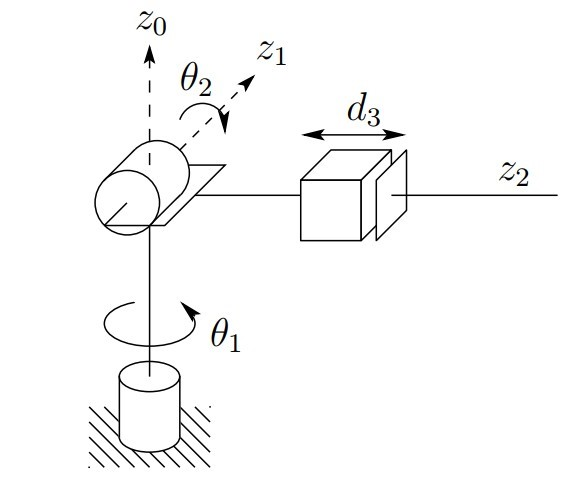
\includegraphics[width=8cm]{gambar/spherical.jpg}
	\caption{Struktur dari Konfigurasi \textit{Sperical}\cite{Spong2006}}
	\label{pic.spherical}
\end{figure}


\subsubsection{Konfigurasi SCARA Serpent Serpent (\textit{Revolute – Revolute – Prismatic}) } 

Konfigurasi \textit{selective compliant articulated robot for assembly} (SCARA Serpent) merupakan konfigurasi yang mempunyai dua buah \textit{joint revolute} dan satu buah \textit{joint prismatic} sama seperti konfigurasi \textit{spherical}. Meskipun SCARA Serpent memiliki struktur \textit{joint revolute – revolute – prismatic} (RRP) sama seperti konfigurasi yang dimiliki \textit{spherical}, struktur ini sedikit berbeda dengan konfigurasi \textit{spherical} dari tampilannya maupun dari jarak \textit{workspace} nya. Konfigurasi SCARA Serpent memiliki $z_{0}$ tegak lurus terhadap $z_{1}$, dan $z_{1}$ tegak lurus dengan $z_{2}$, konfigurasi SCARA Serpent memiliki struktur $z_{0}, z_{1}, dan z_{2}$ yang paralel. Struktur dan konfigurasi dari SCARA Serpent ditunjukkan pada Gambar \ref{pic.SCARA}.
\begin{figure}[H]
	\centering
	\label{pic.SCARA}
	\includegraphics[width=8cm]{gambar/SCARA.jpg}
	\caption{Struktur dari Konfigurasi SCARA Serpent\cite{Spong2006}}
	
\end{figure}


\subsubsection{Konfigurasi \textit{Cartesian} (\textit{Prismatic – Prismatic – Prismatic})  } 

Konfigurasi \textit{cartesian} mempunyai tiga buah \textit{joint prismatic}. Variabel \textit{joint} dari konfigurasi \textit{prismatic} adalah koordinat \textit{cartesian} dari \textit{end-effector} dengan memperhatikan letak \textit{base} dari robot lengan. Kinematika dari jenis konfigurasi ini adalah yang paling sederhana dari semua konfigurasi robot lengan. Konfigurasi \textit{cartesian} sangat berguna untuk penyusunan suatu barang di bidang datar seperti mesin laser, kargo atau memindahkan barang. Struktur dari konfigurasi \textit{cartesian} ditunjukkan pada Gambar \ref{pic.cartesian}.

\begin{figure}[H]
	\centering
	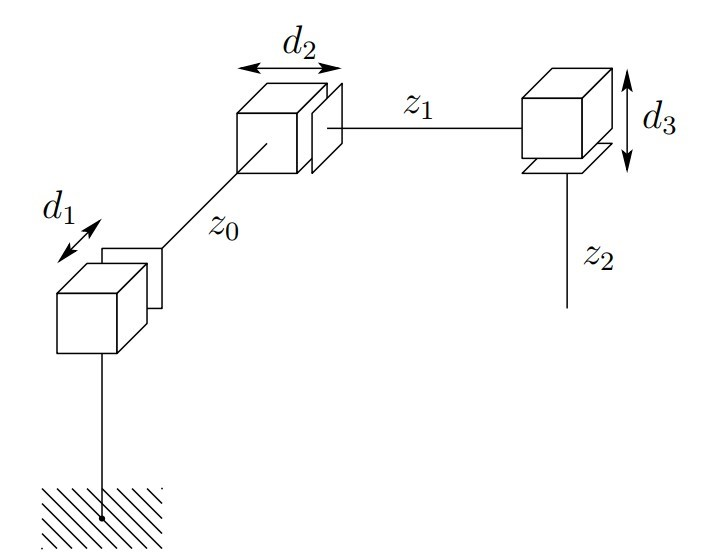
\includegraphics[width=6cm]{gambar/cartesian.jpg}
	\caption{Struktur dari Konfigurasi \textit{Cartesian}\cite{Spong2006}}
	\label{pic.cartesian}
\end{figure}

\subsection{ \textit{Wrist} dan \textit{End-effector} }

\textit{Wrist} atau pergelangan tangan merupakan \textit{joint} diantara lengan dan \textit{end-effector}. \textit{Joint wrist} ini pada umumnya terdapat \textit{joint revolute}. Hal ini umum digunakan pada desain manipulator lengan dengan konfigurasi \textit{Spherical}. Konfigurasi \textit{spherical} mempunyai \textit{joint revolute} yang saling berpotongan diantara ketiganya, maksudnya setiap \textit{joint} berputar sesuai koordinat $x, y, $ dan $z$. Rotasi atau perputaran dengan aksis sumbu $x$ adalah \textit{roll}, perputaran dengan aksis sumbu $y$ adalah \textit{pitch} dan perputaran dengan \textit{axis} sumbu $z$ adalah \textit{yaw}. Struktur dari konfigurasi \textit{spherical wirst} ditunjukkan pada Gambar \ref{pic.sphericalwirst}.
\begin{figure}[H]
	\centering
	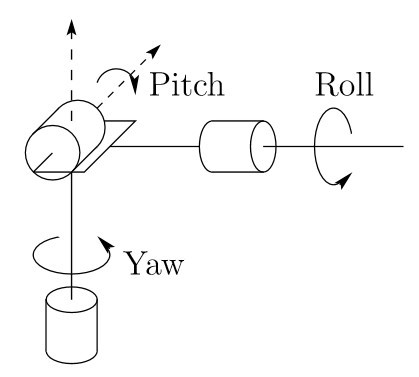
\includegraphics[width=5cm]{gambar/wirst.jpg}
	\caption{Struktur dari \textit{Joint Spherical Wrist}\cite{Spong2006}}
	\label{pic.sphericalwirst}
\end{figure}


\textit{End-effector} merupakan perangkat atau alat yang terhubung dengan ujung lengan robot. \textit{End-effector} adalah bagian robot yang berhubungan langsung dengan objek. Struktur, pergerakan, material dari \textit{end-effector} bergantung pada tugas yang akan dilakukan robot tersebut. Bentuk dari \textit{end-effector} ditunjukkan pada Gambar \ref{pic.endeffector}.
\begin{figure}[H]
	\centering
	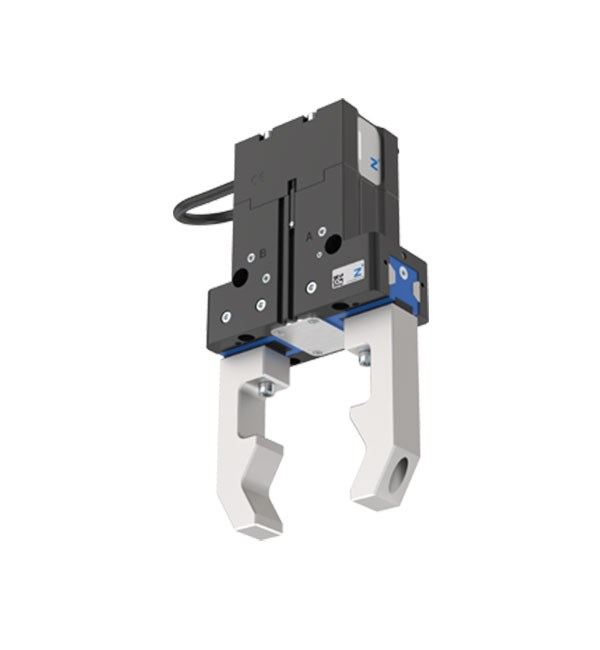
\includegraphics[width=6cm]{gambar/end_effector.jpg}
	\caption{Struktur \textit{End-Effector}\cite{Spong2006}}
	\label{pic.endeffector}
\end{figure}


\section{Kinematika}
Kinematika merupakan pembelajaran pergerakan tubuh robot tanpa memperhitungkan gaya, torsi maupun momen tertentu yang menyebabkan pergerakan. Terdapat berbagai jenis pergerakan dari kinematika tergantung dari tujuan dari setiap robot. Kinematika yang dijelaskan pada penelitian ini adalah kinematika yang khusus mempelajari dan menganalisa pergerakan robot lengan.  

Pada kinematika robot terdapat dua buah pembahasan kinematika. Pembahasan pertama adalah kinematika maju yang merupakan proses menghitung orientasi dan posisi dari\textit{ end-effector} berdasarkan nilai sudut pada masing-masing \textit{joint}.  Sedangkan kinematika balik sebaliknya dari kinematika maju, diberikan posisi \textit{end-effector} dimana akan dicari besaran sudut yang harus diubah untuk tiap \textit{joint} dalam mencapai posisi \textit{end-effector} tersebut\cite{beni}. Diagram blok dari pemodelan kinematika ditunjukkan pada Gambar \ref{pic.diagram.kinematika}. 
\begin{figure}[H]
	\centering
	\includegraphics[width=12cm]{gambar/kinematika_diagram.png}
	\caption{Blok Diagram Kinematika}
	\label{pic.diagram.kinematika}
\end{figure}

\subsection{Kinematika Maju}
Kinematika maju atau biasa disebut \textit{forward kinematics} merupakan kinematika untuk mendapatkan hasil akhir berupa koordinat posisi ($x, y, z$) dengan diketahuinya variabel sudut pada setiap \textit{joint} dari lengan robot.  Variabel sudut tersebut kemudian dilakukan perhitungan satu sama lain hingga pada akhirnya akan mendapatkan koordinat $x$, koordinat $y$, dan koordinat $z$\cite{alasar}. Proses dari kinematika maju ditunjukkan pada Gambar \ref{pic.kinematikamaju}. 
\begin{figure}[H]
	\centering
	
\includegraphics[width=12cm]{gambar/Kinematika_maju.png}
	\caption{Kinematika Maju}
	\label{pic.kinematikamaju}
\end{figure}


\subsection{Kinematika Balik}
Kinematika balik atau biasa disebut \textit{invers kinematics} digunakan untuk mencari variabel sudut (\textit{joint}) robot dalam menentukan posisi dan orientasi dari \textit{end-effector}. Dalam menentukan koordinat \textit{end-effector}, kinematika balik mengacu pada penggunaan persamaan kinematika robot untuk menentukan parameter bersama yang memberikan posisi yang diinginkan pada posisi akhir atau \textit{end-effector}.  Dalam pergerakannya, robot dimodelkan dalam bentuk persamaan kinematika. Persamaan ini menentukan konfigurasi robot dalam hal parameter untuk setiap aktuator. Kinematika maju menggunakan parameter untuk menghitung konfigurasi robot, dan kinematika balik membalikkan perhitungan ini untuk menentukan parameter bersama dalam mencapai konfigurasi yang diinginkan\cite{cahyono2015}. 

Secara garis besar metode kinematika balik mencari nilai parameter yang harus diberikan kepada setiap aktuator untuk mencapai tujuan akhir. Untuk mendapatkan nilai parameter tersebut, robot harus mengetahui terlebih dahulu manipulator yang dimilikinya, baik ukuran maupun jumlah aktuator serta derajat kebebasan yang ada. Kemudian robot harus ditanamkan rumus-rumus yang didapat dari berbagai model perhitungan, baik dari segi analisa grafik langsung maupun menggunakan metode-metode dari berbagai penelitian\cite{cahyono2}. Proses dari kinematika balik ditunjukkan pada Gambar \ref{pic.kinematikabalik}.

\begin{figure}[H]
	\centering
	\includegraphics[width=10cm]{gambar/kinematika_balik.png}
	\caption{Kinematika Balik}
	\label{pic.kinematikabalik}
\end{figure}

\section{Motor DC}
Motor DC adalah motor listrik yang memerlukan tegangan arus searah pada kumparan medan untuk diubah menjadi energi gerak mekanik. Motor DC mempunyai dua bagian utama, yaitu stator dan rotor. Stator merupakan bagian yang tidak berputar dan rotor merupakan bagian yang berputar dan merupakan kumparan jangkar. Motor DC menghasilkan jumlah putaran dalam setiap satuan waktu yang dihitung setiap satuan menit (\textit{rotations per minute}(RPM)) dan arah putaranya dapat diatur searah jarum jam (\textit{clock wise}(CW)) atau berkebalikan dengan arah jarum jam (\textit{counter clock wise}(CCW)) tergantung dengan kutub atau polaritas dari catu daya yang diberikan pada motor DC \cite{dickson}. Bentuk fisik dari motor DC ditunjukkan pada Gambar \ref{pic.motordc}.
\begin{figure}[H]
	\centering
	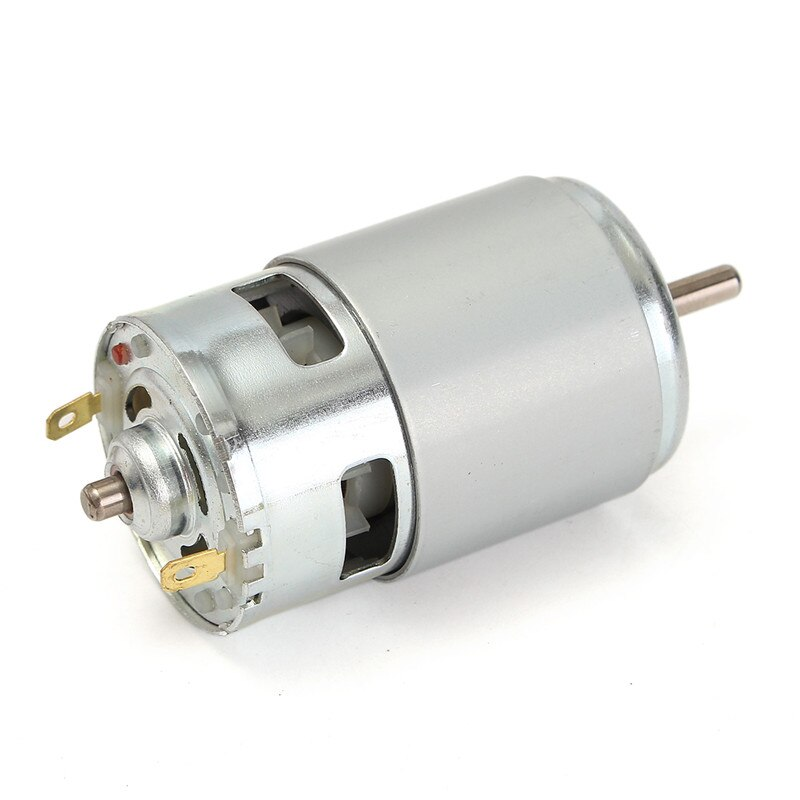
\includegraphics[width=4cm]{gambar/motorDC.jpeg}
	\caption{Bentuk Fisik Motor DC}
	\label{pic.motordc}
\end{figure}

Motor DC dapat bergerak karena adanya elektromagnet. Saat kumparan diberi arus listrik, permukaan kumparan yang bersifat utara akan bergerak menghadap ke magnet yang berkutub selatan dan kumparan yang bersifat selatan akan bergerak menghadap ke utara magnet. Pada saat ini kerena kedua kutub saling menyebabkan pergerakan kumparan berhenti. Untuk menggerakannya lagi tepat pada saat kutub kumparan berhadapan dengan kutub magnet, arah arus pada kumparan dibalik. Dengan demikian, kutub utara kumparan akan berubah menjadi kutub selatan dan kutub selatannya akan berubah menjadi kutub utara\cite{otomotif}.  

Pada saat perubahan kutub tersebut terjadi, kutub selatan kumparan akan berhadapan dengan kutub selatan magnet dan kutub utara kumparan akan berhadapan dengan kutub utara magnet. Karena kutubnya sama, maka akan terjadi tolak menolak sehingga kumparan bergerak memutar hingga utara kumparan berhadapan dengan selatan magnet dan selatan kumparan berhadapan dengan utara magnet. Siklus ini akan berulang-ulang hingga arus listrik pada kumparan diputuskan. Prinsip kerja dari motor DC ditunjukkan pada Gambar \ref{pic.motordcprinsipkerja}.
\begin{figure}[H]
	\centering
	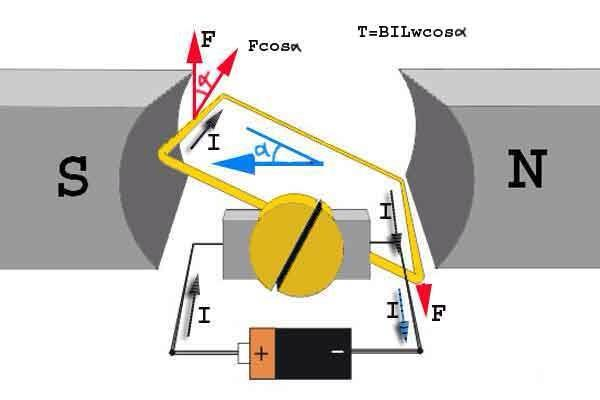
\includegraphics[width=8cm]{gambar/prinsipDC.jpg}
	\caption{Prinsip Kerja Motor DC}
	\label{pic.motordcprinsipkerja}
\end{figure}


\section{Regulator}
Dalam suatu rangkaian elektronika dibutuhkan suatu sumber tegangan yang stabil dan sesuai dengan nilai yang dibutuhkan oleh komponen. Untuk memenuhi kebutuhan tersebut digunakan sebuah rangkaian regulator. Rangkaian regulator berfungsi untuk mengatur atau menghasilkan nilai tegangan pada nilai tertentu dari suatu tegangan masukan. Regulator tegangan mempunyai banyak jenis, salah satunya adalah regulator \textit{switching}\cite{sitohang2018}.

Regulator \textit{switching} mengatur besarnya nilai tegangan keluaran dengan metode mensaklar (ON/OFF) tegangan masukan dengan frekuensi berbeda – beda. Kelebihan dari regulator \textit{switching} adalah adanya disipasi daya yang terjadi lebih kecil dibandingkan dengan regulator linear. Sedangkan kekurangannya yaitu tegangan keluaran akan berbentuk gelombang akibat adanya proses \textit{switching}. Oleh karena itu, regulator jenis ini umumnya membutuhkan induktor, kapasitor, dan dioda untuk menstabilkan tegangan keluaran. Regulator \textit{switching} ada dua jenis yaitu regulator \textit{buck} dan regulator \textit{boost}. Regulator \textit{buck} untuk menghasilkan nilai tegangan keluaran yang lebih kecil dari tegangan masukannya. Sedangkan Regulator \textit{boost} untuk menghasilkan nilai tegangan yang lebih besar dari tegangan masukannya. Salah satu jenis dari regulator \textit{buck} adalah LM2596\cite{semiconductor2008}. Bentuk fisik dari regulator \textit{buck} LM2596 ditunjukkan pada Gambar \ref{pic.lm2596}.

\begin{figure}[H]
	\centering
	\includegraphics[width=7cm]{gambar/lm2596.jpg}
	\caption{Regulator \textit{Buck} LM2596\cite{Minikits}}
	\label{pic.lm2596}
\end{figure}

\section{Arduino Mega 2560}
Arduino Mega 2560  merupakan papan pengembangan dari mikrokontroler yang menggunakan Atmel ATMega2560. Arduino  memiliki pin \textit{input} dan \textit{output} dengan jumlah yang cukup banyak, yaitu sejumlah 54 buah pin \textit{input} dan \textit{output} yang 15 diantaranya merupakan pin \textit{pulse with modulation} (PWM), 16 diantaranya merupakan pin \textit{analog input}, dan terdapat empat pin yang digunakan sebagai \textit{universal asynchronous receiver transmitter} (UART). Arduino ini sudah dilengkapi dengan \textit{oscillator} sebesar 16Mhz, sebuah \textit{port} USB, \textit{power jack} DC, ICSP \textit{header} serta tombol reset \cite{arduino}. Bentuk fisik dari Arduino Mega 2560 ditunjukkan pada Gambar \ref{pic.arudinomega}.
\begin{figure}[H]
	\centering
	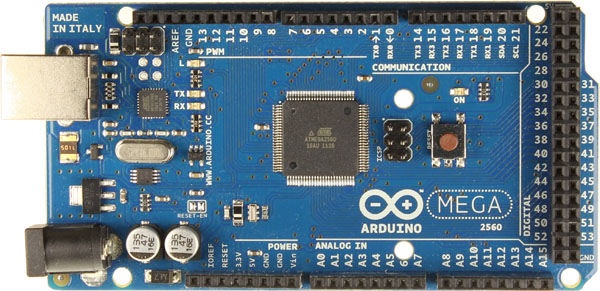
\includegraphics[width=5cm]{gambar/arduino_mega.jpg}
	\caption{Arduino Mega 2560\cite{arduino}}
	\label{pic.arudinomega}
\end{figure}

Arduino Mega 2560 memuat semua yang dibutuhkan untuk mendukung kerja dari sebuah mikrokontroler. Arduino Mega 2560 dapat dengan mudah dioperasikan untuk pengaplikasian ke sebuah sistem kerja karena dapat dihubungkan dengan kabel USB sebagai komunikasinya. Arduino Mega 2560 dapat dihidupkan melalui konektor DC yang dipunyainya dengan diberi tegangan DC, atau baterai dengan nilai tegangan sesuai dengan spesifikasi pada Arduino Mega seperti yang ditunjukkan pada Tabel \ref{tbl.arduinomega}\cite{arduino2}.
\begin{table}[H]
	\centering
	\caption{ Spesifikasi Arduino Mega 2560 }
	\label{tbl.arduinomega}
	\begin{tabular}{|l|l|}
		\hline
		\rowcolor[HTML]{9B9B9B} 
		\multicolumn{1}{|c|}{\cellcolor[HTML]{9B9B9B}Keterangan} & \multicolumn{1}{c|}{\cellcolor[HTML]{9B9B9B}Nilai} \\ \hline
		Mikrokontroler                                           & Atmega2560                                         \\ \hline
		Tegangan Operasional                                     & 5 Volt                                             \\ \hline
		Tegangan Masukan                                         & 5-12 Volt                                          \\ \hline
		Pin Digital I/O                                          & 54 Buah                                            \\ \hline
		Pin PWM                                                  & 15 Buah                                            \\ \hline
		Arus I/O                                                 & 20 mA                                              \\ \hline
		Memori \textit{Flash}                                             & 256 KB                                             \\ \hline
		Kecepatan \textit{Clock}                                          & 16 Mhz                                             \\ \hline
		Dimensi                                                  & 101.52 x 53.3 mm                                   \\ \hline
	\end{tabular}
\end{table}
\section{\textit{Driver} Motor H-\textit{Bridge} EMS 30A}
\textit{Driver} motor H-\textit{Bridge} EMS 30A berfungsi sebagai pengontrol dari setiap pergerakan dari arah putar dan kecepatan pada motor DC. Umunya \textit{driver} motor memiliki beberapa jenis tergantung dari spesifikasi dari motor DC yang digunakan. Salah satu jenis \textit{driver} motor adalah \textit{driver} Motor  H-\textit{Bridge} EMS 30A. Bentuk fisik dari \textit{driver} Motor H-\textit{Bridge} EMS 30A ditunjukkan pada Gambar \ref{pic.drivermotor}.
\begin{figure}[H]
	\centering
	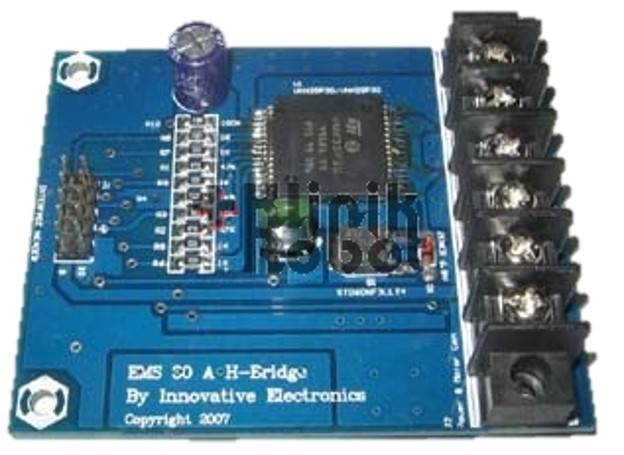
\includegraphics[width=5cm]{gambar/driver_motor.jpg}
	\caption{\textit{Driver} Motor EMS 30A H-\textit{Bridge}}
	\label{pic.drivermotor}
\end{figure}

Driver ini memiliki 10 buah pin data yang dapat dihubungkan dengan sebuah mikrokontroler. Tabel \ref{tbl.pindrivermotor} merupakan alokasi pin pada \textit{driver} motor H-\textit{Bridge} EMS 30A.

% Please add the following required packages to your document preamble:
% \usepackage[table,xcdraw]{xcolor}
% If you use beamer only pass "xcolor=table" option, i.e. \documentclass[xcolor=table]{beamer}
% \usepackage[normalem]{ulem}
% \useunder{\uline}{\ul}{}
\begin{table}[H]
	\centering
	\caption{ Pin pada \textit{Driver} EMS 30A H-\textit{Bridge} }
	\label{tbl.pindrivermotor}
	\begin{tabular}{|c|c|c|l|}
		\hline
		\rowcolor[HTML]{9B9B9B} 
		Pin  & Nama & I/O & \multicolumn{1}{c|}{\cellcolor[HTML]{9B9B9B}Fungsi}                                                                                                                         \\ \hline
		1    & MIN1 & I   & Pin \textit{input} untuk menentukan \textit{output} MOUT1                                                                                                                                     \\ \hline
		2    & MIN2 & I   & Pin \textit{input} untuk menentukan \textit{output} MOUT2                                                                                                                                     \\ \hline
		3    & MEN1 & I/O & \begin{tabular}[c]{@{}l@{}}Pin \textit{enable} untuk \textit{output} MOUT1 \\ diberi logika HIGH untuk mengaktifkan \textit{half} H-\textit{Bridge} 1, \\ diberi logika LOW untuk menonaktifkannya\end{tabular} \\ \hline
		4    & MEN2 & I/O & \begin{tabular}[c]{@{}l@{}}Pin \textit{enable} untuk \textit{output} MOUT2 \\ diberi logika HIGH untuk mengaktifkan \textit{half} H-\textit{Bridge} 2, \\ diberi logika LOW untuk menonaktifkannya\end{tabular} \\ \hline
		5    & MSC  & O   & \textit{Output} tegangan analog yang berbanding lurus dengan arus beban                                                                                                              \\ \hline
		6    & MPWM & I   & Pin \textit{input} untuk mengatur kerja modul H-\textit{Bridge} secara PWM                                                                                                                    \\ \hline
		7,9  & VCC  & -   & Terhubung ke catu daya untuk \textit{input} (5 Volt)                                                                                                                                 \\ \hline
		8,10 & PGND & 0   & Titik referensi untuk catu daya \textit{input}                                                                                                                                       \\ \hline
	\end{tabular}
\end{table}
\section{Processing \textit{Integrated Development Environment} (IDE)}
Processing IDE adalah pemrograman yang diciptakan untuk pengembangan aplikasi yang berorientasi visual atau pencitraan dengan penekanan pada animasi dan memberi pengguna umpan balik melalui interaksi antarmuka. Para \textit{developer} Processing IDE ini menginginkan sebuah cara untuk "membuat sketsa" gagasan dalam bentuk kode. Karena pemrograman telah berkembang selama beberapa dekade terakhir. Processing IDE telah mulai digunakan untuk pekerjaan tingkat produksi yang lebih maju. Awalnya dibangun sebagai ekstensi khusus \textit{domain} Java yang ditargetkan untuk seniman dan desainer, Processing IDE telah berkembang menjadi alat desain dan prototipe lengkap dan penuh yang digunakan untuk pekerjaan instalasi skala besar, grafis gerak, dan visualisasi data yang rumit\cite{aku2012}. Tampilan pada Processing IDE ditunjukkan pada Gambar \ref{pic.processingide}.
\begin{figure}[H]
	\centering
	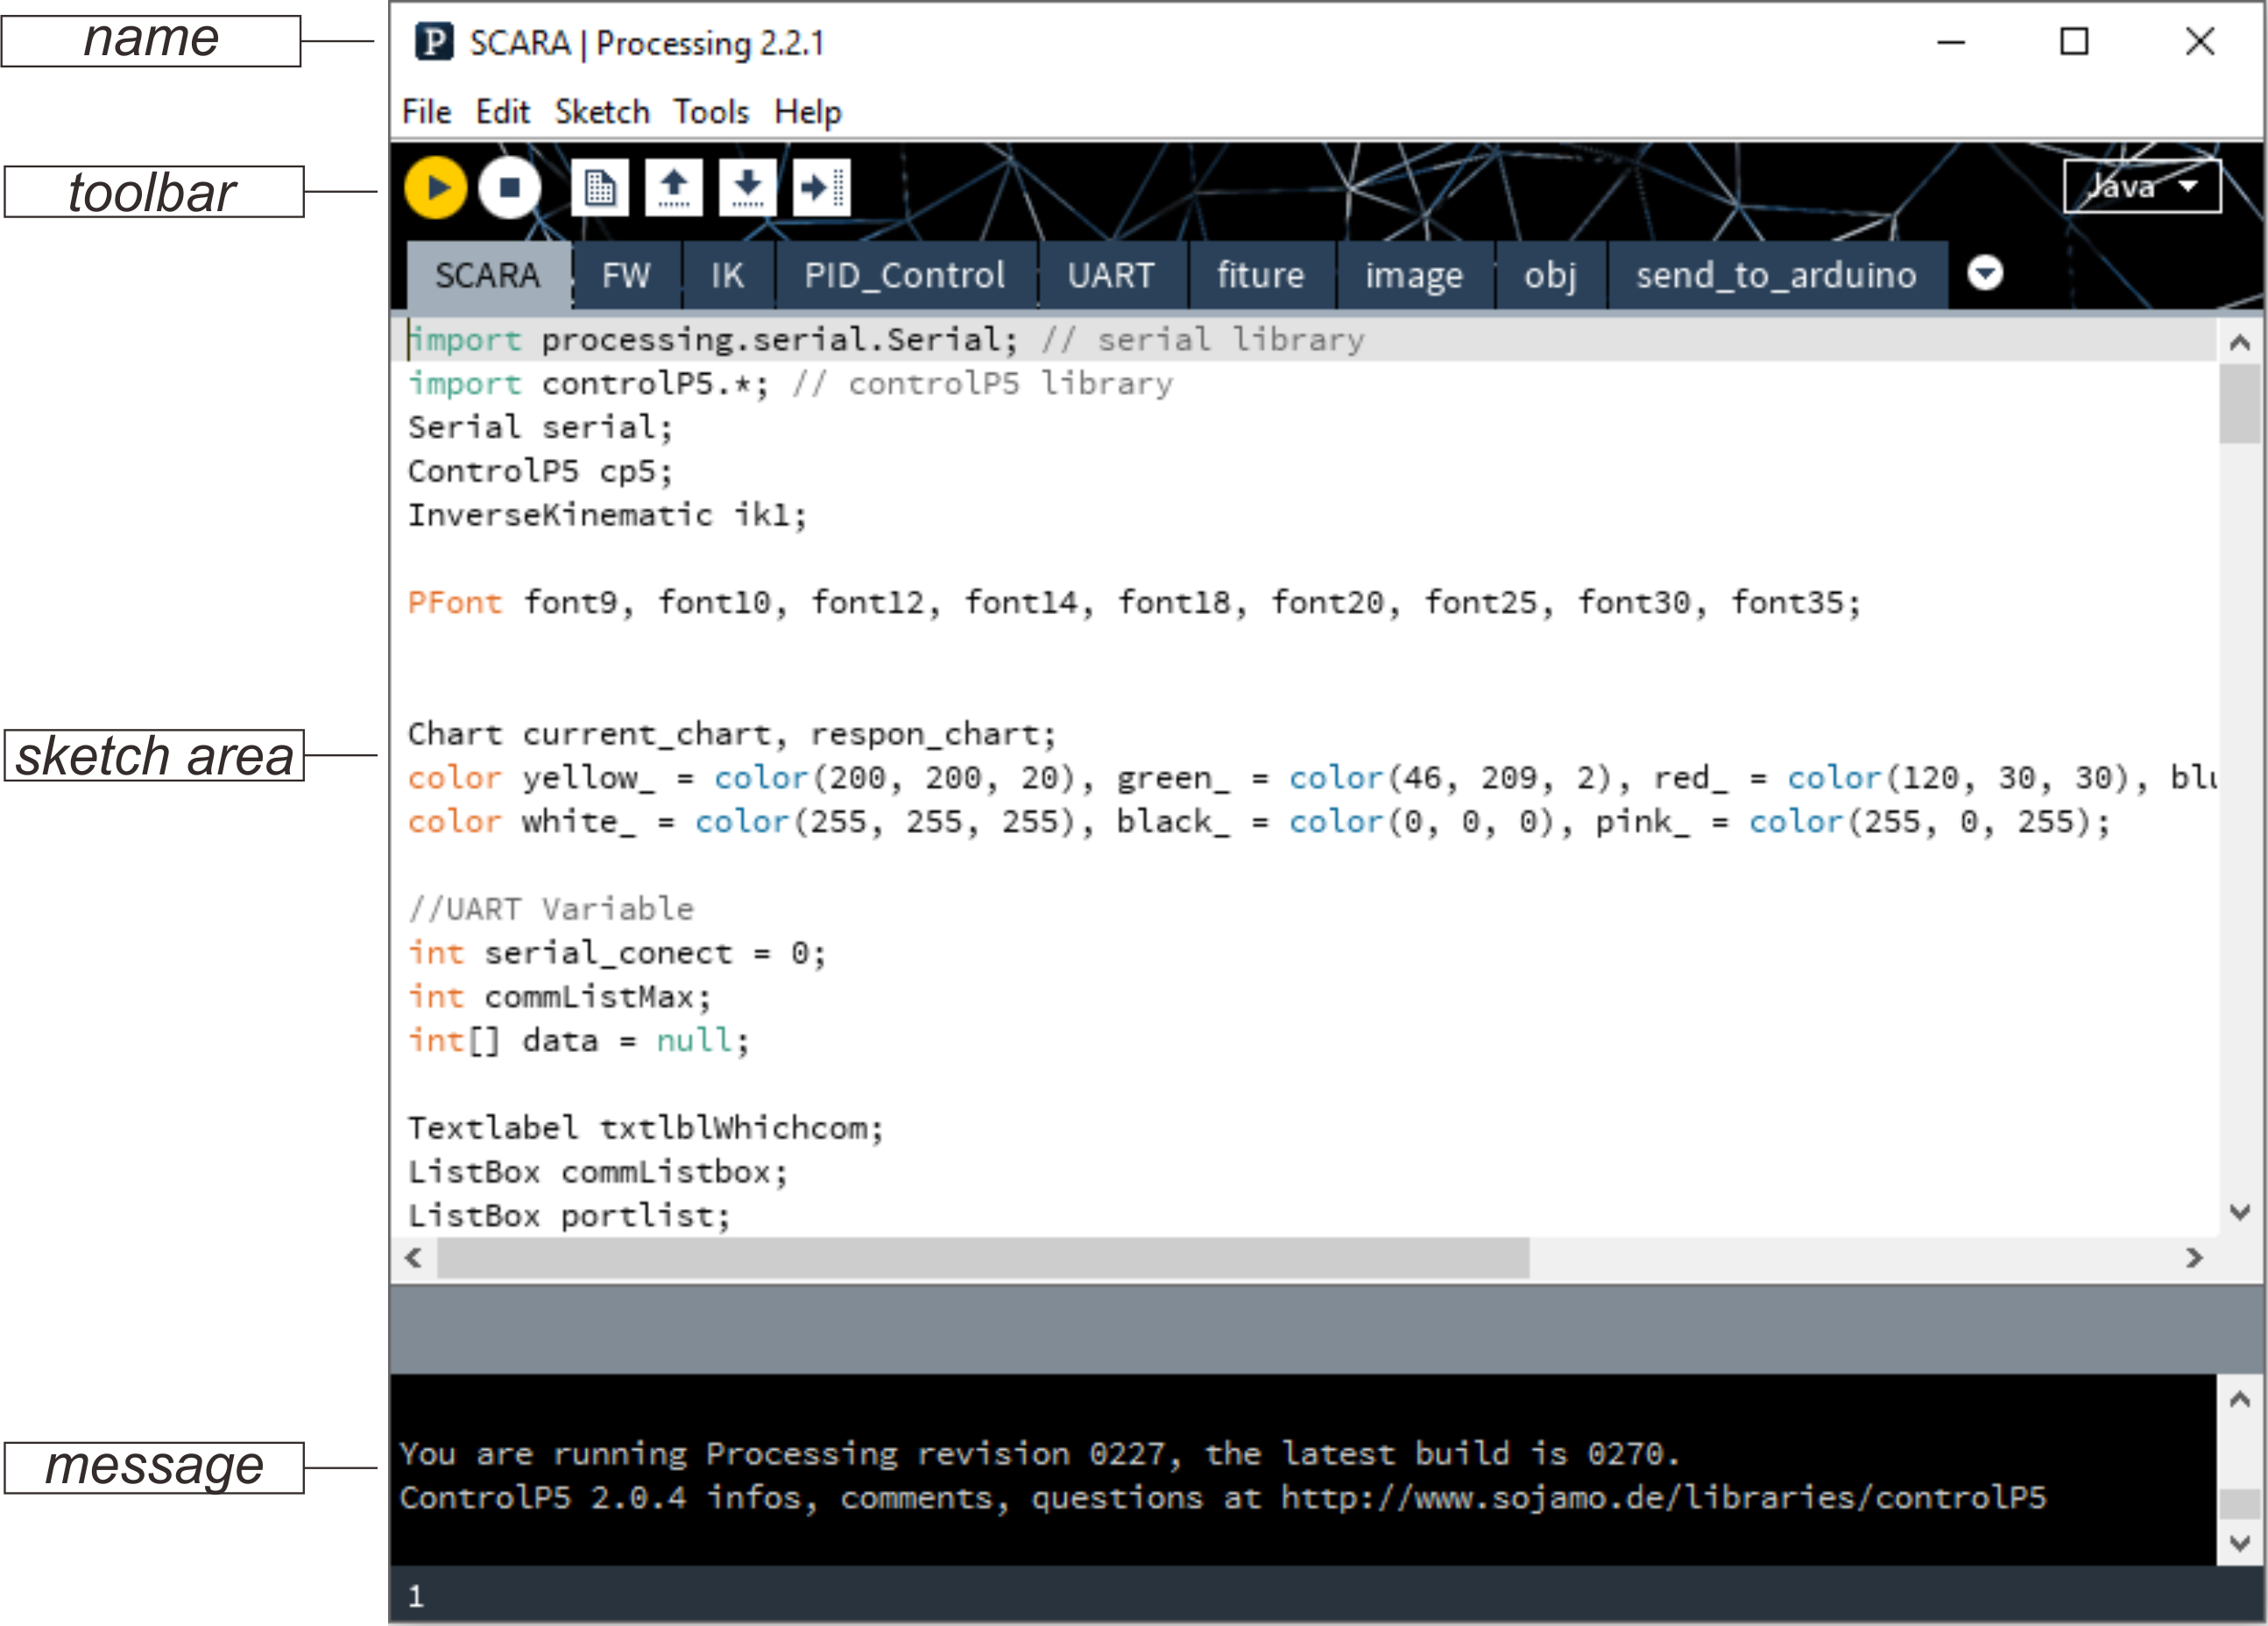
\includegraphics[width=12cm]{gambar/processing_view.png}
	\caption{Tampilan Processing IDE}
	\label{pic.processingide}
\end{figure}


\subsection{\textit{Syntax} dalam Processing IDE }

\subsubsection{Mengatur Ukuran}
Ukuran sebuah objek pada Processing IDE diatur menggunakan sebuah \textit{syntax} size(). Fungsi size() digunakan untuk menetapkan variabel global lebar dan tinggi dari suatu program. Ukuran untuk panjang dan tinggi tersebut menggunakan ukuran piksel. Lebar diwakili dengan variabel "\textit{width}" dan tinggi diwakili dengan variabel "\textit{height}". Untuk objek yang ukurannya tergantung pada layar, selalu gunakan variabel lebar dan tinggi, bukan angka. Ini mencegah masalah saat parameter fungsi size() diubah.


\subsubsection{Transformasi Bentuk dalam Processing IDE }
Transformasi pada Processing IDE digunakan untuk memindahkan, memutar atau, mengecilkan atau membesarkan suatu objek dan perpindahannya dapat diatur dengan parameter-parameter tertentu di dalam Processing IDE. Transformasi adalah dasar dari pemrograman Processing IDE. Contoh penulisan \textit{syntax} dari transformasi ditunjukkan pada Tabel \ref{tbl.syntxtransformasi}.

% Please add the following required packages to your document preamble:
% \usepackage[table,xcdraw]{xcolor}
% If you use beamer only pass "xcolor=table" option, i.e. \documentclass[xcolor=table]{beamer}
\begin{table}[H]
	\centering
	\caption{ \textit{Syntax} Transformasi}
	\label{tbl.syntxtransformasi}
	\begin{tabular}{|c|l|l|}
		\hline
		\rowcolor[HTML]{9B9B9B} 
		No & \multicolumn{1}{c|}{\cellcolor[HTML]{9B9B9B}Syntax} & \multicolumn{1}{c|}{\cellcolor[HTML]{9B9B9B}Keterangan}                                    \\ \hline
		1  & Translate(x,y)                                      & \begin{tabular}[c]{@{}l@{}}x = transisi kiri/kanan \\ y = transisi atas/bawah\end{tabular} \\ \hline
		2  & Rotate(\textit{angle})                                       & \textit{angle}=besar sudut rotasi(radian)                                                           \\ \hline
		3  & RotateX(\textit{angle})                                      & \textit{angle}=besar sudut rotasi(radian)                                                           \\ \hline
		4  & RotateY(\textit{angle})                                      & \textit{angle}=besar sudut rotasi(radian)                                                           \\ \hline
		5  & Rotatez(\textit{angle})                                      & \textit{angle}=besar sudut rotasi(radian)                                                           \\ \hline
		6  & Scale(S)                                            & s = besar pengecilan pembesaran                                                            \\ \hline
	\end{tabular}
\end{table}
\subsubsection{\textit{Shape}}
\textit{Shape} adalah \textit{syntax} pada Processing IDE yang berfungsi untuk membuat berbagai macam bentuk, seperti persegi panjang, lingkaran, garis, dan bentuk lainnya yang dapat diatur ukurannya dengan parameter-parameter tertentu. Tabel \ref{tbl.syntxshape} merupakan contoh dari beberapa \textit{syntax} shape. 
\begin{table}[H]
	\centering
	\caption{\textit{Syntax} Shape}
	\label{tbl.syntxshape}
	\resizebox{14cm}{!}{%
		\begin{tabular}{|l|l|l|l|}
			\hline
			\rowcolor[HTML]{9B9B9B} 
			
			No & Sytax                          & Bentuk & Keterangan                                                                                                                                                                                    \\ \hline
			1  & ellipse(a,b,c,d)               &  	\centering 
\includegraphics[width=3cm]{gambar/bulat.png} 
			& \begin{tabular}[c]{@{}l@{}}a = koordinatX \\ b = koordinatY \\ c= lebar diameter \\ d= tinggi diameter\end{tabular}                                                                           \\ \hline
			2  & arc(a,b,c,d,start,st op,moode) &  	
\includegraphics[width=3cm]{gambar/busur.png}    \centering  & \begin{tabular}[c]{@{}l@{}}a = koordinatX \\ b = koordinatY \\ c = lebar diameter \\ d = tinggi diameter \\ start = sudut mulai \\ stop = sudut akhir \\ mode = PIE, CHORD, OPEN\end{tabular} \\ \hline
			3  & line(x1,y1,x2,y2)              & 	
\includegraphics[width=3cm]{gambar/garis.png}       & \begin{tabular}[c]{@{}l@{}}x1 = koordinatX1 \\ y1 = koordinatY1 \\ x2 = koordinatX2 \\ y2 = koordinatY2\end{tabular}                                                                          \\ \hline
			4  & point(x,y)                     &     	
\includegraphics[width=3cm]{gambar/point.png}   & \begin{tabular}[c]{@{}l@{}}x = koordinatX \\ y = koordinatY\end{tabular}                                                                                                                      \\ \hline
			5  & rect(a,b,c,d,r)                &    	
\includegraphics[width=3cm]{gambar/kotak.png}    & \begin{tabular}[c]{@{}l@{}}a = koordinatX1 \\ b = koordinatY1 \\ c = koordinatX2 \\ d= koordinatY1\end{tabular}                                                                               \\ \hline
	\end{tabular}}
\end{table}

\subsubsection{Akses Koordinat \textit{Mouse} }
Processing IDE mempunyai fungsi khusus yaitu dapat melacak posisi \textit{mouse} baik secara vertical maupun horizontal. Namun, Processing IDE hanya dapat melacak posisi \textit{mouse} saat \textit{sketch} dijalankan saja. Nilai \textit{default} mouseX dan mouseY adalah 0, jadi 0 akan dikembalikan sampai \textit{mouse} bergerak di depan jendela sketsa. Setelah \textit{mouse} bergerak menjauh dari jendela, mouseX akan terus melaporkan posisi terakhirnya.  Contoh penulisan \textit{syntax} dari \textit{mouse} ditunjukkan pada Tabel \ref{tbl.koordinatmouse}.
\begin{table}[H]
	\centering
	\caption{\textit{Syntax} Koordinat \textit{Mouse}}
	\label{tbl.koordinatmouse}
	\begin{tabular}{|c|l|l|}
		\hline
		\rowcolor[HTML]{9B9B9B} 
		No & \multicolumn{1}{c|}{\textit{Syntax}} & \multicolumn{1}{c|}{Keterangan}                                                                                                 \\ \hline
		1  & mouseX                               & \begin{tabular}[c]{@{}l@{}}Variabel sistem X memiliki nilai dari \\ koordinat horizontal \textit{mouse} secara \textit{real time}\end{tabular}    \\ \hline
		2  & mouseY                               & \begin{tabular}[c]{@{}l@{}}Variabel sistem Y memiliki nilai dari koordinat \\ horizontal \textit{mouse} secara \textit{real time}.\end{tabular}   \\ \hline
		3  & mouseButton()                        & \begin{tabular}[c]{@{}l@{}}Bila tombol \textit{mouse} ditekan, nilai \textit{variable} sistem \\ diatur ke \textit{left}, \textit{right}, atau \textit{center}.\end{tabular} \\ \hline
		4  & mouseClicked()                       & \begin{tabular}[c]{@{}l@{}}Dipanggil setelah tombol \textit{mouse} ditekan dan kemudian dilepaskan.\end{tabular}                      \\ \hline
		5  & mouseDragged()                       & Dipanggil setelah tombol \textit{mouse} bergerak saat ditekan.                                                                           \\ \hline
	\end{tabular}
\end{table}

\subsubsection{ \textit{Compile Sketch} }
Program pada Processing IDE dinamakan \textit{sketch}. Tujuan diberi nama \textit{sketch} adalah untuk membuat pemrograman bergaya Java ini terasa lebih seperti \textit{scripting}, dan mengadopsi proses \textit{scripting} untuk menulis kode dengan cepat. \textit{Sketch} disimpan dalam bentuk \textit{Sketchbook}. Gambar \ref{pic.toolbarsketch} merupakan \textit{toolbar} dari \textit{sketch.}

\begin{figure}[H]
	\centering
	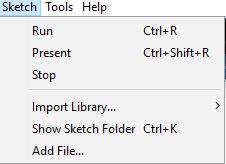
\includegraphics[width=5cm]{gambar/compile.jpg}
	\caption{\textit{Toolbar Sketch}}
	\label{pic.toolbarsketch}
\end{figure}

\subsection{ \textit{Library} untuk Processing IDE }
\subsubsection{ Memuat Huruf (\textit{Pfont}) pada Processing IDE }
Pfont adalah \textit{class} yang digunakan untuk penggunaan \textit{font} pada Processing IDE. Untuk membuat \textit{font} yang akan digunakan dengan Processing IDE, diawali dengan memilih "\textit{Create Font ...}" dari menu \textit{Tools}. Ini akan membuat \textit{font} dalam \textit{format} Processing IDE yang membutuhkan dan juga menambahkannya ke direktori data sketsa saat ini. Pengolahan menampilkan \textit{font} menggunakan format \textit{font} .vlw. Fungsi loadFont() digunakan untuk membuat \textit{font} baru dan textFont () digunakan agar \textit{font} baru yang telah dibuat tersebut aktif. \textit{Syntax} list() berfungsi untuk membuat daftar \textit{font} yang terunduh pada komputer yang merupakan informasi yang berguna untuk digunakan dengan fungsi createFont() untuk mengubah \textit{font} secara dinamis menjadi format yang bisa digunakan di Processing IDE. 


\subsubsection{ Memuat ControlP5 pada Processing IDE }
ControlP5 adalah \textit{library} yang berfungsi sebagai pengontrol untuk membuat antarmuka dengan \textit{user}, ControlP5 berupa grafis di dalam \textit{sketch} Processing IDE yang meliputi \textit{slider}, \textit{button}, \textit{toggles}, \textit{knobs}, \textit{radiobutton}, dan dapat dengan mudah ditambahkan ke \textit{sketch} pengolahan. ControlP5 ditulis oleh Andreas Schlegel untuk pemrograman Processing IDE. \textit{Library} ControlP5 bisa diunduh di laman https://github.com/sojamo/controlp5 atau unduh di \textit{library} Processing IDE secara langsung. Gambar \ref{pic.controlp5} merupakan beberapa contoh gambaran dari ControlP5.
\begin{figure}[H]
	\centering
	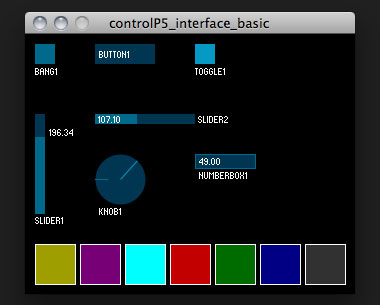
\includegraphics[width=8cm]{gambar/controlp5.jpg}
	\caption{ControlP5}
	\label{pic.controlp5}
\end{figure}
Setiap \textit{tools} yang ada pada ControlP5 memiliki fungsi yang berbeda-beda sesuai dengan kegunaannya. ControlP5 dapat dipakai atau saling dikombinasikan agar memudahkan dan memaksimalkan dari GUI yang telah dibuat. ControlP5 nantinya akan bekerja sesuai dengan program yang sudah dimasukkan. Beberapa fungsi dari \textit{tools} yang ada pada ControlP5 ditunjukkan pada Tabel \ref{tbl.toolscontrolp5}.
% Please add the following required packages to your document preamble:
% \usepackage[table,xcdraw]{xcolor}
% If you use beamer only pass "xcolor=table" option, i.e. \documentclass[xcolor=table]{beamer}
\begin{table}[H]
	\centering
	\label{tbl.toolscontrolp5}
	\caption{ Fungsi dari \textit{tools} ControlP5}
	\begin{tabular}{|c|l|l|}
		\hline
		\rowcolor[HTML]{9B9B9B} 
		No & \multicolumn{1}{c|}{\cellcolor[HTML]{9B9B9B}ControlP5} & \multicolumn{1}{c|}{\cellcolor[HTML]{9B9B9B}Fungsi}                                                                                                                                                 \\ \hline
		\rowcolor[HTML]{FFFFFF} 
		1  & Bang                                                   & \begin{tabular}[c]{@{}l@{}}Memicu sebuah tindakan ketika ditekan\\ controlP5.addBang("bang1");\end{tabular}                                                                                         \\ \hline
		2  & Button                                                 & \begin{tabular}[c]{@{}l@{}}Memicu sebuah tindakan ketika sudah dilepas\\ controlP5.addButton("button1");\end{tabular}                                                                               \\ \hline
		3  & Toggle                                                 & \begin{tabular}[c]{@{}l@{}}\begin{tabular}[c]{@{}l@{}}Memiliki dua status. \\ \textit{true} meiliki nilai 1 dan \textit{false} memiliki nilai 0\end{tabular}\\ controlP5.addToggle("toggle1")\end{tabular}            \\ \hline
		4  & Slider                                                 & \begin{tabular}[c]{@{}l@{}}\begin{tabular}[c]{@{}l@{}}Mengatur nilai dengan cara menggeser \\ secara horisontal maupun vertikal\end{tabular}\\ controlP5.addSlider("slider2");\end{tabular}         \\ \hline
		5  & Knob                                                   & \begin{tabular}[c]{@{}l@{}}Mengatur sebuah nilai dengan tombol putaran 360°\\ controlP5.addKnob("knob1");\end{tabular}                                                                              \\ \hline
		6  & NumberBox                                              & \begin{tabular}[c]{@{}l@{}}\begin{tabular}[c]{@{}l@{}}Kotak yang menampilkan angka dan \\ dapat diubah dengan klik di dalam kotak\end{tabular}\\ controlP5.addNumberbox("numberbox1");\end{tabular} \\ \hline
	\end{tabular}
\end{table}
%BAB_3 LAPORAN KP

\chapter{PERANCANGAN SISTEM}
Pada bab ini akan disajikan mekanisme perancangan alat baik perangkat keras ataupun perangkat lunak untuk mewujudkan sebuah robot lengan. Tahapan perancangan dimulai dari perancangan diagram blok sistem, perancangan perangkat keras, perancangan perangat lunak, perancangan kinematika balik, perancangan GUI, dan integrasi keseluruhan program. 
\section{ Diagram Blok Sistem }
Secara garis besar pada tahapan implementasi dari kinematika pada robot lengan SCARA ini menggunakan \textit{output} atau penggerak berupa motor DC dengan \textit{feedback} posisi berupa \textit{potensiometer} sedangkan pada bagian  \textit{input} yang berasal dari GUI yang dibuat pada Processing IDE mengirimkan sebuah koordinat yang digunakan untuk menentukan pergerakan robot berdasarkan fungsi \textit{inverse kinematic}. Gambar \ref{pic.diagram.bloksistem} merupakan diagram blok sistem secara keseluruhan.
\begin{figure}[H]
	\centering
	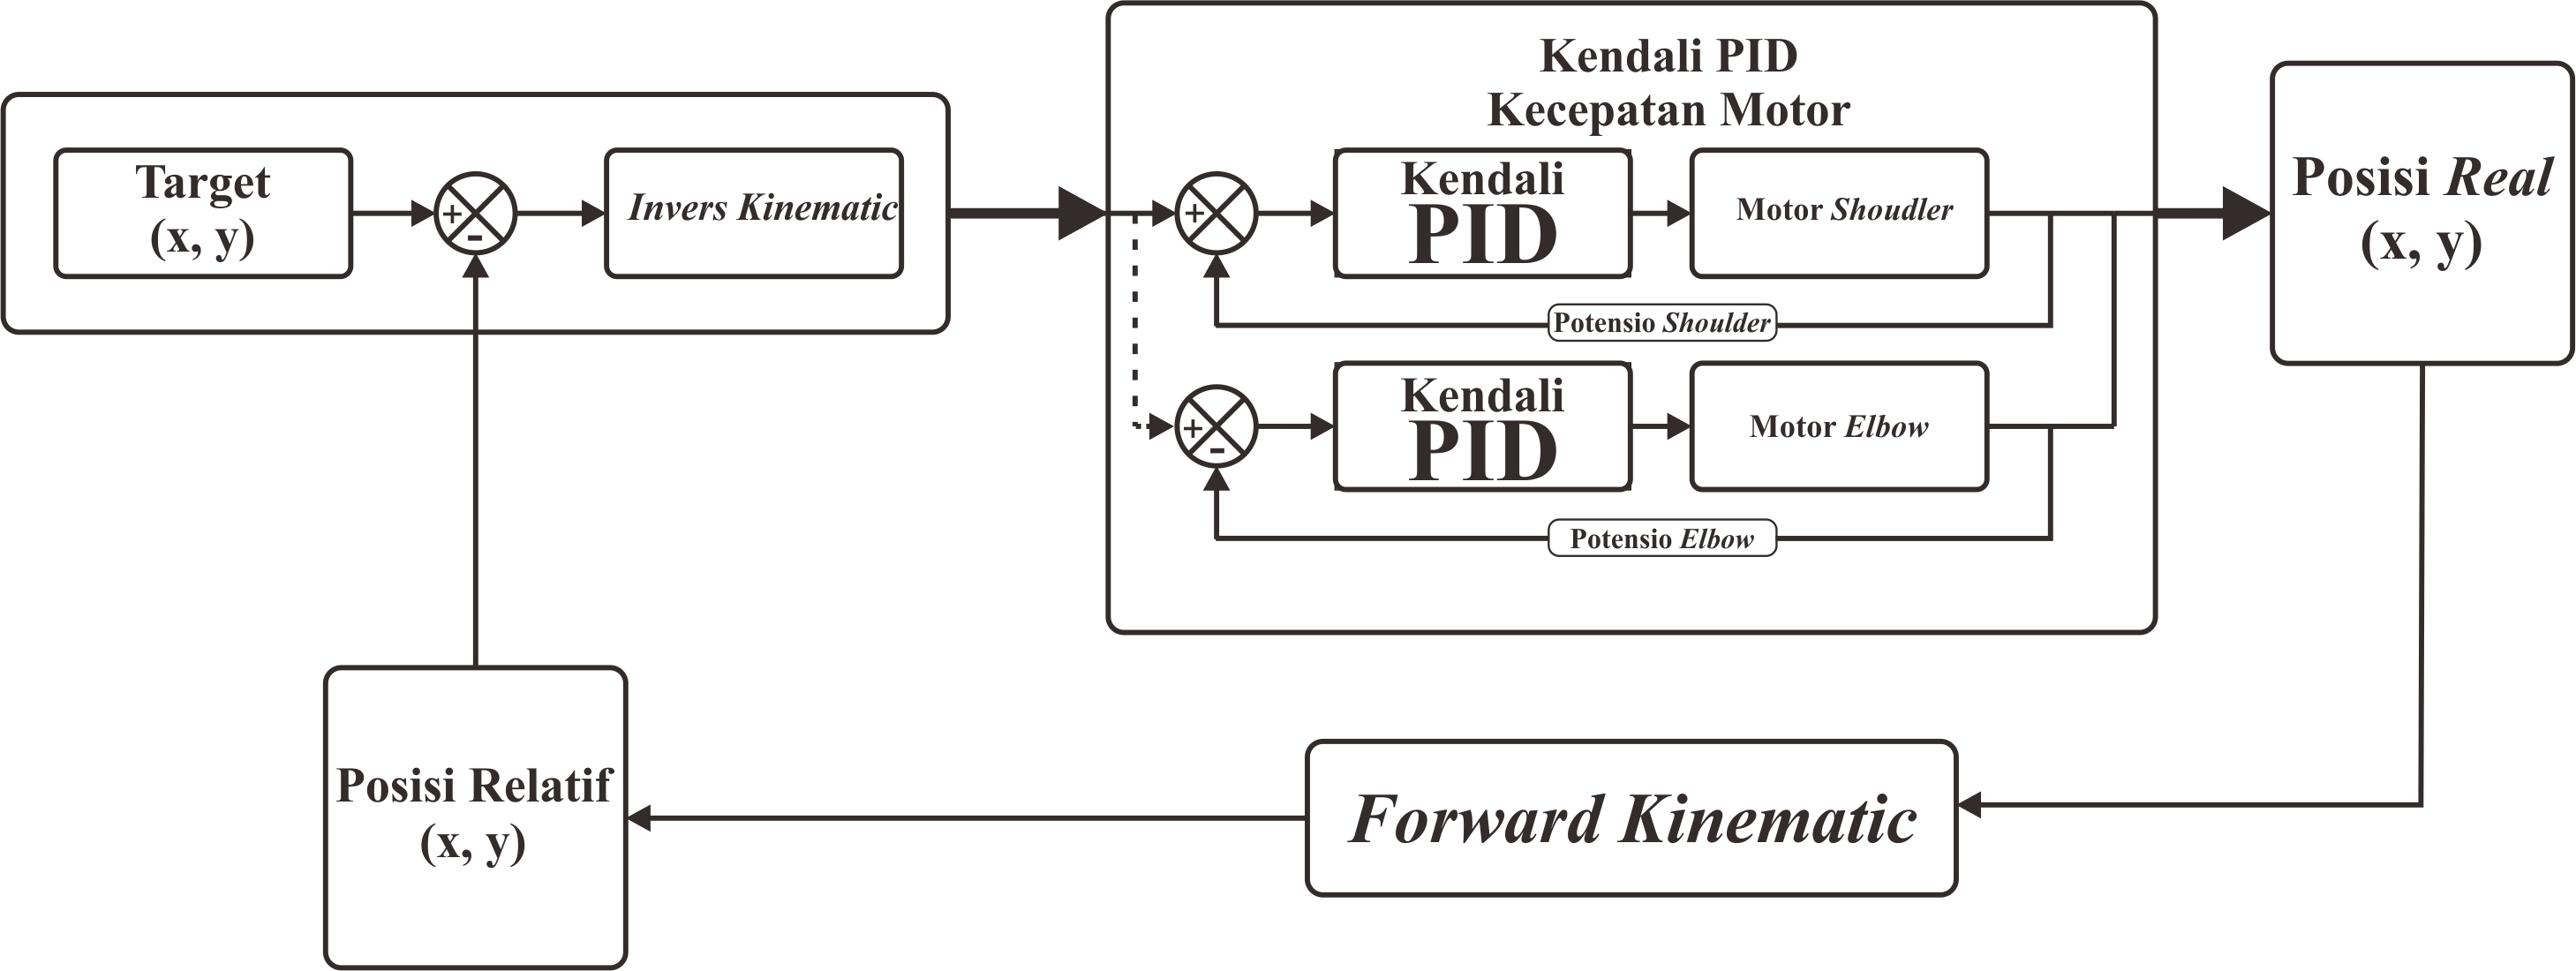
\includegraphics[width=13cm]{gambar/diagram_blok_new.png}
	\caption{Diagram Blok Sistem}
	\label{pic.diagram.bloksistem}
\end{figure}
Pada blok diagram yang disajikan pada Gambar \ref{pic.diagram.bloksistem} sistem terdiri dari bagian – bagian yang meliputi bagian masukan, bagian kendali, bagian keluaran, dan bagian penampil. Pada bagian masukan menggunakan GUI yang dirancang pada Processing IDE yang digunakan sebagai \textit{forward kinematic} serta \textit{inverse kinematic} dimana robot akan bergerak menyesuaikan dengan posisi atau sudut yang dimasukan melauli Processing IDE. 
Pada bagian kontrol menggunakan Arduino Mega 2560 sebagai mikrokontroler yang mengendalikan seluruh operasi dari robot. \textit{Power supply} Arduino sebesar 5 volt DC didapatkan dari regulator tegangan yang menurunkan tegangan dari 24 volt DC ke 5 volt DC. 

Pada bagian keluaran, pin \textit{pulse with modulation} (PWM) pada Arduino Mega 2560 dihubungkan dengan \textit{driver} motor yang digunakan untuk mengontrol arah pergerakan dari motor DC serta kecepatan pergerakan dari motor DC. Pergerakan arah putaran motor DC bergantung pada \textit{feedback} posisi setiap sendi yang diberikan oleh potensiometer. Tiga buah pin digital pada Ardunio Mega 2560 dihubungkan pada rangkaian \textit{switch} yang menggunakan IC TIP31 yang berfungsi sebagai kontrol dari \textit{end-effector} yang dioperasikan menggunakan tekanan udara yang dikontrol oleh \textit{valve pneumatic.}

Pada bagian penampil merupakan bentuk dari rancangan GUI yang dirancang dalam Processing IDE melalui sebuah bentuk pemrograman. Dalam tampilan GUI terdapat beberapa \textit{tools} yang dapat untuk mengatur pergerakan robot SCARA. Pada GUI menampilkan nilai dari sudut, dan posisi serta animasi robot SCARA pada kondisi langsung dari pergerakan robot SCARA.
\section{ Perancangan Perangkat Keras }
Perancangan perangkat keras pada robot lengan SCARA terdiri dari dua bagian yaitu bagian mekanis dan elektronis. Bagian  mekanis merupakan bagian \textit{hardware} yang meliputi desain, bahan dan bentuk dari\textit{ arm manipulator robot} SCARA. Bagian elektronis merupakan bagian \textit{hardware} yang meliputi sistem – sistem yang berkaitan dengan rangkaian pada robot SCARA seperti rangkaian pada desain \textit{board} serta komponen – komponen elektronis pendukung.
\subsection{ Sistem Mekanis }
Sistem memkanis dari robot lengan bergantung dari konfigurasi robot lengan. Konfigurasi robot lengan terbagi menjadi enam, yaitu konfigurasi \textit{articulated}, konfigurasi SCARA, konfigurasi \textit{spherical}, konfigurasi \textit{cylindrical}, dan konfigurasi \textit{cartesian}. Pada peneltian KP, konfigurasi robot lengan yang digunakan adalah konfigurasi SCARA dengan dua \textit{joint} \textit{revolute} dan satu \textit{joint prismatic}. Sistem mekanik dari lengan robot tiga DOF sangat berpengaruh dan mendominasi sistem karena bentuk dan pergerakan dari mekanik akan mempengaruhi elektronis serta program. Sistem mekanik yang baik sangat mendukung dari pergerakan robot, oleh karena itu perancangan mekanik harus proporsional dari panjang setiap lengan, lebar serta tinggi robot. \textit{Free body} dari robot SCARA ditunjukkan pada Gambar \ref{pic.freebodyscara}. Bentuk fisik dari robot SCARA yang digunakan pada penelitian ini ditunjukkan pada Gambar \ref{pic.fisikscara}. 
\begin{figure}[H]
	\centering
	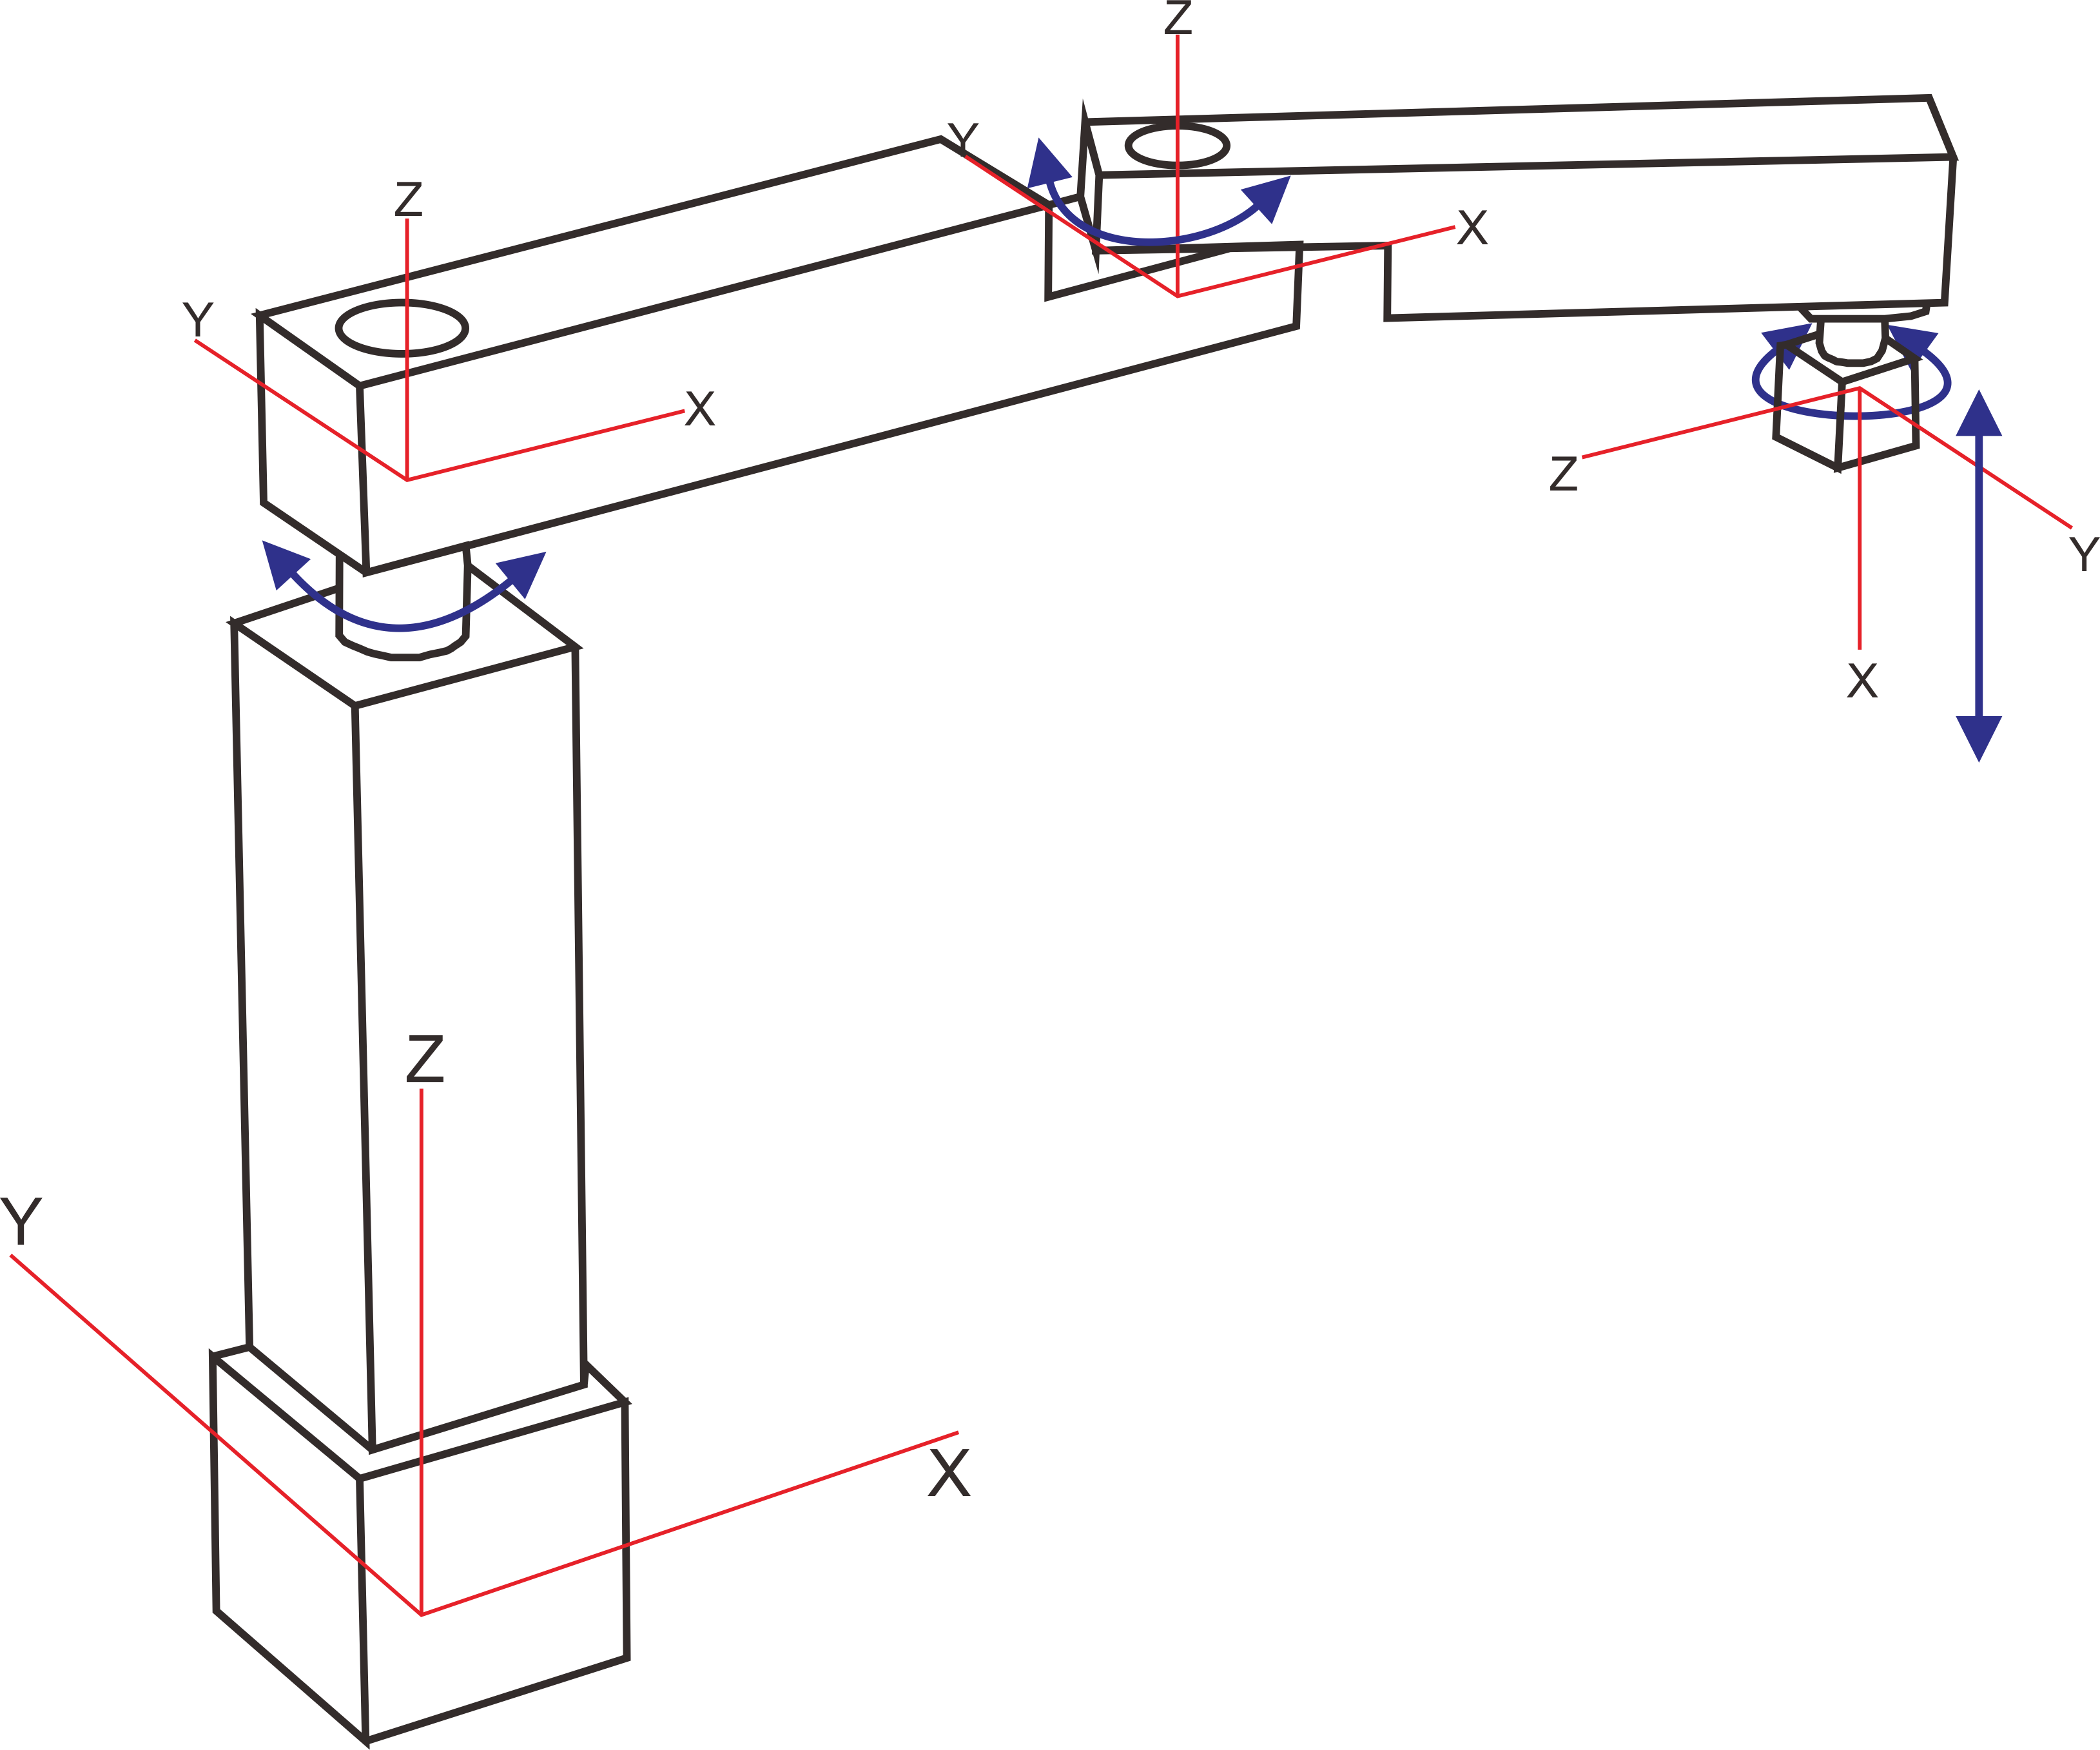
\includegraphics[width=7cm]{gambar/scaraa.png}
	\caption{\textit{Free Body} Robot SCARA}
	\label{pic.freebodyscara}
\end{figure}
\begin{figure}[H]
	\centering
	\includegraphics[width=7cm]{gambar/3dscara.png}
	\caption{Bentuk Fisik Robot SCARA}
	\label{pic.fisikscara}
\end{figure}
Robot SCARA merupakan robot yang meiliki tiga buah derajat kebebasan (DOF) yang terletak pada \textit{shoulder}, \textit{elbow}, dan \textit{end-effector}. Seluruh derajat kebebasan menggunakan sebuah motor DC yang didalamnya terdapat\textit{ gear box}. Motor DC pada \textit{end-effector} dibantu oleh sebuah \textit{belt} untuk menyalurkan putaran dari motor yang terletak pada atas \textit{shoulder}. Pergerakan pada masing-masing \textit{joint} memiliki jangkauan maksimum yang berbeda-beda. Jangkauan dipengaruhi oleh panjangnya lengan yang dimiliki oleh robot SCARA tersebut\cite{bulet}. Spesifikasi dari robot SCARA yang digunakan paad penelitian ini ditunjukkan pada Tabel \ref{tbl.spesifikasiscara}. 

\begin{longtable}{|c|l|}
	\caption{Sistem Elektronis SCARA}
	\label{tbl.elektronisscara}\\
	\hline
	\rowcolor[HTML]{9B9B9B} 
	Keterangan & \multicolumn{1}{c|}{\cellcolor[HTML]{9B9B9B}Nilai} \\ \hline
	\endfirsthead
	%
	\endhead
	%
	 Panjang lengan utama & 360 mm                                             \\ \hline
	Panjgan lengan depan  & 290 mm                                                    \\ \hline
	Gerakan \textit{shoulder}  &180 °                                  \\ \hline
	Gerakan \textit{elbow}  & 200 °                                  \\ \hline
	Rotasi \textit{end-effector}  & 360 °                                   \\ \hline
	Pergerakan naik dan turun \textit{end-effector}  &  150 mm                            \\ \hline
	Berat objek maksimum  &  3.0 kg                                                 \\ \hline

\end{longtable}

Desain pada\textit{ arm manipulator robot} SCARA berbahan besi dengan tebal 2 mm dengan tiga derajat kebebasan yang meliputi bagian \textit{shoulder}, \textit{elbow} serta \textit{end-effector}. Desain robot SCARA terbagi menjadi dua bagian. Bagian utama adalah \textit{box} panel yang berisi sistem elektronis utama dan pada bagian yang lain merupakan lengan dari robot SCARA sendiri. Terdapat juga tiga buah saluran udara yang berfungsi untuk mentransformasikan tekanan udara untuk pergerakan vertikal dari \textit{end-effector} yang berasal dari sebuah kompresor. Gambar \ref{pic.boxpanel} merupakan bentuk fisik dari box panel pada Robot SCARA.
\begin{figure}[H]
	\centering
	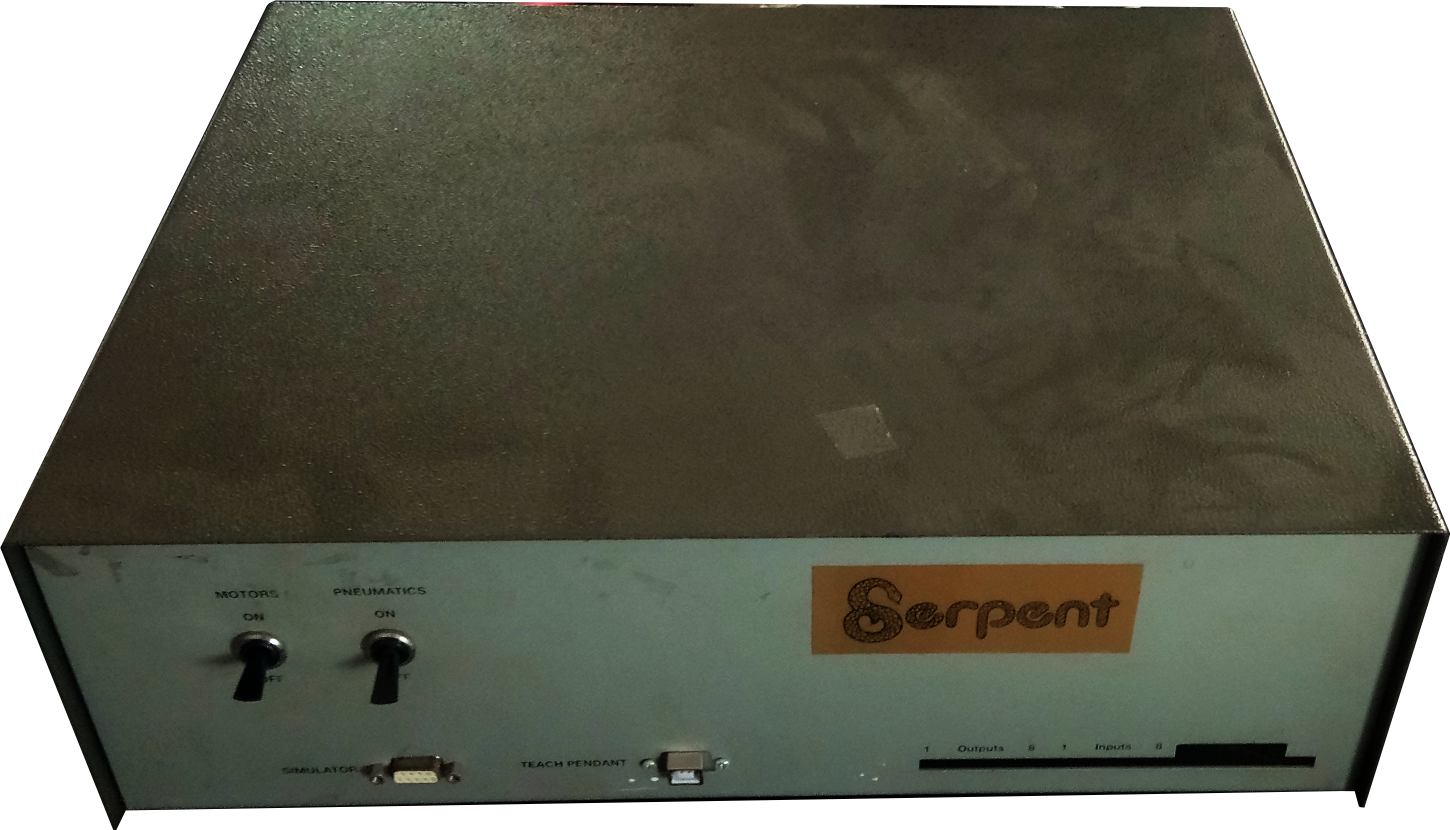
\includegraphics[width=9cm]{gambar/boxpanel.png}
	\caption{Box Panel Robot SCARA}
	\label{pic.boxpanel}
\end{figure}

Pada  SCARA menggunakan penggerak berupa motor DC 12 Volt dilengkapi dengan \textit{gearbox} sehingga mampu mengangkat beban berat karena torsi pada motor bertambah besar. Motor DC dikontrol oleh \textit{driver} motor EMS 30A H-\textit{Bridge} melalui Arduino Mega 2560. Spesifikasi dari motor DC yang digunakan pada robot SCARA ditunjukkan pada Tabel \ref{tbl.spesifikasimotordc}.
	\begin{table}[H]
	\centering
	\caption{Spesifikasi Motor DC pada Robot SCARA}
	\label{tbl.spesifikasimotordc}
	\resizebox{15cm}{!}{%
		\begin{tabular}{|l|l|}
			\hline
			\rowcolor[HTML]{9B9B9B} 
			\multicolumn{1}{c|}{\cellcolor[HTML]{9B9B9B}Keterangan}		& \multicolumn{1}{c|}{\cellcolor[HTML]{9B9B9B}Nilai}			\\ \hline
			Momen inersia lengan utama ($J_{1}$)    							& $0.0980kgm^{2}$ 				\\ \hline
			Momen inersia lengan depan ($J_{2}$)    							& $0.0115 kgm^{2}$ 				\\ \hline
			Massa lengan utama	($m_{1}$)											& $1.90kg$   					\\ \hline
			Massa lengan depan  ($m_{2}$)     										& $0.93kg$   					\\ \hline
			Momen inersia motor ($J_{m}$)      								& $3.3*10^{-6}kgm^{2}$ 			\\ \hline
			GGL untuk motor lengan utama dan motor lengan depan ($K_{e1}=K_{e2}$)  		& $0.047Nm/A$   				\\ \hline
			Resistansi jangkar motor lengan utama dan lengan depan($R_{a1}=R_{a2}$)		& $3.5\Omega$  					\\ \hline
			Induktasnis jangkar motor lengan utama dan lengan depan  ($L_{a1}=L_{a2}$) 		& $1.3mH$ 						\\ \hline
		\end{tabular}%
	}
\end{table}
%%
Pada bagian \textit{gearbox} pada masing-masing motor DC terdapat \textit{potensiometer} sebagai sensor posisi. Potensiometer ditempatkan pada bawah motor DC yang terhubung langsung. Setiap pergerakan dari motor DC, \textit{potensiometer} secara otomatis ikut bergerak dan kemudian mengirimkan nilai data analog ke Arduino Mega 2560. Data yang berhasil diterima oleh Arduino Mega 2560 kemudian diolah dan mendapatkan hasil berupa besar sudut pada pergerakan \textit{joint} tersebut. Bentuk fisik dari motor DC serta pemasangan \textit{potensiometer} ditunjukkan pada Gambar \ref{pic.potensiometer}.
\begin{figure}[H]
	\centering
	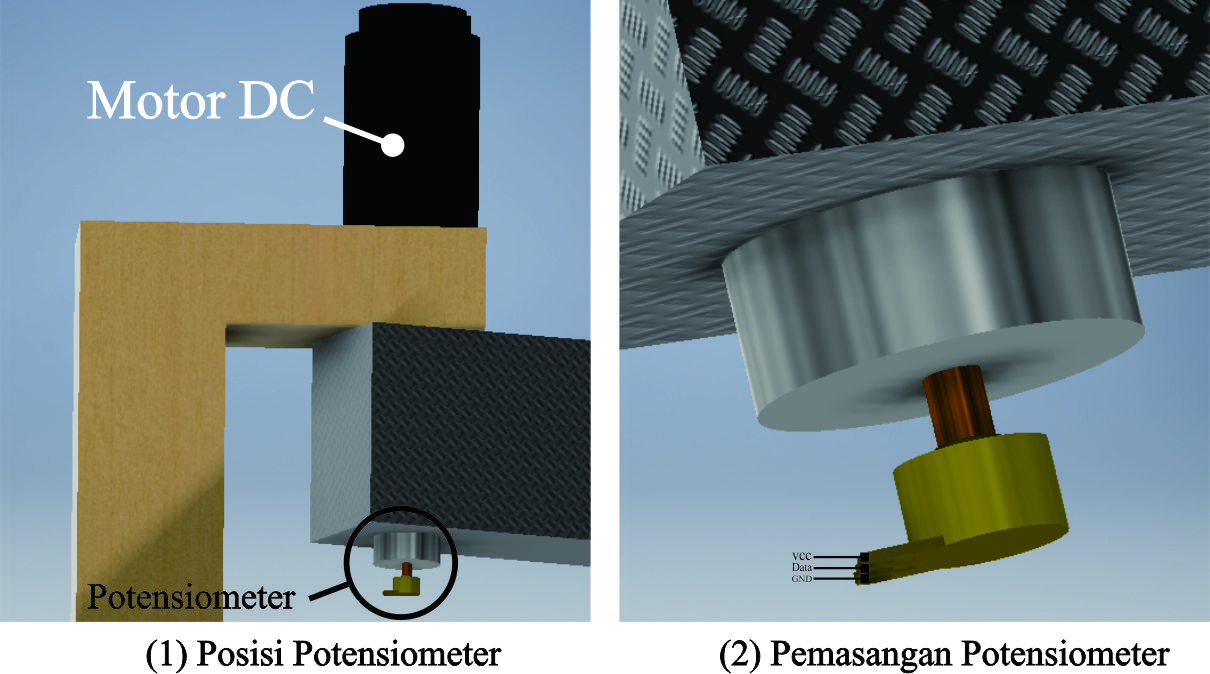
\includegraphics[width=12cm]{gambar/potsementara.jpg}
	\caption{Motor DC dengan potensiometer}
	\label{pic.potensiometer}
\end{figure}

Pada bagian \textit{end-effetor} menggunakan pergerakan translasi. Pergerakan translasi pada robot \textit{end-effector} merupakan gerak translasi pada sumbu Y. Pada robot SCARA pergerakan ini ada pada bagian \textit{end-effector} yang bergerak secara vertikal atau naik turun. Dengan pergerakan ini posisi \textit{end-effector} mengalami perubahan pada posisi tingginya. Pergerakan translasi juga terdapat pada bagian \textit{end-effector} yang menyebabkan sebuah \textit{gripper }\textit{ end-effector} dapat membuka dan menutup karena sebuah sistem mekanik yang telah ada di dalamnya. Selain dari pergerakan translasi, pergerakan pada \textit{end-effector} juga terdapat rotasi. Pergerakan ini dilakukan oleh satu buah motor DC yang ditempatkan pada bagian \textit{shoulder} dengan dihubungkan melalui sebuauh \textit{belt}. Pengoperasian pada motor DC ini juga dilakukan oleh \textit{driver} motor EMS 30A H-\textit{Bridge}. Bentuk fisik dari \textit{end-effector} pada robot SCARA ditunjukkan pada Gambar \ref{pic.endeffectorfisik}.
\begin{figure}[H]
	\centering
	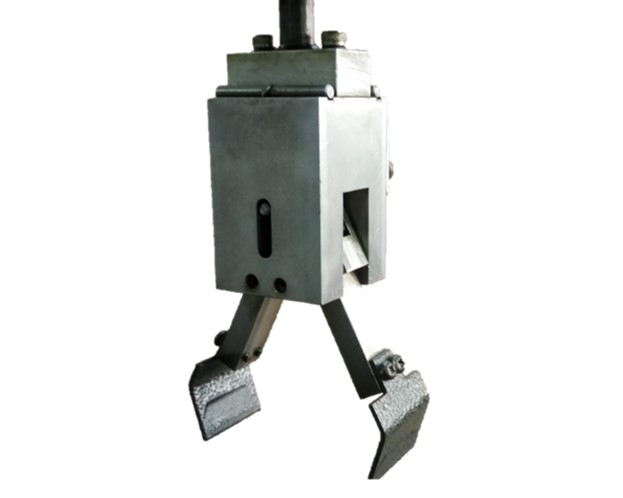
\includegraphics[width=6cm]{gambar/capitsementara.jpg}
	\caption{\textit{End-Effector} Robot SCARA}
	\label{pic.endeffectorfisik}
	
\end{figure}
Semua pergerakan pada \textit{end-effector} ditenagai oleh sebuah tekanan udara yang bersumber dari sebuah kompresor. Tekanan udara diaplikasikan pada sebuah \textit{pneumatic} dengan sistem kerja translasi yang dapat menyebabkan sebuah objek dapat bergerak pada sebuah garis lurus. Bentuk fisik dari \textit{pneumatic} robot SCARA ditunjukkan pada Gambar \ref{pic.pneumatic}.
\begin{figure}[H]
	\centering
	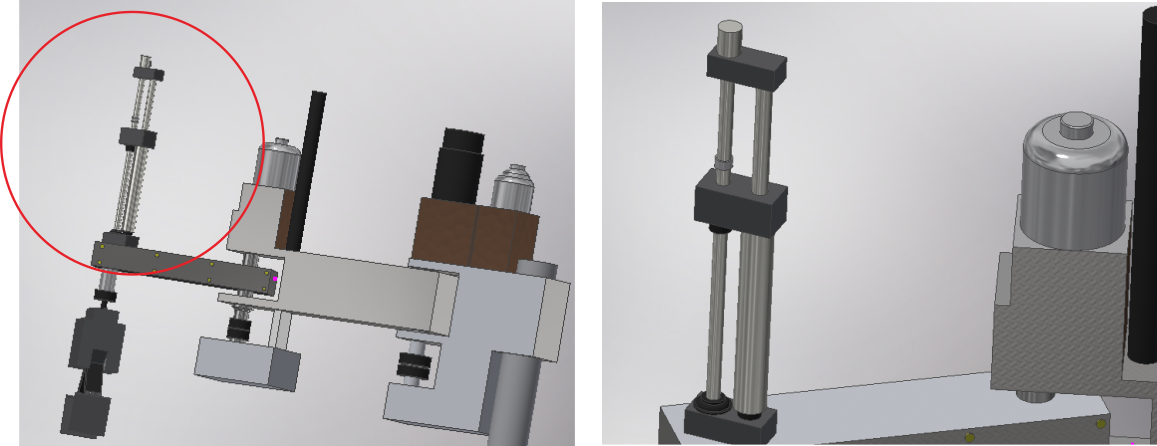
\includegraphics[width=12cm]{gambar/pneumatic.png}
	\caption{Bentuk Fisik \textit{Pneumatic}}
	\label{pic.pneumatic}
\end{figure}
Kompresor yang digunakan untuk menghasilkan sebuah tekanan udara merupakan sebuah kompresor listrik dengan kapasitas delapan bar. Kompresor ini dioperasikan menggunakan sumber tegangan AC 220 Volt. Ketika kapasitas udara sudah terpenuhi kompresor ini dapat digunakan tanpa menggunakan sumber tegangan tetapi hanya sebatas kapasitas udara yang disimpan. Bentuk fisik dari kompresor yang digunakan ditunjukkan pada Gambar \ref{pic.kompresor}.
\begin{figure}[H]
	\centering
	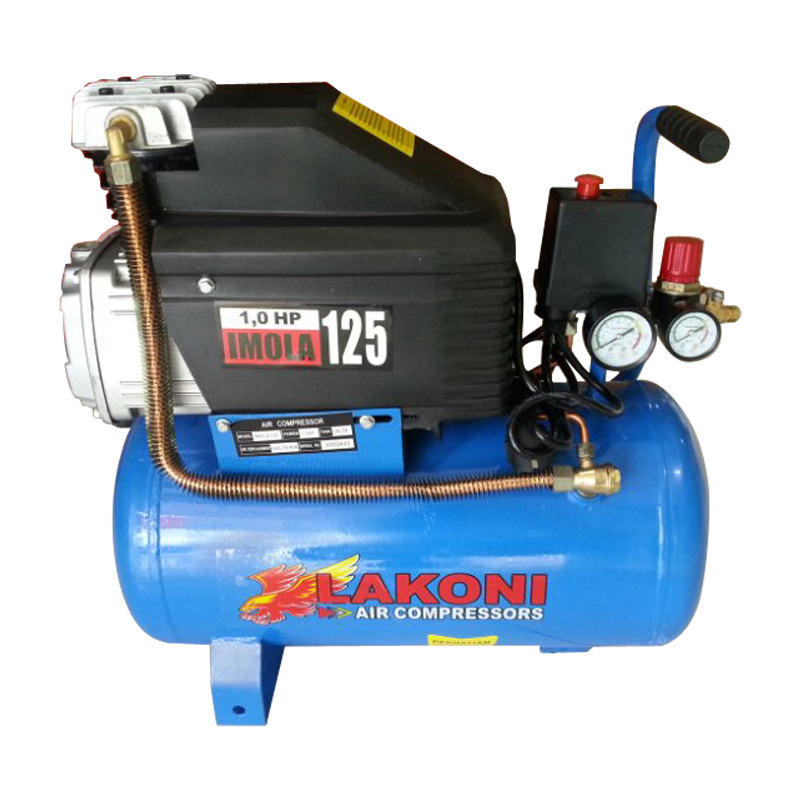
\includegraphics[height=5cm]{gambar/kompresor.png}
	\caption{Bentuk Fisik Kompresor}
	\label{pic.kompresor}
\end{figure}

Rancangan robot secara keseluruhan ditampilan pada Gambar \ref{pic.scarasamping} yang merupakan rancangan tampak samping dan Gambar \ref{pic.scaradimensi} merupakan rancangan dimensi robot. 
\begin{figure}[H]
	\centering
	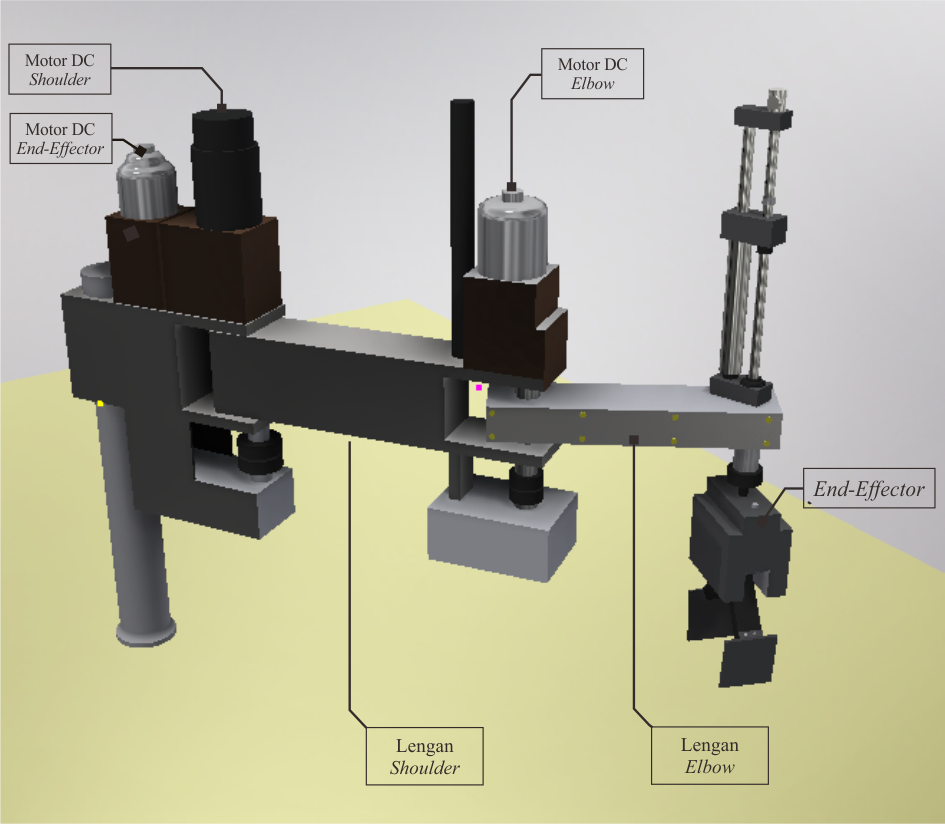
\includegraphics[height=9cm]{gambar/samping.png}
	\caption{Rancangan Tampak Samping}
	\label{pic.scarasamping}
\end{figure}

\begin{figure}[H]
	\centering
	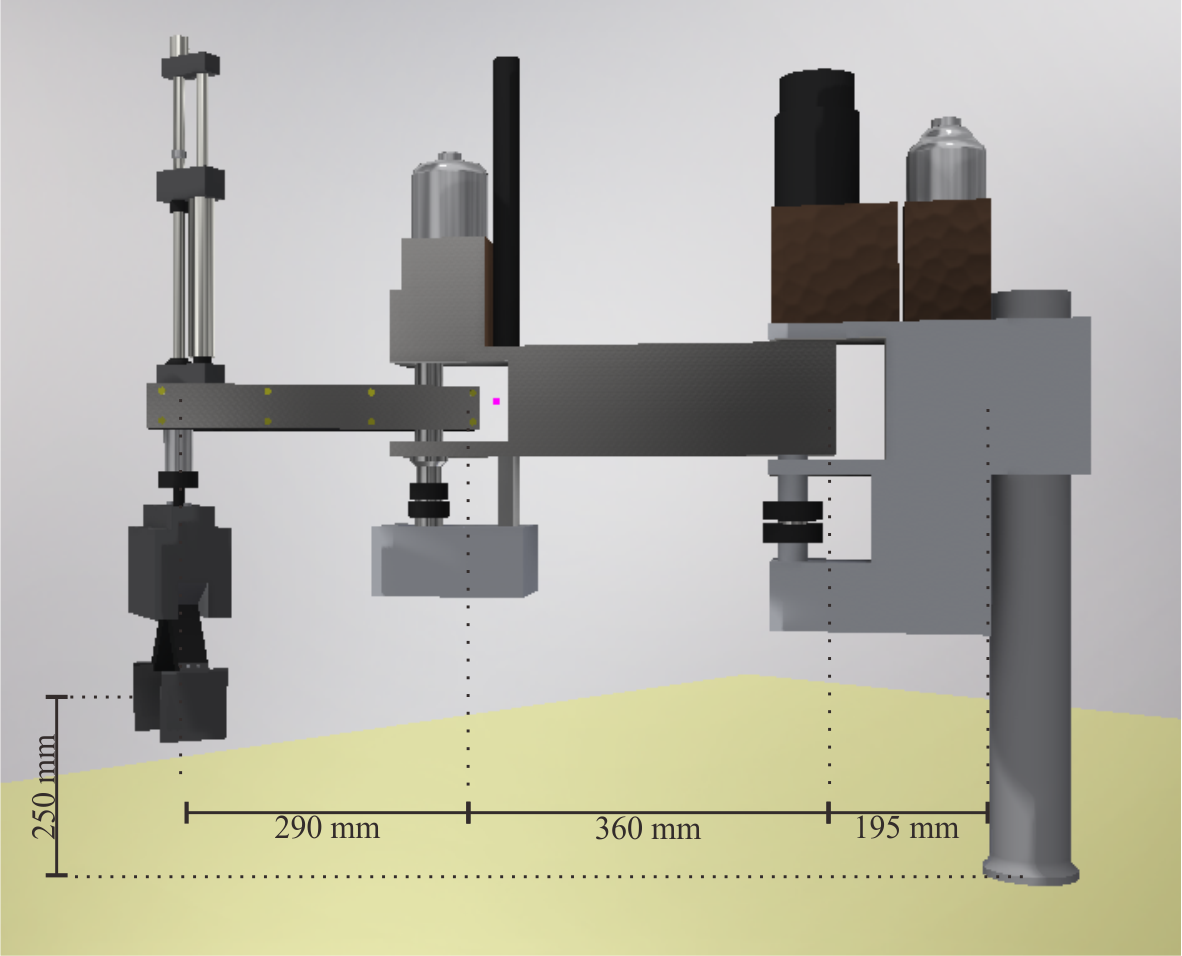
\includegraphics[height=9 cm]{gambar/scaradimensi.png}
	\caption{Dimensi Robot}
	\label{pic.scaradimensi}
\end{figure}

\subsection{Rangkaian Elektronika}
\subsubsection{Rangkaian Motor DC}
Rancangan kendali pada robot lengan SCARA ini menggunakan tiga buah motor DC dengan masing – masing dilengkapi dengan \textit{gearbox} untuk memperkuat torsi yang dihasilkan oleh motor DC. Pada  \textit{gearbox} masing – masing motor  DC diberikan sensor potensiometer sebagai \textit{feedback} untuk memberikan posisi motor DC pada keseluruhan sistem. Motor DC diletakkan pada \textit{shoulder} untuk \textit{end-effector} satu buah yang dihubungkan melalui \textit{belt}, pada \textit{shoulder} satu buah, dan pada \textit{elbow} satu buah. Ketiga motor DC tersebut masing-masing menggunakan \textit{driver} motor EMS 30A H-\textit{Bridge} dalam sistem kerjanya. Pada masing – masing motor DC membutuhkan catu daya 12 Volt DC. Rangkaian \textit{driver} motor mendapat sumber tegangan DC 12V untuk disalurkan ke pada motor DC dan 5 Volt untuk kerja dari \textit{driver} motor sendiri. Tegangan keluaran sebesar 12 Volt yang dihasilkan oleh regulator \textit{buck} dengan sumber dari tegangan DC 24 Volt setelah dilakukan \textit{converter} AC to DC. Gambar \ref{pic.motordcdriver} merupakan rangkaian motor DC, \textit{driver} motor, dan Arduino Mega 2560.  

\begin{figure}[H]
	\centering
	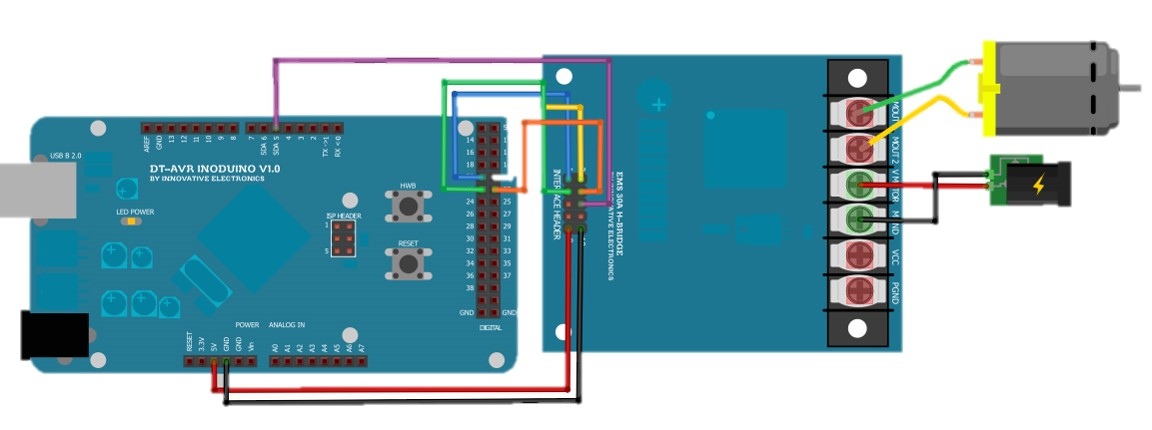
\includegraphics[width=10cm]{gambar/drivermotor.jpg}
	\caption{Rangkaian Arduino Mega 2560, \textit{Driver} Motor dan Motor DC}
	\label{pic.motordcdriver}
\end{figure}
\subsubsection{Rangkaian \textit{Valve Pneumatic}}
\textit{End-effector} menggunakan tekanan udara dalam melakukan pergerakannya. Tekanan udara ini dikontrol menggunakan sebuah \textit{valve relay}. \textit{Valve relay} yang digunakan dapat mengkontrol tekanan udara hingga delapan bar. \textit{Valve relay} dapat bekerja pada tegangan DC 24 Volt. Tegangan 24 Volt pada \textit{valve relay} didapat dari keluaran dari rangkaian AC-DC yang dilakukan oleh dioda \textit{bridge} dengan masukan awalnya adalah tegangan AC 24 Volt yang diberikan oleh sebuah tranformator. Dengan besaran tegangan 24 Volt maka sebuah Arduino tidak dapat mengkontrolnya. Oleh karena itu, diberi sebuah rangkaian pembantu yang prinsipinya bekerja seperti saklar. Rangkaian tersebut dikontrol oleh IC TIP31 yang nantinya  menerima sinyal data digital dari Arduino Mega 2560 dan akan membuka jalur untuk tegangan 24 Volt. Gambar \ref{pic.fisikvalve} merupakan bentuk fisik dari \textit{valve relay} yang digunaakan dan Gambar \ref{pic.skematikvalve} merupakan rangkaian dari \textit{valve pneumatic} dengan rangkaian TIP31.
\begin{figure}[H]
	\centering
	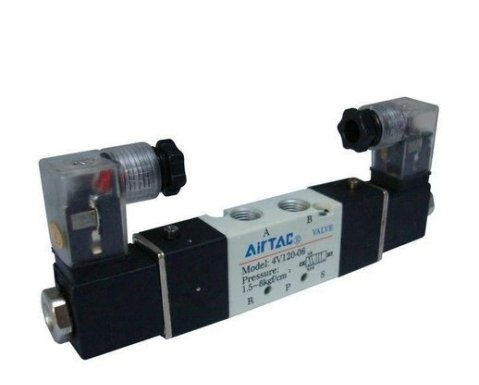
\includegraphics[width=5cm]{gambar/relay.jpg}
	\caption{Bentuk Fisik dari \textit{Valve Pneumatic}}
	\label{pic.fisikvalve}
\end{figure}
\begin{figure}[H]
	\centering
	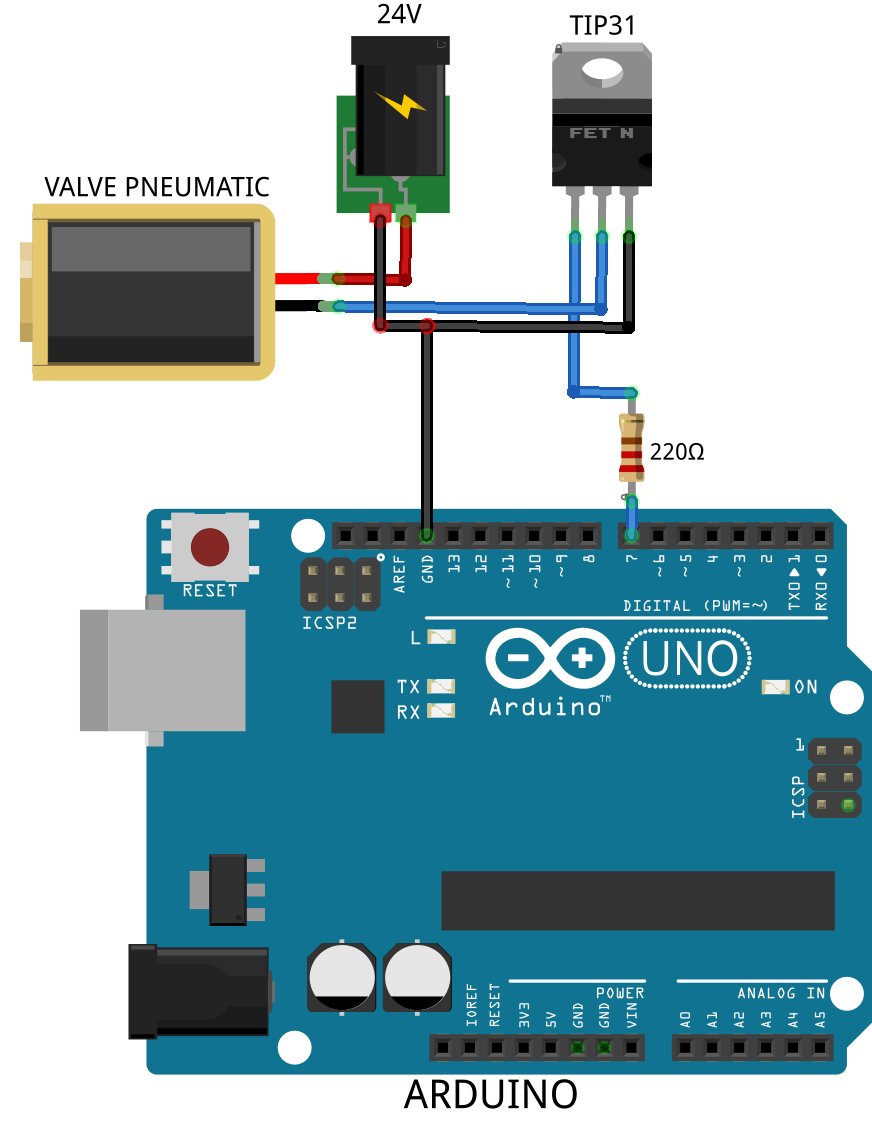
\includegraphics[width=5cm]{gambar/tip31.png}
	\caption{Rangkaian \textit{Valve Pneumatic} dengan Rangkaian TIP31}
	\label{pic.skematikvalve}
\end{figure}
\subsubsection{Sistem Elektronis Robot SCARA}
Arduino Mega 2560 digunakan sebagai mikrokontroler utama untuk mengendalikan seluruh sistem pada robot lengan SCARA. Arduino Mega 2560 memiliki banyak pin keluaran dan masukan digital dan analog yang dapat digunakan sebagai pengendali fungsi – fungsi dari setiap komponen. Pin pada Arduino  2560 dapat mencukupi kebutuhan masukan dan keluaran untuk sistem kerja robot. Pin \textit{analog} yang pada Arduino Mega 2560 digunakan untuk menerima \textit{feedback} masukkan dari \textit{potensiometer} yang ada pada setiap motor. Beberapa pin digital pada Arduino Mega 2560 juga  memiliki fungsi lain yaitu sebagai pin \textit{pulse with modulation} (PWM) yang dapat digunakan sebagai keluaran analog sehingga dapat digunakan untuk mengatur nilai tegangan kaluaran dari Arduino  2560. Pin PWM yang cukup digunakan untuk kontrol kecepatan pada \textit{driver} motor. Selain itu pin PWM pada Arduino Mega 2560 digunakan untuk memberikan kontrol direksi pada \textit{driver} motor untuk memberikan masukan arah putar kanan ataupun putar kiri. Gambar \ref{pic.boxpanelkabel} merupakan sistem elektronis keseluruhan robot SCARA yang terdapat di dalam \textit{box} panel dan Tabel \ref{tbl.elektronisscara} merupakan keterangan dari masing-masing komponen.
\begin{figure}[H]
	\centering
	\includegraphics[width=13cm]{gambar/panelkabel.png}
	\caption{Sistem Elektronis Robot SCARA}
	\label{pic.boxpanelkabel}
\end{figure}
% Please add the following required packages to your document preamble:
% \usepackage[table,xcdraw]{xcolor}
% If you use beamer only pass "xcolor=table" option, i.e. \documentclass[xcolor=table]{beamer}
% \usepackage{longtable}
% Note: It may be necessary to compile the document several times to get a multi-page table to line up properly
\begin{longtable}{|c|l|}
	\caption{Sistem Elektronis SCARA}
	\label{tbl.elektronisscara}\\
	\hline
	\rowcolor[HTML]{9B9B9B} 
	No & \multicolumn{1}{c|}{\cellcolor[HTML]{9B9B9B}Keterangan} \\ \hline
	\endfirsthead
	%
	\endhead
	%
	1  & \textit{Conncetor} utama                                          \\ \hline
	2  & Kipas                                                     \\ \hline
	3  &\textit{Valve relay pneumatic}                                   \\ \hline
	4  &\textit{Switch} motor dan \textit{pneumatic}                              \\ \hline
	5  & \textit{Connector remote  }                                      \\ \hline
	6  & \textit{Connector} Arduino Mega 2560                             \\ \hline
	7  & \textit{Board} utama                                             \\ \hline
	8  & \textit{Driver} motor EMS 30A H-\textit{Brdige}                           \\ \hline
	9  & Transformator                                           \\ \hline
	10 & \textit{Swtich} AC                                               \\ \hline
	11 & \textit{Connector} AC                                            \\ \hline
\end{longtable}

Pada Gambar \ref{pic.boxpanelkabel} terlihat bahwa sistem elektronis dari robot SCARA mempunyai kontrol utama yang terdiri dari Arduino Mega 2560 dan terdapat beberapa komponen pendukung. Gambar \ref{pic.sisminarduino} merupakan rangkaian elektronis utama dari robot SCARA yang disajikan melalui 3D Fusion dan Tabel \ref{tbl.pinarduino} merupakan fungsi dari masing-masing pin Arduino Mega 2560.
\begin{figure}[H]
	\centering
	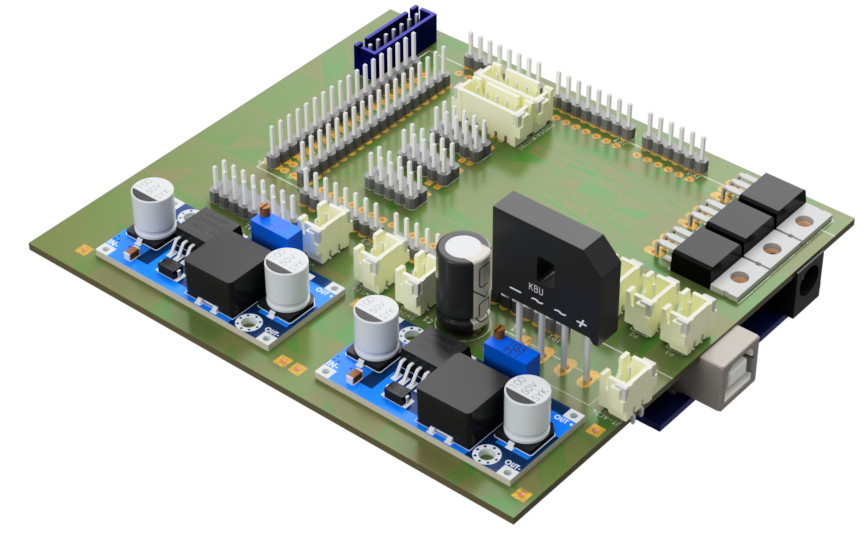
\includegraphics[width=10cm, height=10cm]{gambar/fusion.png}
	\caption{3D Fusion Rangkaian Elektronis}
	\label{pic.sisminarduino}
\end{figure}

% Please add the following required packages to your document preamble:
% \usepackage[table,xcdraw]{xcolor}
% If you use beamer only pass "xcolor=table" option, i.e. \documentclass[xcolor=table]{beamer}
% \usepackage{longtable}
% Note: It may be necessary to compile the document several times to get a multi-page table to line up properly
\begin{longtable}{|c|c|l|}
	\caption{Fungsi Arduino Mega 2560}
	\label{tbl.pinarduino}\\
	\hline
	\rowcolor[HTML]{656565} 
	{\color[HTML]{000000} No} & {\color[HTML]{000000} Pin Arduino} & \multicolumn{1}{c|}{\cellcolor[HTML]{656565}{\color[HTML]{000000} Fungsi}} \\ \hline
	\endfirsthead
	%
	\endhead
	%
	1                         & A1                                 & \textit{Feedback} potensiometer \textit{shoulder}                                            \\ \hline
	2                         & A2                                 & \textit{Feedback} potensiometer \textit{elbow}                                               \\ \hline
	3                         & A3                                 & {\color[HTML]{000000} \textit{Feedback} potensiometer \textit{end-effector}}                 \\ \hline
	4                         & D16, D18                           & Kontrol aktif \textit{driver} motor \textit{shoulder}                                        \\ \hline
	4                         & D20, D22                           & Kontrol \textit{driver} motor \textit{shoulder}                                              \\ \hline
	5                         & D24, D26                           & Kontrol aktif \textit{driver} motor \textit{elbow}                                           \\ \hline
	6                         & D28. D30                           & Kontrol \textit{driver} motor \textit{elbow}                                                 \\ \hline
	7                         & D32, D34                           & Kontrol aktif \textit{driver} motor \textit{end-effector  }                                  \\ \hline
	8                         & D36, D38                           & Kontrol \textit{driver} motor \textit{end-effector }                                         \\ \hline
	9                         & D4                                 & Kontrol PWM \textit{driver} motor \textit{shoulder}                                          \\ \hline
	10                        & D5                                 & Kontrol PWM \textit{driver} motor \textit{elbow}                                             \\ \hline
	11                        & D6                                 & Kontrol PWM \textit{driver} motor \textit{end-effector}                                      \\ \hline
	12                        & D7                                 & Kontrol \textit{valve relay} naik                                                   \\ \hline
	13                        & D8                                 & Kontrol \textit{valve relay} turun                                                  \\ \hline
	14                        & D9                                 & Kontrol \textit{valve relay} buka-tutup                                             \\ \hline
	15                        & D15                                & Kontrol LED \textit{Shoulder} aktif \textit{high}                                            \\ \hline
	16                        & D17                                & Kontrol LED \textit{elbow} aktif \textit{high}                                               \\ \hline
	17                        & D19                                & Kontrol LED \textit{end-effector} naik aktif \textit{high}                                   \\ \hline
	18                        & D21                                & Kontrol LED \textit{end-effector} turun aktif \textit{high}                                  \\ \hline
	19                        & D23                                & Kontrol LED \textit{end-effector} buka-tutup aktif \textit{high}                             \\ \hline
	20                        & D25                                & Buzzer aktif \textit{high}                                                          \\ \hline
\end{longtable}

\subsubsection{Rangkaian Catu Daya}
Rangkaian catu daya merupakan hal yang sangat penting dalam sebuah sistem. Pada robot lengan SCARA terdapat tiga buah nilai tegangan \textit{supply} yang berbeda. Tegangan yang ditujukkan untuk Arduino Mega 2560 dan beberapa sensor membutuhkan tegangan 5 Volt, motor DC membutuhkan tegangan 12 Volt dan \textit{valve pneumatic} membutuhkan tegangan 24 Volt. Catu daya diawali dengan tegangan AC 220 Volt dari listrik PLN. Tegangan tersebut kemudian diturunkan menggunakan sebuah trafo 5 Ampere menjadi 24 Volt AC. Komponen yang digunakan dalam rangkaian merupakan komponen yang membutuhkan tegangan DC, maka tegangan 24 Volt AC diubah menjadi 24 Volt DC menggunakan rangkaian dioda \textit{bridge}. Tegangan 24 Volt DC diarahkan menuju dua buah regulator \textit{buck} LM2596 yang masing-masing menghasilkan tegangan 12 Volt dan 5 Volt. Rangkaian catu daya secara keseluruhan ditunjukkan pada Gambar \ref{pic.skematikcatu}.
\begin{figure}[H]
	\centering
	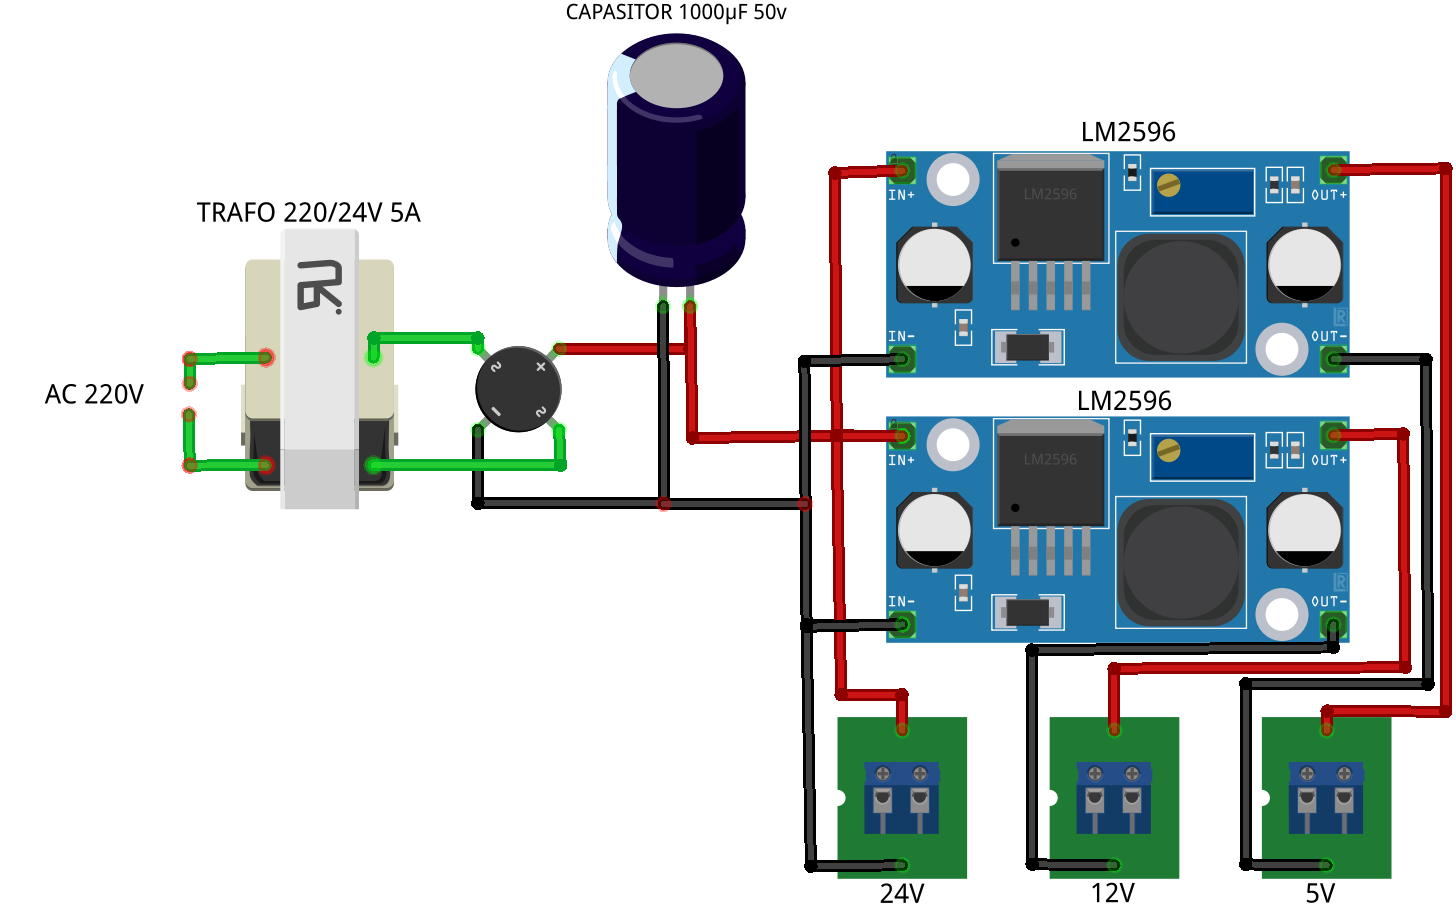
\includegraphics[width=8cm]{gambar/catudaya_bb.png}
	\caption{Rangkaian Catu Daya}
	\label{pic.skematikcatu}
\end{figure}
\section{Perancangan Perangkat Lunak}
Perangkat lunak yang digunakan merupakan \textit{software} Processing IDE. Processing IDE diprogram agar menghasilkan sebuah GUI yang cocok sesuai dengan fungsi robot SCARA. Di dalam GUI terdapat dua bagian yang diantaranaya merupakan bagian \textit{control} dan bagian \textit{display}. Pada bagian kontrol pada GUI berfungsi untuk mengkontrol mulai dari pergerakan dan posisi dari robot SCARA. Sedangkan pada bagian penampil, GUI menampilkan nilai dari sudut, posisi, serta animasi terkait robot SCARA. Gambar \ref{pic.gui} merupakan tampilan dari GUI secara keseluruhan. Setiap komponen yang ditampilan di dalam GUI processing IDE ditunjukkan pada Tabel \ref{tbl.gui}.
\begin{figure}[H]
	\centering
	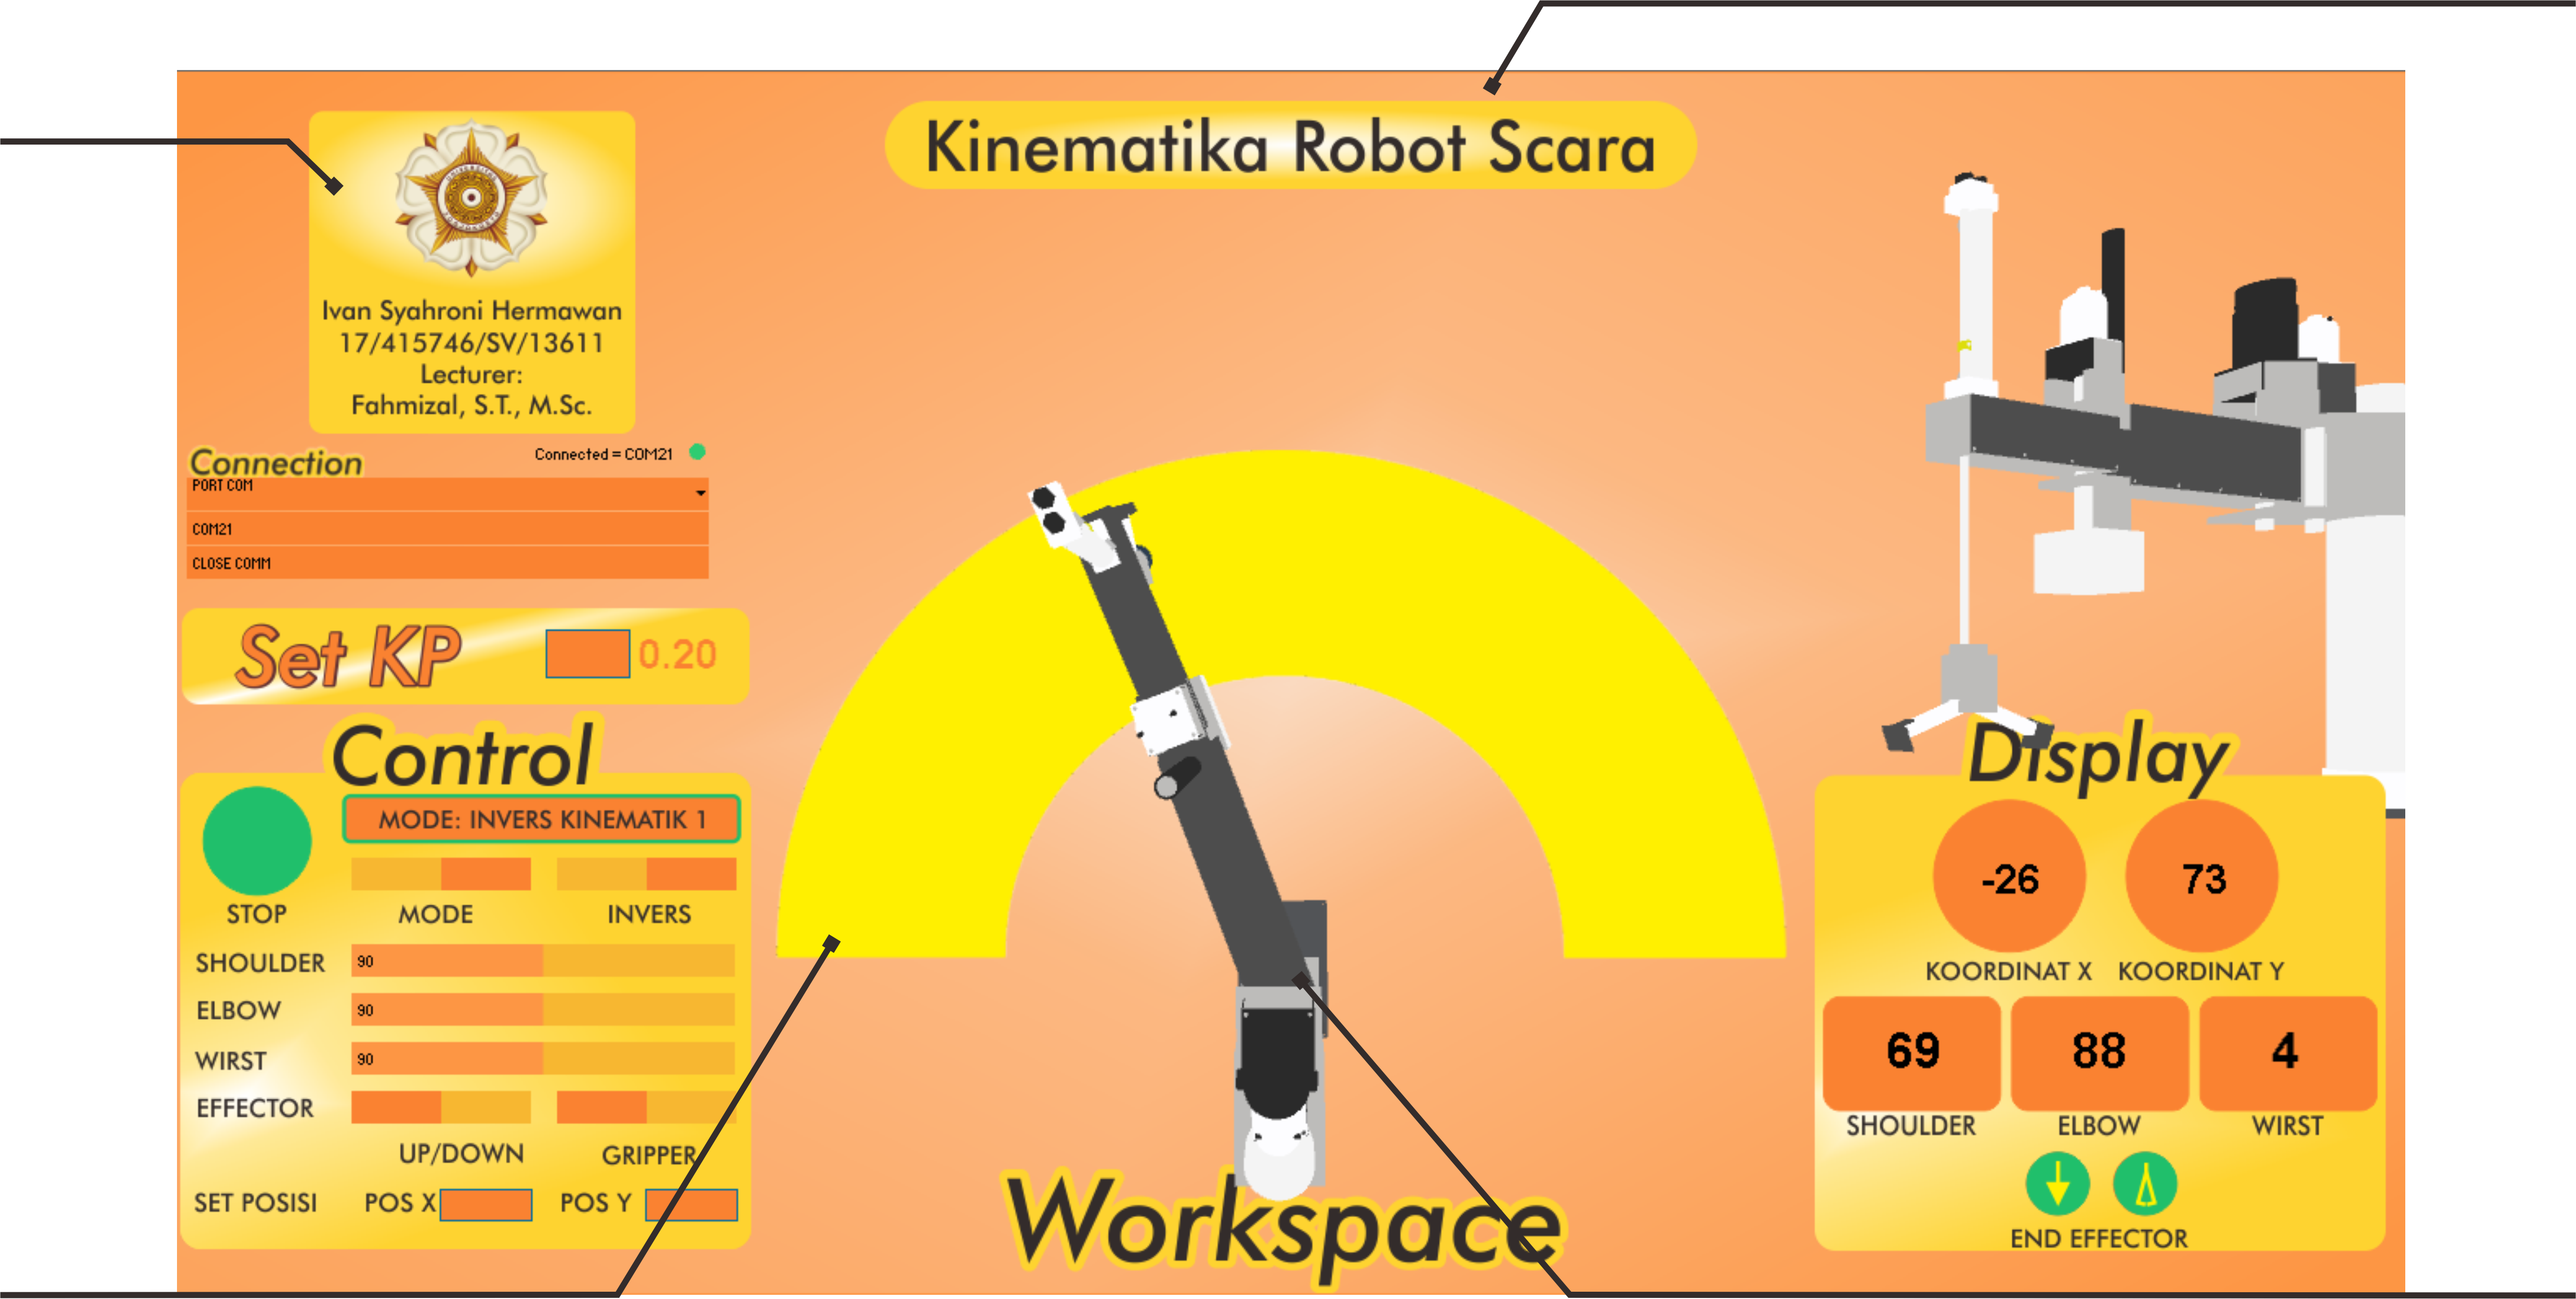
\includegraphics[width=15cm ]{gambar/GUI.png}
	\caption{Tampilan GUI Sistem Kinematika Robot SCARA}
	\label{pic.gui}
\end{figure}

\begin{table}[H]
	\centering
	\caption{Keterangan Tampilan pada GUI Robot SCARA}
	\label{tbl.gui}
	\small
	\begin{tabular}{|c|l|l|}
		\hline
		\rowcolor[HTML]{9B9B9B} 
		No & \begin{tabular}[c]{@{}c@{}}Nama\end{tabular} & \multicolumn{1}{c|}{\cellcolor[HTML]{9B9B9B}Fungsi} \\ \hline
		1  &	Identitas& Menampilkan identitas                   \\ \hline
		2  & Koneksi& Menentukan komunikasi dengan \textit{hardware} yang akan dihubungkan                        \\ \hline
		3  & Set kendali proposional& Memasukkan nilai kendai proposional                 \\ \hline
		4  & Kelompok \textit{control}& Terdiri dari beberapa kontrol untuk mengatur pergerakan robot SCARA              \\ \hline
		5  & \textit{Workspace}& Ruang kerja robot SCARA              \\ \hline
		6  & \textit{3D Shape} tampak atas & Menampilkan pergerakan robot SCARA tampak atas                  \\ \hline
		7  & Kelompok \textit{display} & Menanmpilkan data-data terkait robot SCARA          \\ \hline
		8  &\textit{3D Shape} tampak samping & Menampilkan pergerakan robot SCARA tampak samping                  \\ \hline
		9  & Judul &  Judul dari antarmuka robot SCARA                \\ \hline
	\end{tabular}
\end{table}


\subsection{ControlP5}
ControlP5 merupakan salah satu \textit{library} yang berguna dalam membuat sebuah GUI. Dalam \textit{library} yang disediakan terdapat banyak pilihan terkait kontrol sistem yang dapat digunakan. Kontrol sistem yang disediakan tersedia dua pilihan yaitu untuk menkontrol dan untuk menampilkan sebuah data. Masing-masing kontrol sistem ini dapat digunakan dengan cara memanggilnya pada program yang ditulis.

Pada perancangan kinematika robot SCARA ini, menggunakan empat buah kontrol sistem. Empat kontrol sistem yang digunakan merupakan jenis kontrol sistem yang berguna untuk memberikan sebuah data yang dikirimkan pada Arduino Mega 2560. Kontrol sistem tersebut diantaranya:
\begin{enumerate}
	\item \textit{Slider Control} \\
	\textit{Slider Control} berupa tampilan kontrol GUI yang menggunakan sistem geser dalam memberikan data. Data memiliki batasan atas dan batas bawah yang dimasukkan dalam program. Keuntungan menggunakan kontrol sistem jenis ini adalah mudahnya dalam memberikan sebuah data yang berbeda.


	\item \textit{Textfield Control} \\
\textit{Textfield control} berupa tampila kontrol GUI yang menggunakan masukan nilai data sesuai apa yang dituliskan atau diketikkan secara langsung. Kelebihan menggunakan kontrol sistem jenis ini karena dapat memasukkan nilai data lebih spesifik secara langsung sesuai keiinginan.
	

	\item \textit{Toggle Control} \\
\textit{Toggle control}
\textit{Toggle control} memiliki sistem kontrol seperti saklar ON-OFF. Pada saat ditekan maka \textit{toggle control} menyimpan data berupa kondisi pertama dan berubah saat ditekan kembali. 

\end{enumerate}
\subsection{\textit{Shape}}
\textit{Shape} pada GUI berfungsi sebagai penampil animasi tiga dimensi dari robot SCARA. Robot SCARA dapat ditampilkan dalam berbagai ukuran, letak dan juga dapat bergerak sesuai dengan data yang diberikan. Pergerakan dari robot SCARA merupakan implementasi dari wujud aslinya dengan pergerakan yang sama. Dalam pengoperasianya, desain dari robot SCARA yang ditampilkan harus dimasukkan ke dalam folder yang sama dengan program Processing IDE. File yang dapat ditampilkan merupakan file dengan jenis obj. yang berarti file objek. Pada program robot SCARA file dari dimensi tiga dari robot SCARA memiliki tiga buah file dimana ketiganya adalah \textit{base, shoulder}, dan \textit{elbow}. 

\section{Sistem Kinematika}
Persamaan kinematika terbagi dua, yaitu kinematika maju dan kinematika balik. Kinematika maju digunakan untuk menentukan posisi dan orientasi \textit{end-effector} apabila variabel sudut \textit{joint}-nya telah diketahui. Kinematika balik digunakan untuk mencari \textit{joint} robot dalam menentukan posisi dan orientasi dari \textit{end-effector.}
\subsection{Prinsip Kerja Kinematika Maju}
Metode Denavit-Hartenberg (DH) merupakan metode yang menggabungkan proses perhitungan rotasi dan translasi menjadi sebuah matriks yang menyertakan nilai-nilai sudut putar dan jarak sendi dari sebuah lengan robot. Dalam beberapa aplikasi, metode Denavit-Hartenberg umumnya digunakan dalam perhitungan \textit{forward kinematics}. Dalam penelitian ini dirancang aplikasi yang menggunakan metode Denavit-Hartenberg untuk menghitung sudut-sudut tiap sendi pada sebuah lengan robot. Matrik Denavit-Hartenberg yang berisi perhitungan rotasi dan translasi digunakan untuk mendapatkan nilai nilai sudut untuk menggerakkan tiap motor sendi. Empat aturan \textit{frame} Denavit-Hartenberg yaitu Sumbu $z$ harus menjadi sumbu rotasi atau translasi dari sebuah \textit{joint}. Sumbu $x$ harus tegak lurus dari sumbu $z$ \textit{frame} sebelumnya. Sumbu $x$ harus memotong atau menyilang dari sumbu $z$ \textit{frame} sebelumnya. Sumbu $y$ harus digambarkan sesuai dengan aturan tangan kanan setelah sumbu $x$   dan sumbu $z$ setiap \textit{frame} digambarkan. Gambar \ref{dhscara} merupakan struktur dari konfigurasi SCARA.
\begin{figure}[H]
	\centering
	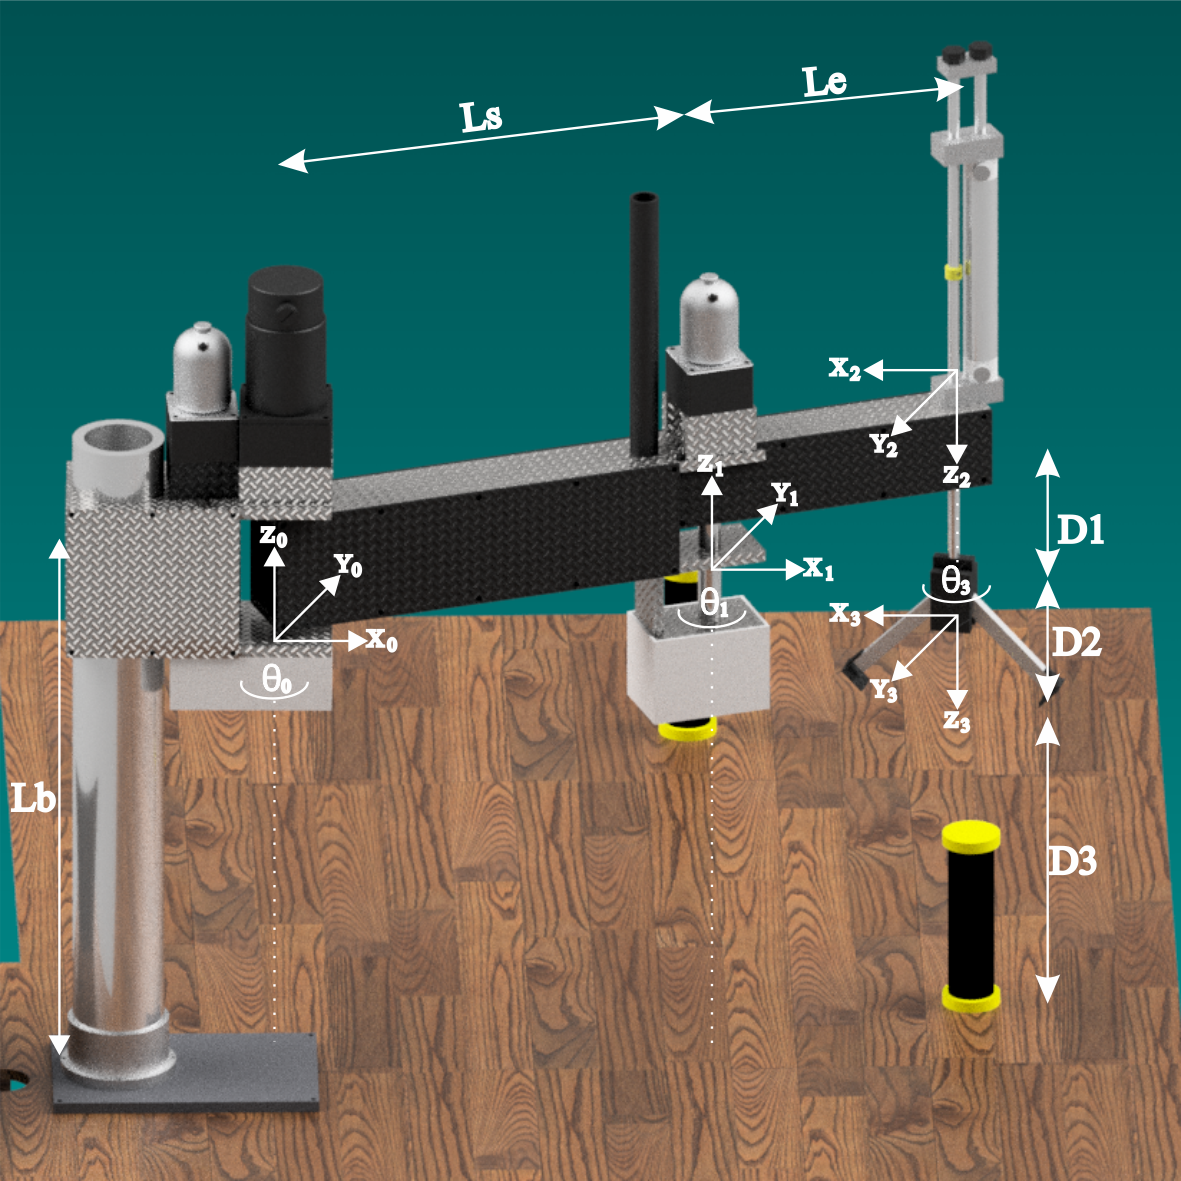
\includegraphics[width=9cm ]{gambar/scaradh.png}
	\caption{Konfigurasi Robot SCARA}
	\label{dhscara}
\end{figure}
Pada setiap \textit{joint} dari robot SCARA memiliki nomor dari 1 sampai 4 dengan digambarkan sebuah vektor $x, y, z$ pada masing-masing \textit{jointnnya} yang berfungsi untuk memudahkan dalam pengisian pada parameter DH. Vektor $x, y, z$ digambarkan sesuai dengan arah pergerakan pada masing-masing \textit{joint} dimana $z$ merupakan koordinat dari pergerakan \textit{joint} tersebut. Selanjutnya dengan mengikuti kaidah tangan kanan maka arah dari $x$ dan $y$ dapat diketahui. 

Pada saat vektor telah digambarkan pada keseluruhan \textit{joint}, langkah selanjutnya adalah menentukan parameter DH yang diawali dengan menentukan $\alpha_{i}. \alpha_{i}$ merupakan besar sudut yang terbentuk dari koordinat $z_{i}$ dengan $z_{i-1}$.  Dimulai pada \textit{joint} 1, $\alpha_{1}$ adalah 0 karena koordinat $z_{0}$ dan $z_{1}$ mempunyai arah yang sama sehingga sudut yang dihasilkan antara $z_{0}$ dan $z_{1}$ adalah 0.  Pada \textit{joint} 2 nilai pada $\alpha_{2}$ adalah 180 atau  $\pi$ karena arah dari  $z_{1}$ dan  $z_{2}$ mengarah ke arah yang berlawanan yang berarti memiliki sudut 180. Pada \textit{joint} 3 dan 4 memiliki nilai 0 karena koordinat $z_{2}$ dan $z_{3}$ dalam arah yang sama yang berarti tidak ada perbedaan sudut.

Pada langkah selanjutnya adalah menentukan nilai dari $a_{i}$ dan $d_{i}$. $a_{i}$ merupakan nilai panjang dari jarak koordinat  $z_{i}$  dan  $z_{i-1}$ . Sedangkan $d_{i}$ merupakan nilai panjang dari jarak koordinat $x_{i}$ dan $x_{i-1}$. Pada \textit{joint} 1 nilai dari $a_{1}$ adalah LS karena jarak antara $z_{1}$ dengan $z_{0}$ dapat direpresentasikan dengan panjang LS atau panjang dari lengan \textit{shoulder} dan untuk $d_{1}$ mempunyai nilai 0 karena koordinat $x_{0}$ dan $x_{1}$ tidak memiliki perbedaan pada sumbu $y$. Untuk \textit{joint} 2, nilai dari $a_{2}$ adalah Le atau lengan \textit{elbow} dikarenakan posisi dari koordinat $z_{1}$  dan $z_{2}$  memiliki jarak yang dapat direpresentasikan menjadi Le dan untuk  $d_{2}$ memiliki nilai 0 dikarenakan tidak ada perbedaan pada sumbu $y$ pada  $x_{1}$ dan  $x_{2}$.  Untuk \textit{joint} 3 memiliki $a_{3}$ memiliki nilai 0 karena koordinat $z$ berada pada sumbu yang sama sehingga tidak ada jarak dan untuk nilai $d_{3}$  memiliki nilai D1 karena jarak antara $x_{2}$ dan $x_{3}$ dapat direpresentasikan dengan D1 yang merupakan sebuah variabel. Untuk \textit{joint} terakhir yaitu \textit{joint} 4 nilai $a_{4}$ adalah 0 karena koordinat $z_{3}$ dan $z_{4}$ searah dan berada pada satu sumbu dan nilai dari $d_{4}$ adalah D2.

Langkah terakhir adalah menentukan nilai $\theta_{i}$ pada masing-masing \textit{joint} yang memiliki jenis \textit{joint}  \textit{revolute}. Pada robot SCARA \textit{joint revolute} berada pada \textit{joint} 1, \textit{joint} 2, dan \textit{joint} 4.  $\theta_{i}$ merupakan sebuah variabel yang nilainya dapat menyesuaikan kondisi dari robot. Nilai  $\theta_{i}$ ditempatkan pada koordinat $z_{i}$ yang merupakan sumbu dari setiap \textit{joint}. 

Setelah paramaeter DH telah ditentukan semuanya kemudian nilai-nilai dari masing-masing parameter dituliskan ke dalam bentuk tabel yang bertujuan untuk memudahkan saat akan dimasukkan ke dalam sebuah persamaan. Tabel parameter DH terdiri dari baris yang berisi tentang joint yang dimiliki oleh robot dan kolom yang merupakan parameter DH seperti $a_{i},\alpha_{i}, d_{1}, dan \theta_{i}$. Tabel parameter DH dari robot SCARA ditunjukkan pada Tabel \ref{dh.scara}. 

\begin{table}[H]
	\centering
	\caption{DH Parameter Robot SCARA}
	\label{dh.scara}

		\begin{tabular}{|c|c|c|c|c|}
			\hline
			\rowcolor[HTML]{9B9B9B} 
			Link & $a_{1}$ & $\alpha_{1}$ & $d_{1}$ & $\theta_{1}$ \\ \hline
			1    & LS & 0      & 0     & $\theta_{1}$     \\ \hline
			2    & LE & $\pi$    & 0     & $\theta_{2}	$     \\ \hline
			3    & 0     & 0      & D1 & 0          \\ \hline
			4    & 0     & 0      & D2 & $\theta_{4}$ \\ \hline
		\end{tabular}
	
\end{table}

Dari parameter DH yang ditunjukkan pada Tabel \ref{dh.scara} dapat diimplementasikan ke dalam sebuah transformasi matriks. Terdapat empat buah transformasi matriks yang masing-masing menunjukan dari pergerakan \textit{joint} yang kemudian dimasukkan ke dalam persaaama parameter DH. Persamaan \ref{pers.dhscara} merupakan persamaan utama dari metode DH yang dari persamaan tersebut dapat dikelompokkan menjadi empat transformasi matriks.
\begin{equation}
A_{1} = R_{z1\theta1}T_{z1d1}T_{x1a1}R_{x1\alpha1}
\label{pers.dhscara}
\end{equation}

Dari persaman \ref{pers.dhscara} dapat dibagi menjadi empat kelompok yang membentuk transformasi matriks. Ke empat transforamasi matriks ini di dapat dari matriks yang dimiliki oleh parameter DH seperti yang ditunjukkan pada Persamaan \ref{dh.full}. Ke empat matriks tersebut kemudian digabungkan dan membentuk satu buat transformasi matriks secara keseluruhan. Matriks secara keseluruhan digunakan dalam melakukan perhitungan kinematika maju.

\begin{equation}
A_{i} = \begin{bmatrix}
\cos\theta_{i} &  -\cos\alpha_{i}\sin\theta_{i}&  \sin\alpha_{i}\sin\theta_{i}& a_{1}\cos\theta_{i}\\ 
\sin\theta_{i}&  \cos\alpha_{i}\cos\theta_{i}&  -\sin\alpha_{i}\cos\theta_{i}& a_{1}\sin\theta_{i}\\ 
0&\sin\alpha_{i}  &\cos\alpha_{i}  &d_{1} \\ 
0 & 0 & 0 &1 
\end{bmatrix}
\label{dh.full}
\end{equation}

 Persamaan \ref{dh.scara1}, \ref{dh.scara2}, \ref{dh.scara3}, dan \ref{dh.scara4} merupakan transformasi matriks dari masing-masing \textit{joint} dengan nilai-nilai yang sudah dimasukkan sesuai dengan matriks pada Persamaan \ref{dh.full}. Pada ke empat matriks $C_{i}$ mempresentasikan $\cos\theta_{i}$ dan $S_{i}$ mempresentasikan $\sin\theta_{i}$.
\begin{equation}
A_{1} = \begin{bmatrix}
C_{1} &  -S_{1}&  0& a_{1}C_{1}\\ 
S_{1}&  C_{1}&  0& a_{1}C_{1}\\ 
0&0  &1  &0 \\ 
0 & 0 & 0 &1 
\end{bmatrix}
\label{dh.scara1}
\end{equation}

\begin{equation}
A_{2} = \begin{bmatrix}
C_{2} &  S_{2}&  0& a_{2}C_{2}\\ 
S_{2}&  -C_{2}&  0& a_{2}C_{2}\\ 
0&0  &-1  &0 \\ 
0 & 0 & 0 &1 
\end{bmatrix}
\label{dh.scara2}
\end{equation}


\begin{equation}A_{3}=\begin{bmatrix}
1 & 0 &0  &0 \\ 
0&1  &0  &0 \\ 
0 &0  &1  &d_{3} \\ 
0&0  &0  &1 
\end{bmatrix} 
\label{dh.scara3}
\end{equation}

\begin{equation}
A_{4} = \begin{bmatrix}
C_{4} &  -S_{4}&  0& 0\\ 
S_{4}&  C_{4}&  0& 0\\ 
0&0  &1  &d_{4} \\ 
0 & 0 & 0 &1 
\end{bmatrix}
\label{dh.scara4}
\end{equation}

Dari ke empat persamaan transformasi matriks dari rotasi dan translasi dari konfirgurasi robot SCARA, dapat digabungkan menjadi satu buah matriks secara keseluruhan. Persaman \ref{dh.scara5} merupakan persamaan akhir dari transformasi robot SCARA menggunakan metode parameter DH . Dengan persamaan ini, maka perhitungan untuk mencari sebuah besar \textit{joint} dapat diselesaikan.

\begin{equation}
\small
T_{4}^{0}=A_{1} ... A_{4} =
\begin{bmatrix}
C_{12}C_{4}S_{12}S_{4}&-C_{12}S_{4}+S_{12}c_{4}  & 0  & a_{1}C_{1}+a_{2}C_{12} \\ 
S_{12}C_{4}-C_{12}S_{4}&-S_{12}S_{4}-C_{12}C_{4} &0  &a_{1}S_{1}+a_{2}S_{12} \\ 
0 & 0 & -1 & -d_{3}-d_{4}\\ 
0 &0  &0  &1 
\end{bmatrix}
\label{dh.scara5}
\end{equation}

Dengan menggunakan matriks $T_{4}^{0}$ pada Persamaan \ref{dh.scara5} memungkinkan untuk menghitung nilai dari koordinat $P_{x}, P_{y}$ dan $P_{z}$. Nilai koordinat $P_{x}$ dapat ditentukan memalui Persamaan \ref{pers.x}. Nilai koordinat $P_{y}$ ditentukan melalui Persamaan \ref{pers.y} dan nilai koordinat $P_{z}$ ditentukan dengan Persamaan \ref{pers.z}. Nilai dari koordinat ini tergantung pada nilai konstan yang dimiliki pada robot SCARA dan beberapa kondisi dari pada variabel. Nilai konstan yang dimiliki dari robot SCARA ditunjukkan pada Tabel\ref{tbl.konstanscara}.

\begin{equation}
P_{x}=a_{1}C_{1}+a_{2}C_{12}
\label{pers.x}
\end{equation}

\begin{equation}
P_{y}=a_{1}S_{1}+a_{2}S_{12}
\label{pers.y}
\end{equation}

\begin{equation}
P_{z}=-d_{3}-d_{4}
\label{pers.z}
\end{equation}

\begin{table}[H]
	\centering
	\caption{DH Parameter Robot SCARA}
		\label{tbl.konstanscara}
	\begin{tabular}{|c|c|c|c|}
		\hline
		\rowcolor[HTML]{9B9B9B} 
		Parameter & Nilai & Parameter & Nilai  \\ \hline
		LS    & 360 mm & D1      & 105          \\ \hline
		LE    & 290 mm &D2    & 80       \\ \hline
		LB    & 360 mm     & D3      &150    \\ \hline

	\end{tabular}
	
\end{table}

Setelah nilai-nilai parameter dimasukkan kedalam Persamaan \ref{pers.x}, \ref{pers.y}, dan \ref{pers.z} maka pada setiap persamaan mengalami perbedaan. Nilai koordinat $P_{x}$ dapat ditentukan memalui Persamaan \ref{pers.x1}. Nilai koordinat $P_{y}$ ditentukan melalui Persamaan \ref{pers.y1} dan nilai koordinat $P_{z}$ ditentukan dengan Persamaan \ref{pers.z1}.

\begin{equation}
P_{x}=LS\cos\theta_{1}+LE\cos\theta{1+2}
\label{pers.x1}
\end{equation}

\begin{equation}
P_{y}=LS\sin\theta_{1}+LE\sin\theta{1+2}
\label{pers.y1}
\end{equation}

\begin{equation}
P_{z}=-D1-D4
\label{pers.z1}
\end{equation}

\subsection{Prinsip Kerja Kinematika Balik}
Kinematika balik adalah perhitungan untuk mencari variabel sudut (\textit{joint}) robot dalam menentukan posisi dan orientasi dari \textit{end-effector}. Dalam menentukan koordinat \textit{end-effector}, kinematika balik harus disesuaikan dengan batas area kerja \textit{(workspace)} dari jangkauan robot. Penyelesaian kinematika balik ini dapat diselesaikan dengan menggunakan hukum \textit{phytagoras} dan aturan \textit{cosinus}. 
Secara garis besar metode kinematika balik akan mencari nilai parameter yang harus diberikan kepada setiap aktuator untuk mencapai tujuan akhir. Untuk mendapatkan nilai parameter tersebut, robot harus mengetahui terlebih dahulu manipulator yang dimilikinya, baik ukuran maupun jumlah aktuator serta derajat kebebasan yang ada. Kemudian, robot harus ditanamkan persamaan yang didapat dari berbagai model perhitungan, baik dari segi analisa grafik langsung maupun menggunakan metode-metode dari berbagai penelitian. 

Analisis persamaan kinematik dapat diselesaikan dengan cara yang paling dasar yaitu menggunakan trigonometri dengan bantuan grafik. Pada penelitian ini karena menggunakan sebuah GUI yang didalamnya terdapat animasi dari bentuk fisik robot SCARA maka koordinat didapat dari Processing IDE. Robot SCARA yang terdapat di dalam Processing IDE menggunakan skala tertentu agar tetap sesuai dari dimensi aslinya. Penyelesaian kinematika dalam robot SCARA cukup diselesaikan menggunakan satu sisi, yaitu sisi atas (\textit{top view}) dari struktur robot lengan. Pada sisi atas derajat sudut \textit{joint} \textit{shoulder}, dan sudut \textit{joint elbow} dapat ditemukan. Gambar \ref{pic.perskinematikabalik} merupakan gambaran untuk mendapatkan sebuah persamaan yang akan menghasilkan nilai sudut pada setiap \textit{joint\cite{koker}}.
\begin{figure}[H]
	\centering
	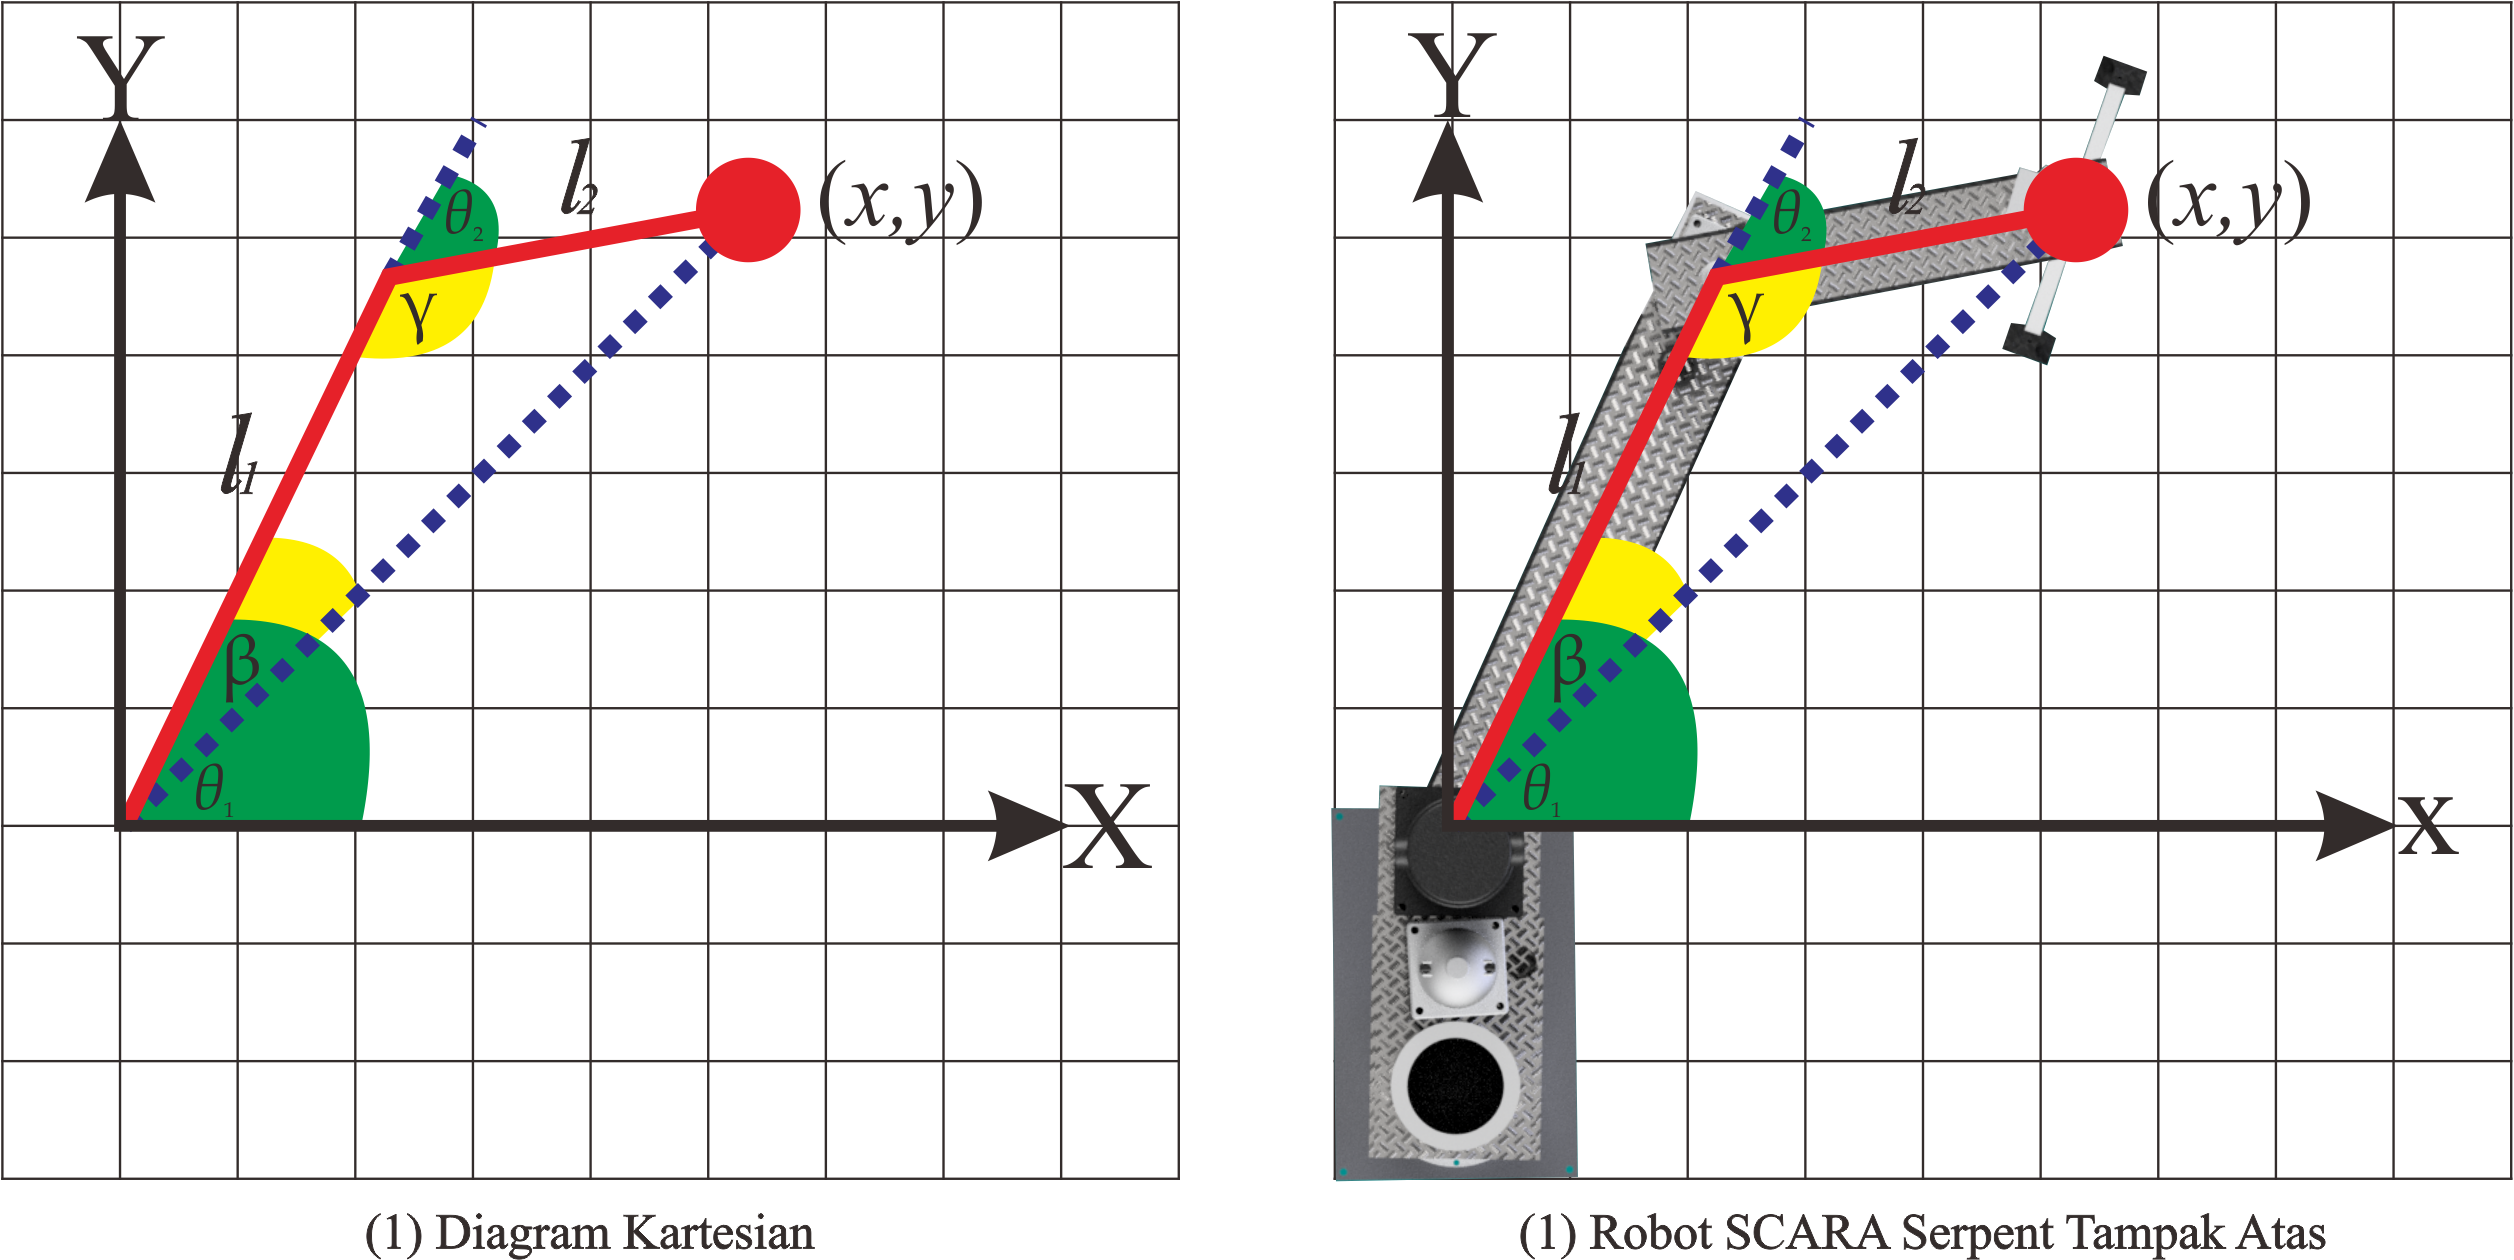
\includegraphics[width=12cm]{gambar/scara_atas.png}
	\caption{Trigonometeri Sisi Atas}
	\label{pic.perskinematikabalik}
\end{figure}
 
 
Pada robot SCARA, sudut dari \textit{joint} yang dicari merupakan \textit{joint} dari \textit{shoulder} dan juga \textit{elbow.} Kedua \textit{joint} tersebut dapat ditemukan dengan melalui persamaan \textit{pythagoras} dan juga hukum \textit{cosinus}. Pada Gambar \ref{pic.perskinematikabalik} terlihat bahwa sudut \textit{shoulder} merupakan besar sudut diantara lengan \textit{shoulder} dan juga sumbu $x$ dan sudut \textit{elbow} merupakan besar sudut antara lengan \textit{elbow} dengan garis bantu dari lengan \textit{shoulder}. Keduanya dapat ditentukan besar nilainya melalui beberapa pesamaan dari \textit{cosinus} dan juga hukum \textit{pyhtagoras}. $l_{1}$ merupakan panjang lengan \textit{shoulder} dan $l_{2}$ merupakan panjang lengan dari \textit{elbow}. Serta $\theta_{1}$ merupakan sudut dari \textit{shoulder} dan $\theta_{2}$ merupakan sudut dari \textit{elbow}\cite{victor}.  

\begin{enumerate}
	\item Dengan menggunakan hukum \textit{cosinus}, didapatkan sebuah Persamaan \ref{cosinus1}
	\begin{equation}
	(x^2+y^2)=l_{1}^2+l_{1}^2-2l_{1}l_{2}cos(180-\theta_{2})
	\label{cosinus1}
	\end{equation}
	\item Pada Persamaan \ref{cosinus1} terdapat $\cos$ yang dapat diubah sesuai dengan prinsip dari hukum \textit{cosinus} menjadi seperti pada Persamaan \ref{cosinus2}
	\begin{equation}
	(x^2+y^2)=l_{1}^2l_{2}^2+2l_{1}l_{2}cos(\theta_{2})
	\label{cosinus2}
	\end{equation}
	\item Inti dari Persamaan \ref{cosinus2} adalah mencari sebuah nilai dari $\theta_{2}$, maka untuk memmudahkannya persamaan menjadi seperti pada Persamaan \ref{cosinus3}
	\begin{equation}
	cos(\theta_{2})=\frac{x^2+y^2-l_{1}^2-l_{2}^2}{2L_{1}l_{2}}
	\label{cosinus3}
	\end{equation}
	\item Nilai dari $\theta_{2}$ dapat dengan mudah diketahui dengan melanjutkan seperti pada Persamaan \ref{cosinus4}
	\begin{equation}
	\theta_{2}=arccos(\frac{x^2+y^2-l_{1}^2-l_{2}^2}{2l_{1}l_{2}})
		\label{cosinus4}
	\end{equation}
	Dengan Persamaan \ref{cosinus4} maka nilai dari $\theta_{2}$ atau sudut dari \textit{elbow} dapat diketahui dengan cara memasukkan nilai posisi $x$, posisi $y$ serta panjang dari \textit{shoulder} dan \textit{elbow} ke dalam persamaan. Nilai posisi $x$ dan posisi $y$ merupakan posisi akhir dari \textit{end-effector}. 
	\item Dalam menentukan sudut lainnya yaitu sudut \textit{shoulder} yang ditandai dengan simbol $\theta_{1}$ menggunakan persamaan \textit{cosinus} yang dituliskan pada Persamaan \ref{cosinus5}
	\begin{equation}
	\frac{sin(\beta)}{l_{2}} = \frac{sin(\gamma)}{\sqrt{x^2+y^2}} ; \alpha=\arctan(\frac{y}{x})
	\label{cosinus5}
	\end{equation}
	\item Pada Persamaan \ref{cosinus5} beberapa nilai dapat diubah sesuai dengan hukum \textit{cosinus} $\sin(\gamma)=\sin(180-\theta_{2})=\sin(\theta_{2})$ dengan mengubah $\sin(\gamma)$ menjadi $\sin(\theta_{2})$ maka akan persamaan menjadi seperti yang ditunjukkan pada Persamaan \ref{cosinus6}
	\begin{equation}
	\beta=\arcsin(\frac{l_{2}\sin(\theta_{2})}{\sqrt{x^2+y^2}})
	\label{cosinus6}
	\end{equation}
	\item Jika dilihat pada gambar \ref{pic.perskinematikabalik} maka besar dari sudut \textit{shoulder} yang ditandakan dengan $\theta_{1}$ yang artinya $\theta_{1}=\beta+\alpha$ maka dapat diselesaikan seperti Persamaan \ref{cosinus7}
	\begin{equation}
	\theta_{1}=\arcsin(\frac{l_{2}\sin(\theta_{2})}{\sqrt{x^2+y^2}}+\arctan(\frac{y}{x})
	\label{cosinus7}
	\end{equation}
	\item  Dengan penyelesaian seperti pada Persamaan \ref{cosinus7} besar sudut dari \textit{shoulder} dapat diketahui dengan memasukkan nilai panjang \textit{elbow}, sudut \textit{elbow} dan juga posisi dari \textit{end-effector}.
\end{enumerate}

Dalam penelitian kinematika robot SCARA ini, segala perhitungan kinematika dilakukan di dalam program Processing IDE. Di dalam Processing IDE terdapat animasi dari bentuk asli robot SCARA. Pada posisi \textit{end-effector} didapat posisi $x$ dan $y$ yang diprogram pada dalam Processing IDE. Dua buah data sudut yang didapat pada perhitungan merupakan sudut \textit{shoulder} dan \textit{elbow} kemudian dikirimkan kepada Arduino Mega 2560 untuk diprores dan diimplemintasikan secara langsung pada robot lengan.

\section{Perancangan Sistem Keseluruhan}
Rancangan sistem keseluruhan merupakan gabungan dari perancangan perangkat keras dan perangkat lunak yang diintegrasikan sesuai dengan diagram blok sistem. Gambar \ref{pic.sistemkeseluruhan} adalah gambaran tentang perancangan sistem secara keseluruhan. Tabel \ref{tbl.sistemkeseluruhan}  menunjukkan keterangan setiap komponen yang ada di dalam sistem keseluruhan \textit{arm manipulator} robot SCARA. 
\begin{figure}[H]
	\centering
	\includegraphics[width=12cm]{gambar/sistem_keseluruhan.png}
	\caption{Sistem Secara Keseluruhan}
	\label{pic.sistemkeseluruhan}
\end{figure}

\begin{table}[H]
	\centering
	\caption{Keterangan Sistem Keseluruhan}
\label{tbl.sistemkeseluruhan}
		\begin{tabular}{|c|l|}
			\hline
			\rowcolor[HTML]{9B9B9B} 
			No & \multicolumn{1}{c|}{\cellcolor[HTML]{9B9B9B}Keterangan} \\ \hline
			1  & Object                                    \\ \hline
			2  & GUI                                              \\ \hline
			3  & Laptop                                        \\ \hline
			4  & \textit{Box} panel                                       \\ \hline
			5  & \textit{Workspace} \\ \hline
			6  & Robot lengan SCARA	                                    \\ \hline
	
		\end{tabular}

\end{table}
Processing IDE merupakan piranti yang digunakan sebagai masukan data. Masukan dari Processing IDE adalah hasil dari perhitungan kinematika maju dan atau kinematika balik yang dimasukkan melalui GUI. Objek berada dalam cakupan \textit{workspace} yang telah ditentukan luasnya yang ditinjau dari cangkupan dari \textit{end-effector}. GUI dari Processing IDE ini diproses menggunakan komputer personal.  

Processing IDE juga menampilan nilai derajat setiap \textit{joint}, koordinat $x$ dan $y$ dari \textit{end-effector}. Koordinat $x$ dan $y$ yang telah didapatkan dari processing IDE diolah dalam perhitungan kinematika balik sehingga dapat ditemukan nilai besar derajat sudut setiap \textit{joint}. Setelah nilai besar derajat sudut setiap \textit{joint} didapatkan, Processing IDE akan mengirimkan nilai tersebut ke Arduino Mega 2560 melewati komunikasi Serial. Arduino Mega 2560 mengirimkan nilai-nilai tersebut sesuai dengan pin motor DC yang tersambung dengan Arduino Mega 2560 melalui \textit{driver} motor H-\textit{Bridge} EMS 30A, kemudian nilai-nilai \textit{joint}  tersebut dikirimkan Arduino Mega 2560 kembali ke Processing IDE melalui koneksi langsung menggunakan kabel USB.  

Arduino Mega 2560 merupakan mikrokotroler yang menggerakkan setiap motor DC sesuai dengan besaran nilai yang telah didapatkan. Robot lengan SCARA akan mencapai koordinat $x$ dan $y$ dari objek, lalu mencengkram objek tersebut menggunakan \textit{gripper}.


\chapter{PENGUJIAN DAN PEMBAHASAN}
Pada bab pengujian dan pembahasan ini, penulis akan melakukan pengujian sistem kendali robot lengan robot SCARA Serpent berdasarkan spesifikasi sistem yang telah dijelaskan pada bab sebelumnya. Tujuan pengujian ini adalah untuk membuktikan apakah sistem yang diimplementasikan telah memenuhi spesifikasi dan rancangan yang sudah direncanakan sebelumnya. Hasil dari pengujian akan dimanfaatkan untuk menyempurnakan kinerja dari sistem dan sekaligus digunakan dalam pengembangan sistem lebih lanjut. 

Metode pengujian menggunakan dua macam metode, yaitu pengujian fungsionalitas dari setiap komponen dan pengujian sistem secara keseluruhan. Pengujian fungsionalitas digunakan untuk membuktikan apakah sistem yang diimplementasikan dapat memenuhi persyaratan dari fungsi operasional yang telah dirancang dan direncanakan sebelumnya. Sedangkan pengujian sistem secara keseluruhan bertujuan untuk memperoleh beberapa parameter yang dapat menunjukkan kemampuan dan keandalan dari sistem secara keseluruhan dalam menjalankan fungsi operasionalnya. Pada sistem robot lengan robot SCARA Serpent dilakukan terlebih dahulu pengujian terhadap fungsional dari beberapa komponen seperti bagian \textit{DC to DC converter}, arah gerakan motor DC, \textit{feedback} potensiometer, fungsi rangkaian \textit{switching} pada \textit{valve pneumatic} dan keakuratan setiap \textit{joint} untuk bergerak sesuai sudut yang diinginkan berdasarkan kinematika balik maupun kinematika maju dengan menggunakan kontrol dari GUI.  Kemudian setelah pengujian fungsional terpenuhi maka dilakukan pengujian sistem secara keseluruhan untuk mengetahui keakuratan dan simulasi dari sistem \textit{arm manipulator} robot SCARA Serpent.

\section{Pengujian Fungsional}
Pengujian fungsional digunakan untuk menguji bagian – bagian dari sistem yang terdiri dari \textit{DC to DC converter}, arah gerakan motor DC, \textit{feedback} potensiometer, fungsi rangkaian \textit{switching} pada \textit{valve pneumatic} dan keakuratan setiap \textit{joint}, pengujian GUI Processing dan pengujian program. 

\subsection{Pengujian DC - to - DC Converter}
Pengujian DC – to – DC \textit{converter} dilakukan untuk mengetahui tegangan masukan pada Arduino Mega 2560, sensor potensiometer, motor DC dan juga sumber tegangan untuk\textit{ valve pneumatic}. Tegangan masukan dari catu daya utama sebesar 24 Volt DC yang nantinya dibagi ke tiga buah nilai tegangan. Tabel \ref{tbl.dctodc} merupakan tegangan keluaran DC – to - DC.

\begin{table}[H]
	\centering
	\caption{Hasil Tegangan Keluaran Dari Tegangan DC-DC Converter}
	\label{tbl.dctodc}
	\begin{tabular}{|c|c|c|c|}
		\hline
		\rowcolor[HTML]{9B9B9B} 
		No & \begin{tabular}[c]{@{}c@{}}Tegangan \\ Masukan (V)\end{tabular} & \begin{tabular}[c]{@{}c@{}}Tegangan Keluaran \\ Buck Converter (12 V)\end{tabular} & \begin{tabular}[c]{@{}c@{}}Tegangan Keluaran \\ Buck Converter (5 V)\end{tabular} \\ \hline
		1  & 12                                                              & 12.1                                                                               & 4.9                                                                               \\ \hline
		2  & 14                                                              & 12.1                                                                               & 4.9                                                                               \\ \hline
		3  & 16                                                              & 12.1                                                                               & 4.9                                                                               \\ \hline
		4  & 18                                                              & 12.1                                                                               & 4.9                                                                               \\ \hline
		5  & 20                                                              & 12.1                                                                               & 4.9                                                                               \\ \hline
	\end{tabular}
\end{table} 

Pada hasil yang ditunjukkan oleh Tabel \ref{tbl.dctodc} terlihat bahwa nilai tegangan telah sesuai dengan yang dibutuhkan. Tegangan 12.1 sudah cukup untuk mengoperasikan motor DC dan tegangan 4.9 sudah dapat untuk mengoperasikan Arduino Mega 2560 dan beberapa sensor. Terlihat bahwa berapapun nilai tegangan masukan, hasil keluarannya tetap. Pada saat mengubah besar tegangan keluaran yang dilakukan oleh Regulator \textit{Buck} LM2596 dilakukan dengan cara memutar potensiometer yang terdapat pada Regulator \textit{Buck}. Diputar searah dengan jarum jam hingga pada teganangan yang diinginkan.
\subsection{Pengujian Motor DC}
Pengujian motor DC dilakukan untuk mengetahui apakah motor DC dalam keaadaan baik atau tidak. Pengujian dilakukan dengan memberikan tegangan kerja pada motor DC yang ada pada \textit{shoulder}, \textit{elbow}, dan juga \textit{end-effector} yang nantinya diukur arus yang dihasilkan pada masing-masing motor DC. Nilai arus yang terukur pada motor DC pasti pada masing-masing motor memiliki besaran yang berbeda. Nilai arus tergantung pada beban yang dimiliki pada masing-masing motor DC dimana semakin besar beban maka samakin besar arus yang akan dihasilkan. Tabel \ref{tbl.motordc} merupakan hasil dari pengujian pada masing-masing motor DC.

\begin{table}[h]
	\centering
	\caption{Hasil Pengujian Motor DC}
	\label{tbl.motordc}
	\begin{tabular}{|c|c|c|c|c|}
		\hline
		\rowcolor[HTML]{9B9B9B} 
		No & \textit{Joint}        & Tegangan(V) & Arus Minimal(A) & Arus Maksimal(A)\\ \hline
		1  & \textit{Shoulder}     & 12.1        &   0,35       & 0,4 \\ \hline
		2  & \textit{Elbow}        & 12.1        &   0,31       & 0,36\\ \hline
		3  & \textit{End-Effector} & 12.1        &   0,6      & 1,2\\ \hline
	\end{tabular}
\end{table}

Pada hasil yang ditunjukkan oleh Tabel \ref{tbl.motordc} menujukkan bahwa setiap motor DC mempunyai nilai arus yang berbeda-beda. Motor DC mengeluarkan arus maksimal saat awal dioperasikan atau pada saat proses \textit{starting. }Motor DC yang terletak pada \textit{end-effcetor} merupakan motor DC yang menghasilkan arus paling besar. Hal ini disebabkan karena motor DC yang terpasang pada \textit{end-effector} dibantu dengan bantuan \textit{belt} untuk menyalurkan putaran pada\textit{ end-effector}. Dengan begitu penggunaan \textit{belt} pada motor DC ini menyebabkan beban yang dikerjakan oleh motor DC pada \textit{end-effector} menjadi lebih besar dari pada motor DC yang lain yang langsung menggerakkan pada masing-masing \textit{joint}. Secara keseluruhan motor DC dapat dioperasikan dan masih dalam keadaan baik.

\subsection{Pengujian \textit{Driver} Motor H – \textit{Bridge}}
Pengujian \textit{driver} motor\textit{ H –} \textit{Bridge} dilakukan untuk mengetahui keberfungsian dari \textit{driver} motor apakah sesuai dengan perancangan atau tidak mulai dari arah putarannya hingga arus yang terukur pada masing-masing \textit{driver} motor. Tabel \ref{tbl.drivermotor1} menunjukkan hasil dari pengujian dari \textit{driver} motor H-\textit{Bridge}. 

\begin{longtable}{|c|l|c|c|l|c|}
	\caption{Hasil Pengujian \textit{Driver} Motor H-\textit{Bridge}}
	\label{tbl.drivermotor1}\\
	\hline
	\rowcolor[HTML]{656565} 
	\cellcolor[HTML]{656565}                     & \multicolumn{1}{c|}{\cellcolor[HTML]{656565}}                        & \multicolumn{2}{c|}{\cellcolor[HTML]{656565}Sinyal Arduino} & \multicolumn{1}{c|}{\cellcolor[HTML]{656565}}                          & \cellcolor[HTML]{656565}                            \\ \cline{3-4}
	\rowcolor[HTML]{656565} 
	\multirow{-2}{*}{\cellcolor[HTML]{656565}No} & \multicolumn{1}{c|}{\multirow{-2}{*}{\cellcolor[HTML]{656565}\textit{Joint}}} & MEN1                         & MEN2                         & \multicolumn{1}{c|}{\multirow{-2}{*}{\cellcolor[HTML]{656565}Kondisi}} & \multirow{-2}{*}{\cellcolor[HTML]{656565}Arus (mA)} \\ \hline
	\endfirsthead
	%
	\endhead
	%
	&                                                                      & HIGH                         & HIGH                         & Tidak berputar                                                         & 0                                                   \\ \cline{3-6} 
	&                                                                      & HIGH                         & LOW                          & Berputar searah putaran jam                                            & 0,37                                                \\ \cline{3-6} 
	&                                                                      & LOW                          & HIGH                         & Berputar berlawanan arah jam                                           & 0,37                                                \\ \cline{3-6} 
	\multirow{-4}{*}{1}                          & \multirow{-4}{*}{\textit{Shoulder}}                                           & LOW                          & LOW                          & Tidak berputar                                                         & 0                                                   \\ \hline
	&                                                                      & HIGH                         & HIGH                         & Tidak berputar                                                         & 0                                                   \\ \cline{3-6} 
	&                                                                      & HIGH                         & LOW                          & Berputar searah putaran jam                                            & 0,33                                                \\ \cline{3-6} 
	&                                                                      & LOW                          & HIGH                         & Berputar berlawanan arah jam                                           & 0,33                                                \\ \cline{3-6} 
	\multirow{-4}{*}{2}                          & \multirow{-4}{*}{\textit{Elbow}}                                              & LOW                          & LOW                          & Tidak berputar                                                         & 0                                                   \\ \hline
	&                                                                      & HIGH                         & HIGH                         & Tidak berputar                                                         & 0                                                   \\ \cline{3-6} 
	&                                                                      & HIGH                         & LOW                          & Berputar searah putaran jam                                            & 0,8                                                 \\ \cline{3-6} 
	&                                                                      & LOW                          & HIGH                         & Berputar berlawanan arah jam                                           & 0,8                                                 \\ \cline{3-6} 
	\multirow{-4}{*}{3}                          & \multirow{-4}{*}{\textit{End-Effector}}                                       & LOW                          & LOW                          & Tidak berputar                                                         & 0                                                   \\ \hline
\end{longtable}
Pada \textit{driver} motor H-\textit{Bridge} EMS 30A sinyal digital HIGH dan LOW dihubungkan pada pin MEN1 dan MEN2. Dari hasil pengujian \textit{driver} motor H-\textit{Bridge} seperti yang ditunjukkan pada Tabel \ref{tbl.drivermotor1} terlihat bahwa ketika sinyal HIGH diberikan pada MEN1 dan LOW diberikan MEN2 maka pergerakan motor akan berputar searah dengan arah jarum jam dan sebaliknya jika diberikan LOW pada MEN1 dan HIGH pada MEN2 maka arah pergerakan motor akan berlawanan arah. Pada Tabel \ref{tbl.drivermotor1}juga terlihat bahwa nilai arus dapat dialirkan pada \textit{driver} motor beragam dari 0,3 Ampere hingga 0,8 Ampere tergangtung pada beban pada masing-masing motor DC. Terlihat bahwa \textit{driver} motor dapat mengoperasikan \textit{driver} motor dengan baik.

\subsection{Pengujian Nilai Analog Potensiometer}
Pengujian nilai analog potensiometer berfungsi untuk mengetahui apakah potensiometer bekerja dengan baik dan nilai yang diberikan dalam keadaan yang normal. Pada potensiometer nilai data yang dikirimkan berupa data analog yang dihasilkan oleh pembagian tegangan yang diatur pada setiap putaran resistornya yang dapat diimplementasikan sebagai posisi sesuai besaran sudut yang dapat dilakukan oleh \textit{joint} yaitu dari 0-360 derajat. Tabel \ref{tbl.potensiometer}.

\begin{table}[H]
	\centering
	\caption{Hasil Pengujian Potensiometer}
	\label{tbl.potensiometer}
	\begin{tabular}{|c|c|c|c|c|c|c|}
		\hline
		\rowcolor[HTML]{9B9B9B} 
		\cellcolor[HTML]{9B9B9B}                            & \multicolumn{2}{c|}{\cellcolor[HTML]{9B9B9B}Joint Shoulder} & \multicolumn{2}{c|}{\cellcolor[HTML]{9B9B9B}Joint Elbow} & \multicolumn{2}{c|}{\cellcolor[HTML]{9B9B9B}End-Effector} \\ \cline{2-7} 
		\rowcolor[HTML]{9B9B9B} 
		\multirow{-2}{*}{\cellcolor[HTML]{9B9B9B}Pengujian} & max                          & min                          & max                         & min                        & max                         & min                         \\ \hline
		Pengujian 1                                         & 761                          & 0                            & 946                         & 1                          & 870                         & 70                          \\ \hline
		Pengujian 2                                         & 762                          & 0                            & 943                         & 1                          & 882                         & 82                          \\ \hline
		Pengujian 3                                         & 762                          & 0                            & 943                         & 1                          & 892                         & 92                          \\ \hline
		Pengujian 4                                         & 761                          & 0                            & 945                         & 1                          & 879                         & 79                          \\ \hline
		Pengujian 5                                         & 762                          & 0                            & 946                         & 1                          & 879                         & 79                          \\ \hline
	\end{tabular}
\end{table} 


Pada hasil pengujian yang ditunjukkan oleh Tabel \ref{tbl.potensiometer} terlihat bahwa pada saat nilai-nilai tertentu potensiometer  mengirimkan nilai data analog yang berubah-ubah. Hal tersebut dipengaruhi oleh pembacaan potensiometer yang belum stabil. Untuk membuat data \textit{analog} yang dikirimkan oleh potensiometer menjadi lebih stabil maka pada program arduino ditambahkan program \textit{moving avarage}. \textit{Moving avarage} berfungi untuk membuat nilai dari hasil data pembacaan pada potensiometer menjadi lebih stabil. 

\textit{Moving avarage} merupakan sebuah formula yang diberikan pada Arduino Mega 2560.  Formula ini menjadikan sebuah pembacaan data yang berubah-ubah pada setiap waktu menjadi lebih stabil. Formula yang ada pada \textit{moving avarage} merupakan hasil rata-rata dari pembacaan data pada sebuah \textit{range} waktu. Beberapa data terbaru akan dijumlahkan dengan data sebelum-sebelumnya kemudian dibagi sesuai dengan jumlah data yang ditambahkan. Hasil data akhir akan mempresentasikan dari pembacaan data yang pada waktu tersebut. Tabel \ref{tbl.potensiometer2} merupakan hasil pengujian nilai data analog potensiometer setelah dilakukan \textit{moving avarage.}

\begin{table}[H]
	\centering
	\caption{Hasil Pengujian Potensiometer Menggunakan Program \textit{Moving Avarage}}
	\label{tbl.potensiometer2}
	\resizebox{9cm}{!}{%
		\begin{tabular}{|c|c|c|c|c|c|c|}
			\hline
			\rowcolor[HTML]{9B9B9B} 
			\cellcolor[HTML]{9B9B9B}                            & \multicolumn{2}{c|}{\cellcolor[HTML]{9B9B9B}Joint Shoulder} & \multicolumn{2}{c|}{\cellcolor[HTML]{9B9B9B}Joint Elbow} & \multicolumn{2}{c|}{\cellcolor[HTML]{9B9B9B}End-Effector} \\ \cline{2-7} 
			\rowcolor[HTML]{9B9B9B} 
			\multirow{-2}{*}{\cellcolor[HTML]{9B9B9B}Pengujian} & max                          & min                          & max                         & min                        & max                         & min                         \\ \hline
			Pengujian 1                                         & 761                          & 0                            & 945                         & 1                          & 886                         & 72                          \\ \hline
			Pengujian 2                                         & 761                          & 0                            & 945                         & 1                          & 887                         & 73                          \\ \hline
			Pengujian 3                                         & 761                          & 0                            & 945                         & 1                          & 886                         & 73                          \\ \hline
			Pengujian 4                                         & 761                          & 0                            & 945                         & 1                          & 886                         & 73                          \\ \hline
			Pengujian 5                                         & 761                          & 0                            & 945                         & 1                          & 886                         & 73                          \\ \hline
		\end{tabular}%
	}
	
\end{table} 


Setelah diberikan sebuah program \textit{moving avarage} terlihat pada Tabel \ref{tbl.potensiometer2} merupakan nilai data yang diterima oleh Arduino Mega 2560 menjadi lebih stabil. Nilai yang stabil akan membantu sebuah sistem dalam melakukan pekerjaannya menjadi lebih baik. Nilai-nilai tersebut nantinya dilakukan proses \textit{mapping} yang menyebabkan nilai minimum dan maksimum yang dihasilkan oleh potensiometer menjadi sesuai dengan posisi dari masing-masing lengan.

\subsection{Pengujian Rangkaian \textit{Switching Valve Pneumatic}}
Pengujian rangkaian \textit{switching} berfungsi untuk mengetahui apakah rangkaian dapat bekerja dengan baik. Fungsi utama dari rangkaian \textit{switching} yang diperuntukkan untuk \textit{valve pneumatic} yaitu sebagai saklar penghubung dan pemutus daya. Rangkaian dapat memutus dan menghubungkan daya dengan \textit{trigger} dari sinyal data yang diberikan kepada \textit{gate} yang berupa sinyal digital \textit{HIGH} dan \textit{LOW} dari Arduino Mega 2560. Pengujian dilakukan dengan mengukur keberhasilan rangkaian sebagai rangkaian \textit{switching}. Tabel \ref{tbl.rangkaiantip} merupakan hasil pengujian dari rangkaian \textit{switching} yang dikontrol oleh TIP31.
\begin{table}[H]
	\centering
	\caption{Hasil Pengujian Rangkaian \textit{Switching Vavle Pnemuatic}}
	\label{tbl.rangkaiantip}
	\begin{tabular}{|c|c|c|c|}
		\hline
		\rowcolor[HTML]{9B9B9B} 
		Sinyal & Tegangan Masuk (V) & Arus (A) & Kondisi             \\ \hline
		HIGH   & 24                 & 0,13     & \textit{Valve} bekerja       \\ \hline
		LOW    & 0                  & 0      & \textit{Valve} tidak bekerja \\ \hline
	\end{tabular}
	
\end{table} 

Pada hasil pengujian yang ditunjukkan pada Tabel \ref{tbl.rangkaiantip} terlihat bahwa rangkaian dapat berfungsi dengan baik dan dapat menghubungkan daya menuju \textit{valve pneumatic}. Terlihat bahwa jika sinyal \textit{HIGH} diberikan pada \textit{gate} TIP31 maka rangkaian \textit{switching} akan menjadi rangkaian tertutup dan daya dapat dialirkan yang berarti \textit{valve pneumatic} menjadi hidup dan siap beroprasi. Sebaliknya, jika pada \textit{gate} TIP31 diberikan sinyal \textit{LOW} maka rangkaian \textit{switching} menjadi rangkaian terbuka dan \textit{valve pneumatic} tidak dapat bekerja.

%\subsection{Pengujian Kinematika Maju}


\subsection{Pengujian Kinematika Balik}
Pengujian kinematika balik pada robot lengan SCARA Serpent dilakukan dengan cara membandingkan posisi koordinat $x$, dan $y$ yang aktual dengan jarak koordinat $x$ dan $y$ yang ada di dalam program Processing IDE. Setiap koordinat dimasukkan ke dalam perhitungan kinematika balik di dalam Processing IDE dan menghasilkan keluaran titik koordinat $x$ dan $y$ pada \textit{end-effector}. Motor DC akan menggerakan lengan \textit{shoulder} dan \textit{elbow} menuju posisi koordinat $x$ dan $y$ sesuai dari yang diperintahkan dalam program.

Pengujian ini dilakukan bertujuan untuk mengetahui \textit{workspace} dari robot lengan SCARA Serpent dan juga mengetahui akurasi dari posisi \textit{end-effector} dengan perhitungan kinematika yang ada. Dalam pengujian ini, pengujian terdiri dari pengujian posisi koordinat posisi \textit{end-effector}, dan juga hasil keluaran sudut pada masing-masing \textit{joint} apakah sesuai dengan posisi \textit{end-effector} yang diberikan. Sudut yang terdiri dari sudut \textit{shoulder} dan sudut \textit{elbow} yang dibandingkan dari pergerakan aslinya dan juga pergerakan pada Processing IDE.  

\subsubsection{Pengujian Koordinat X}

Pengujian koordinat $x$ dilakukan untuk mengetahui batas minimal dan batas maksimal \textit{end-effector} dari \textit{arm manipulator} robot SCARA Serpent relatif terhadap sumbu $x$. Pengujian koordinat $x$ dilakukan dengan cara mengujicobakan setiap titik dari 2 cm sampai dengan total panjang \textit{shoulder} dan \textit{elbow} yaitu 80 cm menggunakan perhitungan kinematika balik. Perhitungan posisi $x$ diujicobakan menggunakan program Processing IDE, sementara untuk pengukuran posisi diukur secara faktual dari posisi \textit{end-effector} dengan membuat sebuah diagram kartesian. Tabel \ref{tbl.x} menunjukkan pengujian koordinat $x$ dan Gambar \ref{pic.koordinatx} menunjukkan grafik dari \textit{sampling} koordinat $x$.

\fontsize{8}{10}\selectfont

\begin{longtable}{|c|c|c|c|c|c|}
	
	\caption{Pengujian Koordinat X}
	\label{tbl.x}\\
	\hline
	
	
	\rowcolor[HTML]{656565} 
	\cellcolor[HTML]{656565}                     & \multicolumn{2}{c|}{\cellcolor[HTML]{656565}X} & \multicolumn{2}{c|}{\cellcolor[HTML]{656565}Y} & \cellcolor[HTML]{656565}                           \\ \cline{2-5}
	\rowcolor[HTML]{656565} 
	\multirow{-2}{*}{\cellcolor[HTML]{656565}No} & Masukan                & Keluran               & Masukan               & Keluaran               & \multirow{-2}{*}{\cellcolor[HTML]{656565}Error(\%)} \\ \hline
	\endfirsthead
	%
	\endhead
	%
	1                                            & 80                     & 75                    & 0                     & 0                      & >5                                               \\ \hline
	2                                            & 78                     & 75                    & 0                     & 0                      & 3,85                                               \\ \hline
	3                                            & 76                     & 75                    & 0                     & 0                      & 1,32                                               \\ \hline
	4                                            & 74                     & 75                    & 0                     & 0                      & 1,35                                               \\ \hline
	5                                            & 72                     & 73                    & 0                     & 0                      & 1,39                                               \\ \hline
	6                                            & 70                     & 71                    & 0                     & 0                      & 1,43                                               \\ \hline
	7                                            & 68                     & 68                    & 0                     & 0                      & 0,00                                               \\ \hline
	8                                            & 66                     & 66                    & 0                     & 0                      & 0,00                                               \\ \hline
	9                                            & 64                     & 64                    & 0                     & 0                      & 0,00                                               \\ \hline
	10                                           & 62                     & 62                    & 0                     & 0                      & 0,00                                               \\ \hline
	11                                           & 60                     & 60                    & 0                     & 0                      & 0,00                                               \\ \hline
	12                                           & 58                     & 56                    & 0                     & 0                      & 3,45                                               \\ \hline
	13                                           & 56                     & 55                    & 0                     & 0                      & 1,79                                               \\ \hline
	14                                           & 54                     & 53                    & 0                     & 0                      & 1,85                                               \\ \hline
	15                                           & 52                     & 51                    & 0                     & 0                      & 1,92                                               \\ \hline
	16                                           & 50                     & 49                    & 0                     & 0                      & 2,00                                               \\ \hline
	17                                           & 48                     & 48                    & 0                     & 0                      & 0,00                                               \\ \hline
	18                                           & 46                     & 46                    & 0                     & 0                      & 0,00                                               \\ \hline
	19                                           & 44                     & 44                    & 0                     & 0                      & 0,00                                               \\ \hline
	20                                           & 42                     & 42                    & 0                     & 0                      & 0,00                                               \\ \hline
	21                                           & 40                     & 40                    & 0                     & 0                      & 0,00                                               \\ \hline
	22                                           & 38                     & 38                    & 0                     & 0                      & 0,00                                               \\ \hline
	23                                           & 36                     & 34                    & 0                     & 0                      & >5                                               \\ \hline
	24                                           & 34                     & 34                    & 0                     & 0                      & 0,00                                               \\ \hline
	25                                           & 32                     & 34                    & 0                     & 0                      & >5                                               \\ \hline
	26                                           & 30                     & 34                    & 0                     & 0                      & >5                                              \\ \hline
	27                                           & 28                     & 34                    & 0                     & 0                      & >5                                              \\ \hline
	28                                           & 26                     & 34                    & 0                     & 0                      & >5                                              \\ \hline
	29                                           & 24                     & 34                    & 0                     & 0                      & >5                                              \\ \hline
	30                                           & 22                     & 34                    & 0                     & 0                      & >5                                              \\ \hline
	31                                           & 20                     & 34                    & 0                     & 0                      & >5                                              \\ \hline
	32                                           & 18                     & 34                    & 0                     & 0                      & >5                                              \\ \hline
	33                                           & 16                     & 34                    & 0                     & 0                      & >5                                            \\ \hline
	34                                           & 14                     & 34                    & 0                     & 0                      & >5                                             \\ \hline
	35                                           & 12                     & 34                    & 0                     & 0                      & >5                                             \\ \hline
	36                                           & 10                     & 34                    & 0                     & 0                      & >5                                             \\ \hline
	37                                           & 8                      & 34                    & 0                     & 0                      & >5                                            \\ \hline
	38                                           & 6                      & 34                    & 0                     & 0                      & >5                                             \\ \hline
	39                                           & 4                      & 34                    & 0                     & 0                      & >5                                             \\ \hline
	40                                           & 2                      & 34                    & 0                     & 0                      & 1600,00                                            \\ \hline	
\end{longtable}

\fontsize{12}{15}\selectfont
\begin{figure}[H]
	\centering
	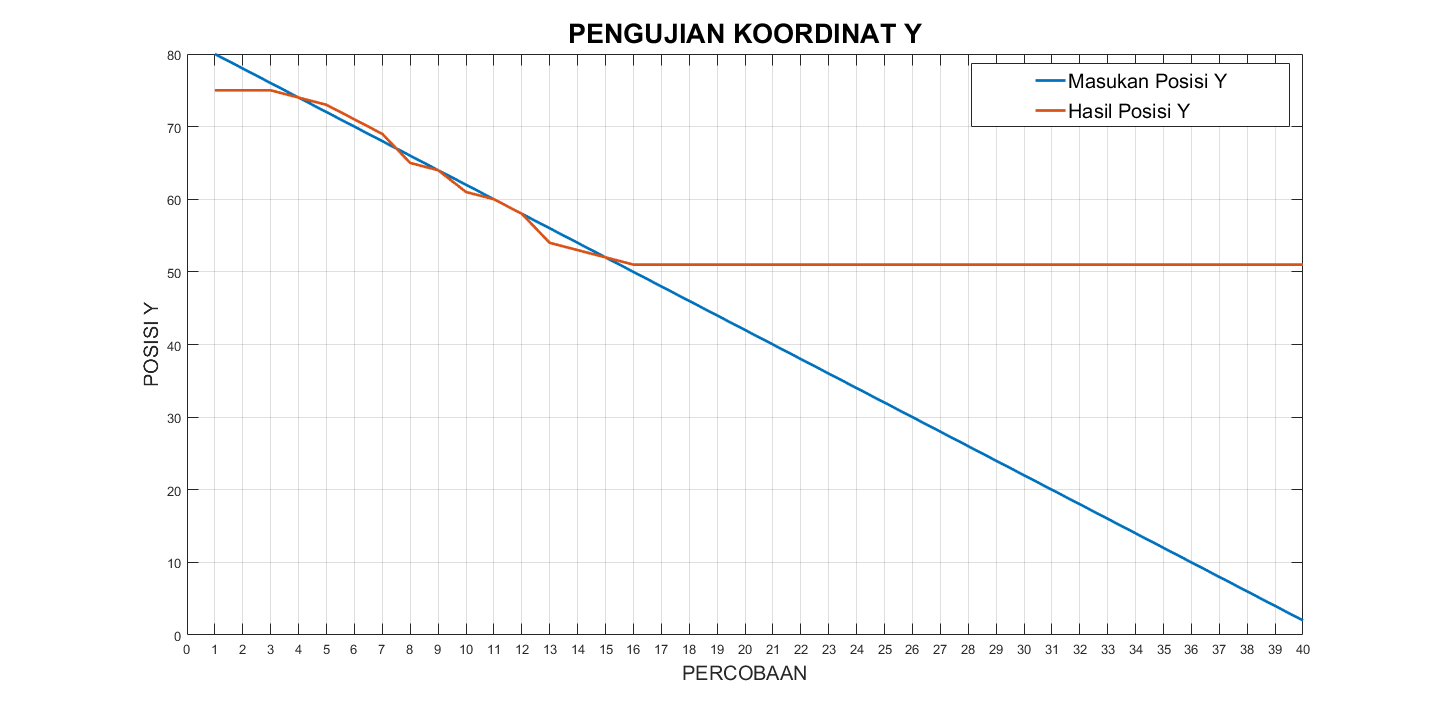
\includegraphics[width=12cm]{gambar/px.png}
	\caption{Grafik Pengujian Koordinat X}
	\label{pic.koordinatx}
\end{figure}

Dari hasil pengujian yang ditampilkan pada Tabel \ref{tbl.x} dan juga Gambar \ref{pic.koordinatx} terlihat bahwa posisi \textit{end-effector} yang dihasilkan pada robot SCARA Serpent dibandingkan dengan data sesuai perhitungan kinematika memiliki sedikit perbedaan pada beberapa data. Perbedaan data ini dapat ditolerasi karena dengan \textit{sampling} koordinat $x$ yang diuji hanya kurang dari lima persen nilai data yang berbeda. Pada hasil yang ditunjukkan diketahui bahwa posisi \textit{end-effector} memiliki batas minimum dan juga maksimum. Batas minimum posisi \textit{end-effector} pada sumbu $x$ yaitu 34 cm dari titik pusat dan batas maksimum posisi \textit{end-effector} pada posisi sumbu $x$ adalah 75 cm yang merupakan panjang dari lengan \textit{shoulder} dan juga lengan \textit{elbow}. Batas ini dapat dilihat bahwa pada Tabel \ref{tbl.x} ketika data masukan diberin nilai kurang dari 34 cm maka posisi \textit{End-Effector} tetap pada posisi 34 cm.


\subsubsection{Pengujian Koordinat Y}
\fontsize{12}{15}\selectfont
Pengujian koordinat $y$ dilakukan untuk mengetahui batas minimal dan batas maksimal \textit{end-effector} dari \textit{arm manipulator} robot SCARA Serpent relatif terhadap sumbu $y$. Pengujian koordinat $y$ dilakukan dengan cara mengujicobakan setiap titik dari 2 cm sampai dengan total panjang \textit{shoulder} dan \textit{elbow} yaitu 80 cm menggunakan perhitungan kinematika balik. Perhitungan posisi $y$ diujicobakan menggunakan program Processing IDE, sementara untuk pengukuran posisi diukur secara faktual dari posisi \textit{end-effector} dengan membuat sebuah diagram kartesius. Tabel \ref{tbl.y} menunjukkan pengujian koordinat $y$ dan Gambar \ref{pic.koordinaty} menunjukkan grafik dari \textit{sampling} koordinat $y$.
% Please add the following required packages to your document preamble:
% \usepackage{multirow}
% \usepackage[table,xcdraw]{xcolor}
% If you use beamer only pass "xcolor=table" option, i.e. \documentclass[xcolor=table]{beamer}
% \usepackage{longtable}
% Note: It may be necessary to compile the document several times to get a multi-page table to line up properly
\fontsize{8}{10}\selectfont
\begin{longtable}{|c|c|c|c|c|c|}
	\caption{Pengujian Koordinat Y}
	\label{tbl.y}\\
	\hline
	\rowcolor[HTML]{9B9B9B} 
	\cellcolor[HTML]{9B9B9B}                     & \multicolumn{2}{c|}{\cellcolor[HTML]{9B9B9B}X} & \multicolumn{2}{c|}{\cellcolor[HTML]{9B9B9B}Y} & \cellcolor[HTML]{9B9B9B}                           \\ \cline{2-5}
	\rowcolor[HTML]{9B9B9B} 
	\multirow{-2}{*}{\cellcolor[HTML]{9B9B9B}No} & Masukan                & Keluran               & Masukan               & Keluaran               & \multirow{-2}{*}{\cellcolor[HTML]{9B9B9B}Error(\%)} \\ \hline
	\endfirsthead
	%
	\endhead
	%
	1                                            & 0                      & 0                     & 80                    & 75                     & >5                                               \\ \hline
	2                                            & 0                      & 0                     & 78                    & 75                     & 3,84                                       \\ \hline
	3                                            & 0                      & 0                     & 76                    & 75                     & 1,31                                       \\ \hline
	4                                            & 0                      & 0                     & 74                    & 74                     & 0                                                  \\ \hline
	5                                            & 0                      & 0                     & 72                    & 73                     & 1,38                                     \\ \hline
	6                                            & 0                      & 0                     & 70                    & 71                     & 1,42                                       \\ \hline
	7                                            & 0                      & 0                     & 68                    & 69                     & 1,47                                       \\ \hline
	8                                            & 0                      & 0                     & 66                    & 65                     & 1,51                                        \\ \hline
	9                                            & 0                      & 0                     & 64                    & 64                     & 0                                                  \\ \hline
	10                                           & 0                      & 0                     & 62                    & 61                     & 1,6                                        \\ \hline
	11                                           & 0                      & 0                     & 60                    & 60                     & 0                                                  \\ \hline
	12                                           & 0                      & 0                     & 58                    & 58                     & 0                                                  \\ \hline
	13                                           & 0                      & 0                     & 56                    & 54                     & 3,57                                      \\ \hline
	14                                           & 0                      & 0                     & 54                    & 53                     & 1,85                                       \\ \hline
	15                                           & 0                      & 0                     & 52                    & 52                     & 0                                                  \\ \hline
	16                                           & 0                      & 0                     & 50                    & 51                     & 2                                                  \\ \hline
	17                                           & 0                      & 0                     & 48                    & 51                     & >5                                               \\ \hline
	18                                           & 0                      & 0                     & 46                    & 51                     & >5                                        \\ \hline
	19                                           & 0                      & 0                     & 44                    & 51                     & >5                                        \\ \hline
	20                                           & 0                      & 0                     & 42                    & 51                     & >5                                        \\ \hline
	21                                           & 0                      & 0                     & 40                    & 51                     & >5                                               \\ \hline
	22                                           & 0                      & 0                     & 38                    & 51                     & >5                                        \\ \hline
	23                                           & 0                      & 0                     & 36                    & 51                     & >5                                        \\ \hline
	24                                           & 0                      & 0                     & 34                    & 51                     & >5                                                 \\ \hline
	25                                           & 0                      & 0                     & 32                    & 51                     & >5                                            \\ \hline
	26                                           & 0                      & 0                     & 30                    & 51                     & >5                                                 \\ \hline
	27                                           & 0                      & 0                     & 28                    & 51                     & >5                                        \\ \hline
	28                                           & 0                      & 0                     & 26                    & 51                     & >5                                        \\ \hline
	29                                           & 0                      & 0                     & 24                    & 51                     & >5                                              \\ \hline
	30                                           & 0                      & 0                     & 22                    & 51                     & >5                                        \\ \hline
	31                                           & 0                      & 0                     & 20                    & 51                     & >5                                                \\ \hline
	32                                           & 0                      & 0                     & 18                    & 51                     & >5                                        \\ \hline
	33                                           & 0                      & 0                     & 16                    & 51                     & >5                                             \\ \hline
	34                                           & 0                      & 0                     & 14                    & 51                     & >5                                        \\ \hline
	35                                           & 0                      & 0                     & 12                    & 51                     & >5                                                \\ \hline
	36                                           & 0                      & 0                     & 10                    & 51                     & >5                                                \\ \hline
	37                                           & 0                      & 0                     & 8                     & 51                     & >5                                              \\ \hline
	38                                           & 0                      & 0                     & 6                     & 51                     & >5                                                \\ \hline
	39                                           & 0                      & 0                     & 4                     & 51                     & >5                                               \\ \hline
	40                                           & 0                      & 0                     & 2                     & 51                     & >5                                              \\ \hline
\end{longtable}
\fontsize{12}{15}\selectfont
\begin{figure}[H]
	\centering
	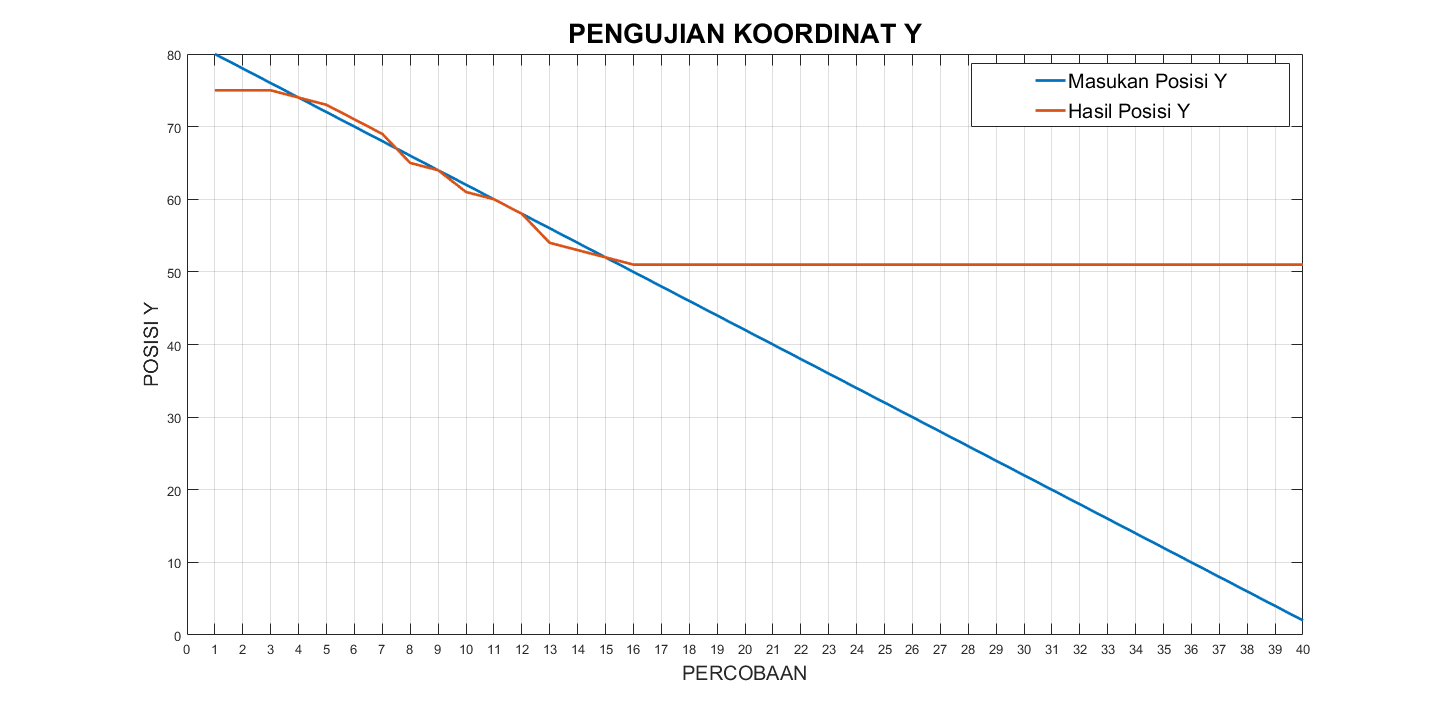
\includegraphics[width=13cm]{gambar/py.png}
	\caption{Grafik Pengujian Koordinat Y}
	\label{pic.koordinaty}
\end{figure}


Dari hasil pengujian yang ditampilkan pada Tabel \ref{tbl.y} dan juga Gambar \ref{pic.koordinaty} terlihat bahwa posisi \textit{end-effector} yang dihasilkan pada robot SCARA Serpent dibandingkan dengan data sesuai perhitungan kinematika memiliki sedikit perbedaan pada beberapa data. Perbedaan data ini dapat ditolerasi karena dengan \textit{sampling} koordinat $y$ yang diuji hanya kurang dari lima persen nilai data yang berbeda. Pada hasil yang ditunjukkan diketahui bahwa posisi \textit{end-effector} memiliki batas minimum dan juga maksimum. Batas minimum posisi \textit{end-effector} pada sumbu $x$ yaitu 51 cm dari titik pusat dan batas maksimum posisi \textit{end-effector} pada posisi sumbu $y$ adalah 75 cm yang merupakan panjang dari lengan \textit{shoulder} dan juga lengan \textit{elbow}.  Batas ini dapat dilihat bahwa pada Tabel \ref{tbl.y} ketika data masukan diberin nilai kurang dari 51 cm maka posisi \textit{end-effector} tetap pada posisi 51 cm.
\subsubsection{\textit{Workspace} Robot Lengan SCARA Serpent }
\textit{Workspace} adalah total volume yang dapat dijangkau oleh \textit{end-effector} robot lengan. Penentuan luas \textit{workspace} ini dibuat dari data pengujian koordinat $x$ dan $y$. Ketinggian maksimum yang dapat dijangkau robot lengan adalah sebesar 25 cm. Jarak minimum yang dapat dijangkau robot lengan pada sumbu $x$ sebesar 31 cm, sementara jarak maksimum yang dapat dijangkau robot lengan sebesar 75 cm. Sedangkan pada sumbu $y$ jarak yang dapat dijangkau robot lengan sebesar 51 cm, sementara jarak maksimum yang dapat dijangkau robot lengan sebesar 75 cm. Titik 0 sampai dengan 31 cm menjadi posisi yang tidak akurat untuk \textit{end-effector} karena jumlah \textit{link} terlalu panjang sedangkan jarak objek terlalu dekat dengan robot lengan, sehingga \textit{end-effector} tidak bisa menjangkau objek pada jarak 0 sampai dengan 31 cm tersebut. Begitupun titik yang lebih dari 75 cm. Jumlah panjang \textit{link} terlalu pendek sedangkan jarak objek terlalu jauh dengan robot lengan, sehingga \textit{end-effector} tidak bida menjangkau objek yang lebih dari 75 cm. Gambar \ref{pic.workpace} merupakan gambaran dari \textit{workspace} yang dihasilkan oleh robot SCARA Serpent.


\begin{figure}[H]
	\centering
	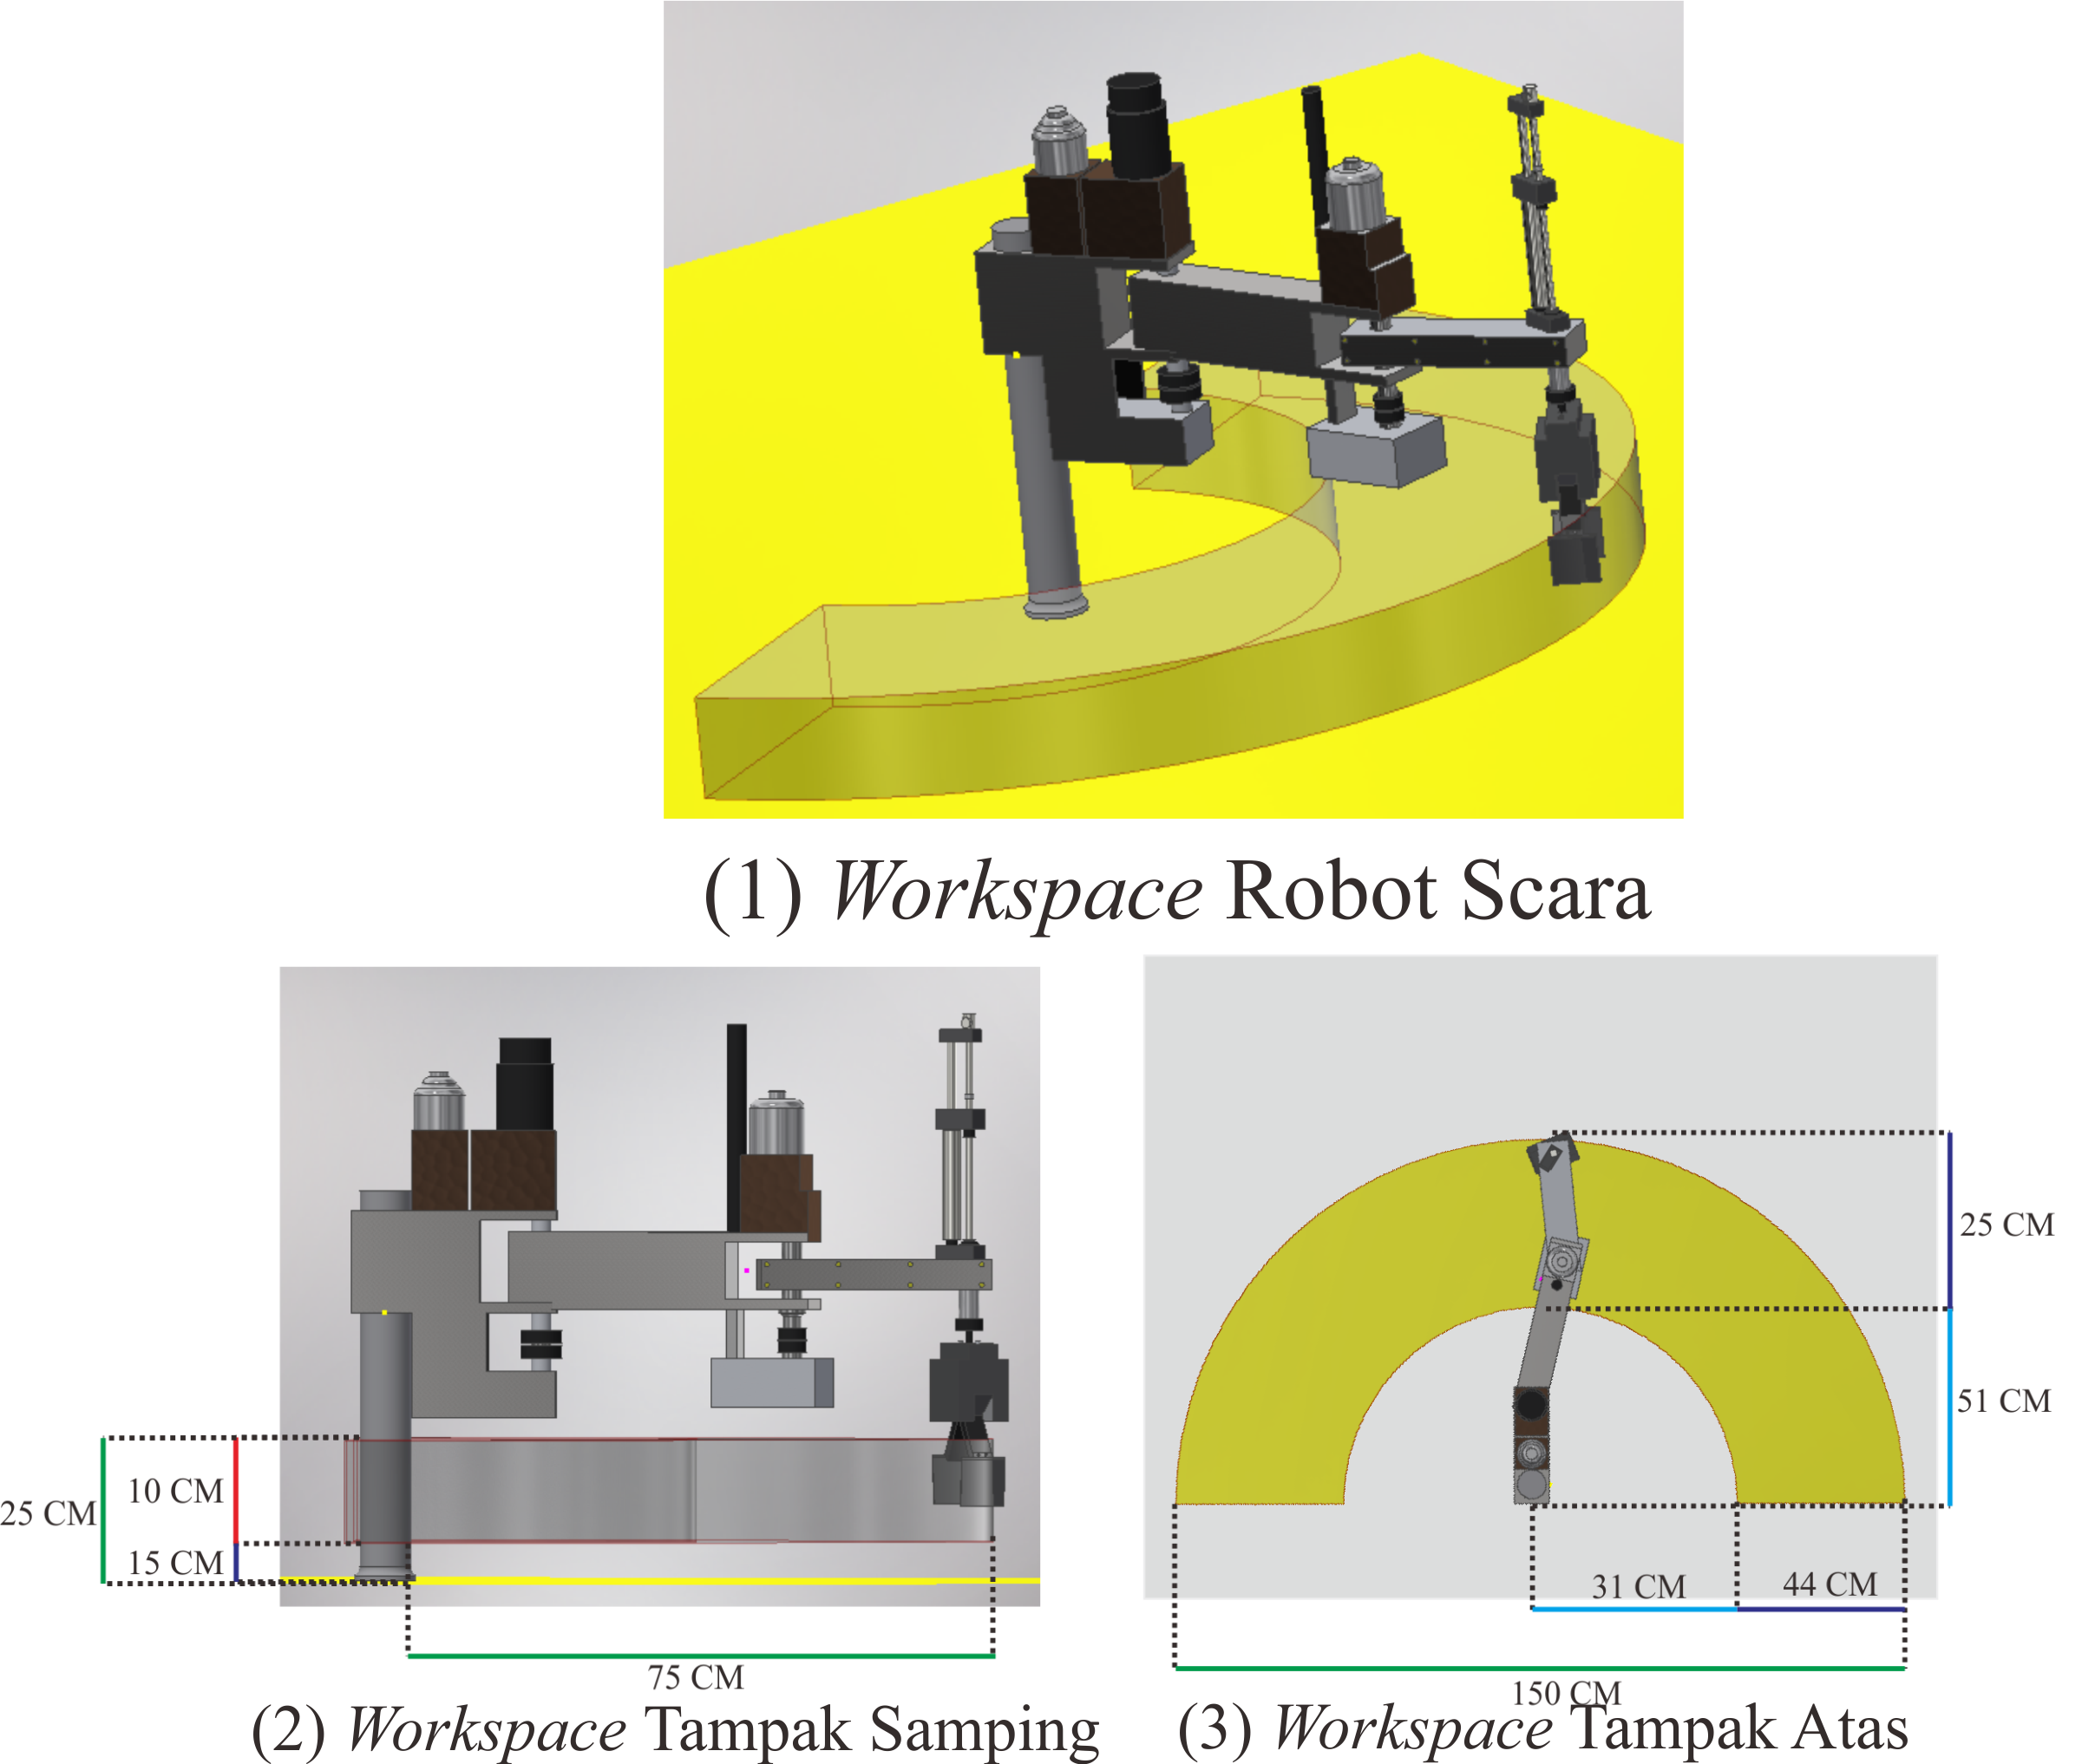
\includegraphics[width=13cm]{gambar/WORKSPACE.png}
	\caption{Workspace Robot SCARA Serpent}
	\label{pic.workpace}
\end{figure}


\subsubsection{Pengujian \textit{Joint Shoulder}}

Pengujian dilakukan dengan cara memberikan sebuah posisi koordinat $x$ dan $y$ dengan nilai yang bervariasi. Nilai tersebut dimasukkan ke dalam sebuah perhitungan kinematika balik yang ada pada program Processing IDE sesuai dengan persamaan pada bab sebelumnya. Hasil yang dihasilkan oleh perhitungan merupakan nilai sudut dari \textit{joint shoulder} dan juga \textit{elbow}. Perhitungan aktual dilakukan dengan cara mengukur sudut pada setiap \textit{joint} menggunakan bantuan busur atau \textit{software} sensor kemiringan yang diunduh pada \textit{smartphone}. Tabel \ref{tbl.shoulder} merupakan hasil pengujian dari \textit{joint shoulder} berdasarkan \textit{sampling} posisi yang diambil. Gambar \ref{pic.jointshoulder} merupakan grafik hubungan dari sudut aktual dan sudut berdasarkan perhitungan kinematika. 
% Please add the following required packages to your document preamble:
% \usepackage[table,xcdraw]{xcolor}
% If you use beamer only pass "xcolor=table" option, i.e. \documentclass[xcolor=table]{beamer}
% \usepackage{longtable}
% Note: It may be necessary to compile the document several times to get a multi-page table to line up properly
\fontsize{8}{10}\selectfont
\begin{longtable}{|c|c|c|c|}
	\caption{Hasil Pengujian \textit{Joint Shoulder}}
	\label{tbl.shoulder}\\
	\hline
	\rowcolor[HTML]{656565} 
	No & Masukan & Keluaran & Error(\%)       \\ \hline
	\endfirsthead
	%
	\endhead
	%
	1  & 0       & 0        & 0           \\ \hline
	2  & 4       & 4        & 0           \\ \hline
	3  & 8       & 8        & 0           \\ \hline
	4  & 12      & 12       & 0           \\ \hline
	5  & 16      & 16       & 0           \\ \hline
	6  & 20      & 20       & 0           \\ \hline
	7  & 24      & 24       & 0           \\ \hline
	8  & 28      & 28       & 0           \\ \hline
	9  & 32      & 33       & 3,12       \\ \hline
	10 & 36      & 35       & 2,77 \\ \hline
	11 & 40      & 40       & 0           \\ \hline
	12 & 44      & 44       & 0           \\ \hline
	13 & 48      & 48       & 0           \\ \hline
	14 & 52      & 52       & 0           \\ \hline
	15 & 56      & 56       & 0           \\ \hline
	16 & 60      & 60       & 0           \\ \hline
	17 & 64      & 64       & 0           \\ \hline
	18 & 68      & 69       & 1,47 \\ \hline
	19 & 72      & 71       & 1,38 \\ \hline
	20 & 76      & 76       & 0           \\ \hline
	21 & 80      & 80       & 0           \\ \hline
	22 & 84      & 84       & 0           \\ \hline
	23 & 88      & 88       & 0           \\ \hline
	24 & 92      & 92       & 0           \\ \hline
	25 & 96      & 96       & 0           \\ \hline
	26 & 100     & 100      & 0           \\ \hline
	27 & 104     & 105      & 0,96 \\ \hline
	28 & 108     & 107      & 0,92 \\ \hline
	29 & 112     & 112      & 0           \\ \hline
	30 & 116     & 116      & 0           \\ \hline
	31 & 120     & 120      & 0           \\ \hline
	32 & 124     & 123      & 0,80 \\ \hline
	33 & 128     & 128      & 0           \\ \hline
	34 & 132     & 132      & 0           \\ \hline
	35 & 136     & 136      & 0           \\ \hline
	36 & 140     & 139      & 0,71 \\ \hline
	37 & 144     & 144      & 0           \\ \hline
	38 & 148     & 148      & 0           \\ \hline
	39 & 152     & 152      & 0           \\ \hline
	40 & 156     & 155      & 0,64 \\ \hline
	41 & 160     & 161      & 0,62       \\ \hline
	42 & 164     & 164      & 0           \\ \hline
	43 & 168     & 168      & 0           \\ \hline
	44 & 172     & 172      & 0           \\ \hline
	45 & 176     & 175      & 0,56 \\ \hline
	46 & 180     & 180      & 0           \\ \hline
\end{longtable}
\fontsize{12}{15}\selectfont
\begin{figure}[H]
	\centering
	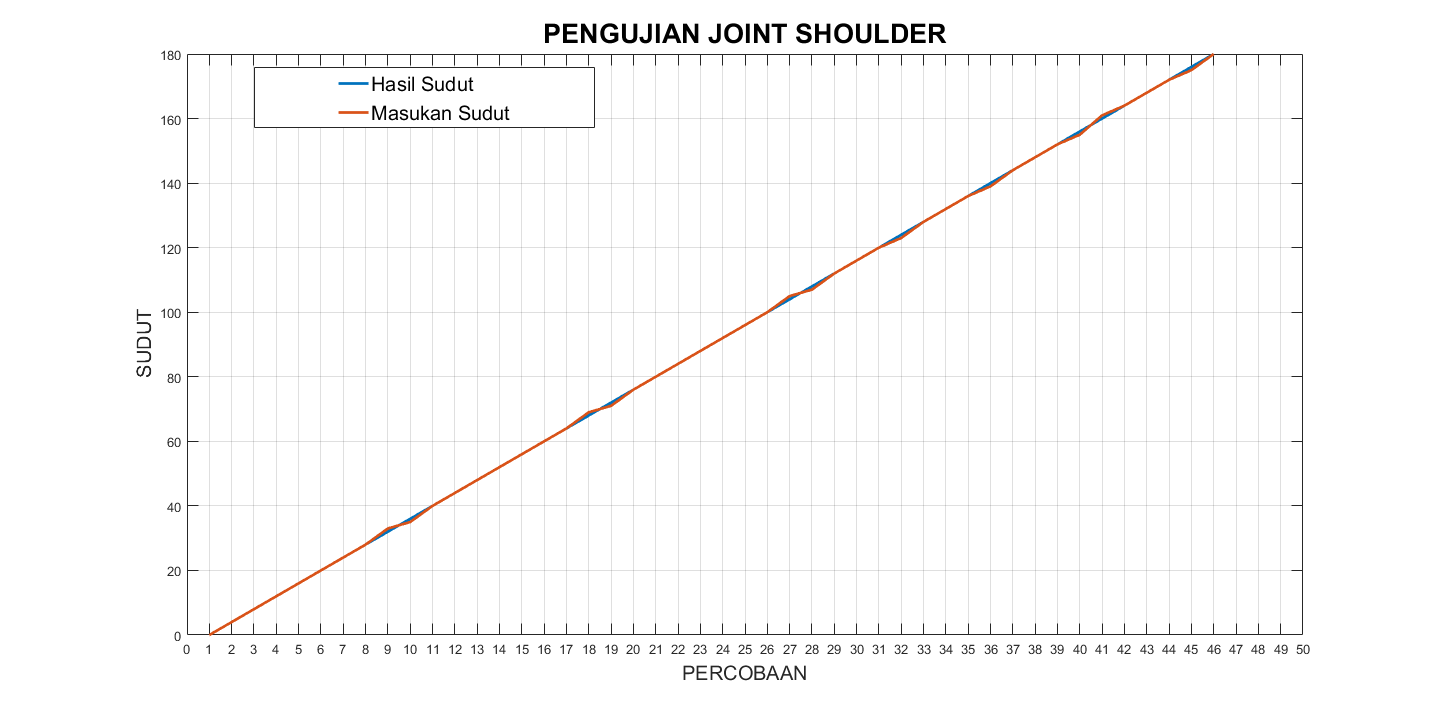
\includegraphics[width=13cm]{gambar/ps.png}
	\caption{Grafik Pengujian \textit{Joint Shoulder}}
	\label{pic.jointshoulder}
\end{figure}

Pada hasil yang ditunjukkan oleh Tabel \ref{tbl.shoulder} dan Gambar \ref{pic.jointshoulder} terlihat bahwa secara keseleuruhan nilai sudut yang dihasilkan oleh aktual pada robot SCARA Serpent dibandingkan dengan perhitungan kinematika oleh Processing IDE tidak begitu terdapat perbedaan. Terlihat bahwa nilai \textit{error}
memiliki nilai minimum 0 persen dan nilai maksimum 2,77 persen. Persentase \textit{error} didapat dari data yang tidak sesuai dibagi oleh keleluruhan data yang diuji coba. Dapat dikatakan bahwa pengujian sudut \textit{joint shoulder} cukup baik.

\subsubsection{Pengujian \textit{Joint Elbow}}

Pengujian \textit{joint elbow} dilakukan dengan membandingkan nilai sudut yang dihasilkan oleh perhitungan kinematika yang ada pada program Processing IDE dengan sudut yang dihasilkan dalam aktual robot SCARA Serpent. Pengujian dilakukan dengan cara memberikan sebuah posisi koordinat $x$ dan $y$ dengan nilai yang bervariasi. Nilai tersebut dimasukkan ke dalam sebuah perhitungan kinematika balik yang ada pada program Processing IDE. Hasil yang dihasilkan oleh perhitungan merupakan nilai sudut dari \textit{joint shoulder} dan juga \textit{elbow}. Perhitungan aktual dilakukan dengan cara mengukur sudut pada setiap \textit{joint} menggunakan bantuan busur atau \textit{software} sensor kemiringan yang diunduh pada \textit{smartphone}. Tabel \ref{tbl.elbow} merupakan hasil pengujian dari \textit{joint elbow} berdasarkan \textit{sampling} posisi yang diambil. Gambar \ref{pic.jointelbow} merupakan grafik hubungan dari sudut aktual dan sudut berdasarkan perhitungan kinematika. 
% Please add the following required packages to your document preamble:
% \usepackage[table,xcdraw]{xcolor}
% If you use beamer only pass "xcolor=table" option, i.e. \documentclass[xcolor=table]{beamer}
% \usepackage{longtable}
% Note: It may be necessary to compile the document several times to get a multi-page table to line up properly
\fontsize{8}{10}\selectfont
\begin{longtable}{|c|c|c|c|}
	\caption{Hasil Pengujian \textit{Joint Elbow}}
	\label{tbl.elbow}\\
	\hline
	\rowcolor[HTML]{656565} 
	No & Masukan & Keluaran & Error(\%)       \\ \hline
	\endfirsthead
	%
	\endhead
	%
	1  & 0       & 1        & 0           \\ \hline
	2  & 4       & 4        & 0           \\ \hline
	3  & 8       & 9        & >5      \\ \hline
	4  & 12      & 13       & >5  \\ \hline
	5  & 16      & 17       & >5         \\ \hline
	6  & 20      & 21       & 5           \\ \hline
	7  & 24      & 25       & 4,16 \\ \hline
	8  & 28      & 29       & 3,57 \\ \hline
	9  & 32      & 32       & 0           \\ \hline
	10 & 36      & 36       & 0           \\ \hline
	11 & 40      & 41       & 2,5         \\ \hline
	12 & 44      & 45       & 2,27 \\ \hline
	13 & 48      & 49       & 2,08 \\ \hline
	14 & 52      & 53       & 1,92 \\ \hline
	15 & 56      & 57       & 1,78 \\ \hline
	16 & 60      & 61       & 1,66 \\ \hline
	17 & 64      & 64       & 0           \\ \hline
	18 & 68      & 67       & 1,47 \\ \hline
	19 & 72      & 72       & 0           \\ \hline
	20 & 76      & 76       & 0           \\ \hline
	21 & 80      & 80       & 0           \\ \hline
	22 & 84      & 84       & 0           \\ \hline
	23 & 88      & 88       & 0           \\ \hline
	24 & 92      & 92       & 0           \\ \hline
	25 & 96      & 96       & 0           \\ \hline
	26 & 100     & 100      & 0           \\ \hline
	27 & 104     & 104      & 0           \\ \hline
	28 & 108     & 108      & 0           \\ \hline
	29 & 112     & 111      & 0,89 \\ \hline
	30 & 116     & 115      & 0,86 \\ \hline
	31 & 120     & 119      & 0,83 \\ \hline
	32 & 124     & 123      & 0,80 \\ \hline
	33 & 128     & 128      & 0           \\ \hline
	34 & 132     & 132      & 0           \\ \hline
	35 & 136     & 136      & 0           \\ \hline
	36 & 140     & 140      & 0           \\ \hline
	37 & 144     & 144      & 0           \\ \hline
	38 & 148     & 148      & 0           \\ \hline
	39 & 152     & 152      & 0           \\ \hline
	40 & 156     & 156      & 0           \\ \hline
	41 & 160     & 160      & 0           \\ \hline
	42 & 164     & 164      & 0           \\ \hline
	43 & 168     & 168      & 0           \\ \hline
	44 & 172     & 172      & 0           \\ \hline
	45 & 176     & 176      & 0           \\ \hline
	46 & 180     & 180      & 0           \\ \hline
\end{longtable}
\fontsize{12}{15}\selectfont
\begin{figure}[H]
	\centering
	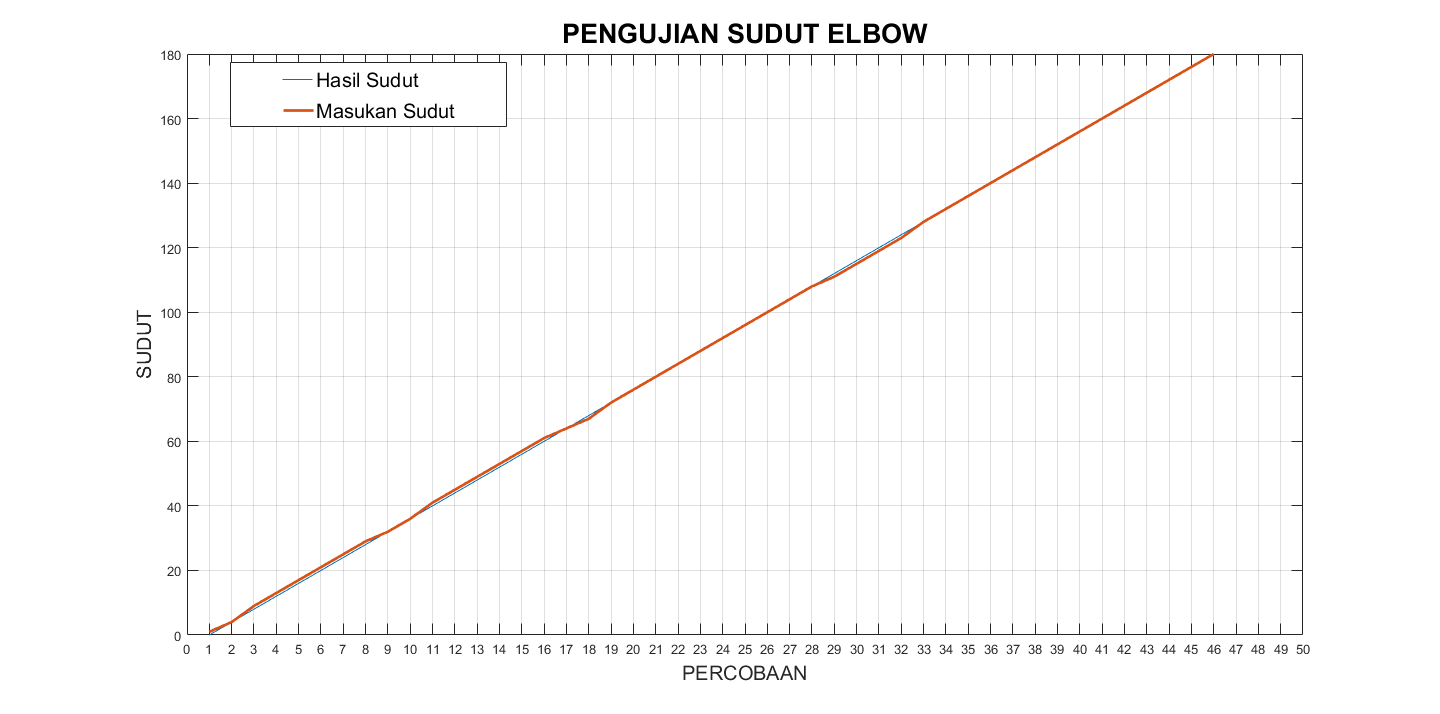
\includegraphics[width=12cm]{gambar/pe.png}
	\caption{Grafik Pengujian \textit{Joint Elbow}}
	\label{pic.jointelbow}
\end{figure}

Pada hasil yang ditunjukkan oleh Tabel \ref{tbl.elbow} dan Gambar \ref{pic.jointelbow} terlihat bahwa secara keseleuruhan nilai sudut yang dihasilkan oleh aktual pada robot SCARA Serpent dibandingkan dengan perhitungan kinematika oleh Processing IDE tidak begitu terdapat perbedaan. Terlihat bahwa nilai \textit{error}
memiliki nilai minimum 0 persen dan nilai maksimum lebih dari 5 persen. Persentase \textit{error} didapat dari data yang tidak sesuai dibagi oleh keleluruhan data yang diuji coba. 


\section{Pengujian Keseluruhan}
Setelah semua komponen sistem yang diuji dapat bekerja dengan baik, pengujian selanjutnya adalah pengujian sistem secara keseluruhan dengan beberapa parameter uji yang diberikan. Parameter uji tersebut diantaranya adalah pengujian akurasi robot lengan, dan simulasi robot lengan. 

\subsection{Pengujian Akurasi Robot Lengan}

Pada pengujian akurasi robot lengan dilakukan pengujian dengan memberikan posisi koordinat $x$ dan $y$ dan melihat kembali posisi $x$ dan $y$ secara aktual, melihat besar sudut pada masing-masing \textit{joint} dengan perbandingan perhitungan kinematika. Pengujian akurasi robot lengan ini akan menghasilkan sebuah hasil secara luas dan dapat ditarik untuk sebuah kesimpulan yang menentukan robot SCARA Serpent dapat bekerja baik atau buruk secara keseluruhan. Tabel \ref{tbl.akurasikeseluruhan} merupakan hasil dari pengujian akurasi robot lengan secara keseluruhan. Gambar \ref{pic.akurasikeseluruhan} merupakan grafik dari hasil pengujian akurasi robot lengan secara keseluruhan.
% Please add the following required packages to your document preamble:
% \usepackage{multirow}
% \usepackage{graphicx}
% \usepackage[table,xcdraw]{xcolor}
% If you use beamer only pass "xcolor=table" option, i.e. \documentclass[xcolor=table]{beamer}
\begin{table}[H]
	\caption{}
	\label{tbl.akurasikeseluruhan}
	\resizebox{\textwidth}{!}{%
		\begin{tabular}{|
				>{\columncolor[HTML]{FFCCC9}}c |
				>{\columncolor[HTML]{FFCCC9}}c |
				>{\columncolor[HTML]{FFCCC9}}c |
				>{\columncolor[HTML]{FFCCC9}}c |
				>{\columncolor[HTML]{FFCCC9}}c |
				>{\columncolor[HTML]{FFFC9E}}c |
				>{\columncolor[HTML]{FFFC9E}}c |
				>{\columncolor[HTML]{FFFC9E}}c |
				>{\columncolor[HTML]{FFCCC9}}c |
				>{\columncolor[HTML]{FFCCC9}}c |
				>{\columncolor[HTML]{FFCCC9}}c |
				>{\columncolor[HTML]{FFFC9E}}c |}
			\hline
			\multicolumn{5}{|c|}{\cellcolor[HTML]{9B9B9B}Posisi (x,y)} & \multicolumn{3}{c|}{\cellcolor[HTML]{9B9B9B}Shoulder} & \multicolumn{3}{c|}{\cellcolor[HTML]{9B9B9B}Elbow} & \cellcolor[HTML]{9B9B9B} \\ \cline{1-11}
			\multicolumn{2}{|c|}{\cellcolor[HTML]{9B9B9B}Input} & \multicolumn{2}{c|}{\cellcolor[HTML]{9B9B9B}Output} & \cellcolor[HTML]{9B9B9B} & \cellcolor[HTML]{9B9B9B} & \cellcolor[HTML]{9B9B9B} & \cellcolor[HTML]{9B9B9B} & \cellcolor[HTML]{9B9B9B} & \cellcolor[HTML]{9B9B9B} & \cellcolor[HTML]{9B9B9B} & \cellcolor[HTML]{9B9B9B} \\ \cline{1-4}
			\cellcolor[HTML]{9B9B9B}x & \cellcolor[HTML]{9B9B9B}y & \cellcolor[HTML]{9B9B9B}x & \cellcolor[HTML]{9B9B9B}y & \multirow{-2}{*}{\cellcolor[HTML]{9B9B9B}Error(\%)} & \multirow{-2}{*}{\cellcolor[HTML]{9B9B9B}Hasil} & \multirow{-2}{*}{\cellcolor[HTML]{9B9B9B}Terukur} & \multirow{-2}{*}{\cellcolor[HTML]{9B9B9B}Error(\%)} & \multirow{-2}{*}{\cellcolor[HTML]{9B9B9B}Hasil} & \multirow{-2}{*}{\cellcolor[HTML]{9B9B9B}Terukur} & \multirow{-2}{*}{\cellcolor[HTML]{9B9B9B}Error(\%)} & \multirow{-3}{*}{\cellcolor[HTML]{9B9B9B}Error Total(\%)} \\ \hline
			0 & 76 & 0 & 75 & Error & 90 & 90,0 & 0,00 & 0 & 0 & Error & Error \\ \hline
			2 & 74 & 2 & 74 & 0,00 & 96 & 95,0 & 0,73 & 16,59 & 16 & 3,56 & 1,43 \\ \hline
			4 & 72 & 4 & 72 & 0,00 & 98,82 & 99,0 & 0,18 & 27,79 & 26 & 6,44 & 2,21 \\ \hline
			6 & 70 & 4 & 70 & 16,67 & 102,66 & 102,0 & 0,64 & 39,5 & 40 & 1,27 & 6,19 \\ \hline
			8 & 68 & 6 & 67 & 13,24 & 104,31 & 103,0 & 1,26 & 48,04 & 48 & 0,08 & 4,86 \\ \hline
			10 & 66 & 9 & 66 & 5,00 & 104,18 & 103,0 & 1,13 & 52,36 & 52 & 0,69 & 2,27 \\ \hline
			12 & 64 & 10 & 64 & 8,33 & 105,2 & 104,0 & 1,14 & 58,63 & 58 & 1,07 & 3,52 \\ \hline
			14 & 62 & 12 & 62 & 7,14 & 105,22 & 104,0 & 1,16 & 64,13 & 64 & 0,20 & 2,84 \\ \hline
			16 & 60 & 14 & 60 & 6,25 & 103,95 & 104,0 & 0,05 & 66,68 & 66 & 1,02 & 2,44 \\ \hline
			18 & 58 & 15 & 59 & 7,47 & 104,08 & 103,0 & 1,04 & 71,58 & 71 & 0,81 & 3,11 \\ \hline
			20 & 56 & 18 & 58 & 3,21 & 102,32 & 102,0 & 0,31 & 73,39 & 73 & 0,53 & 1,35 \\ \hline
			22 & 54 & 20 & 55 & 3,62 & 101,01 & 100,0 & 1,00 & 76,85 & 76 & 1,11 & 1,91 \\ \hline
			24 & 52 & 21 & 54 & 4,33 & 100,03 & 100,0 & 0,03 & 80,18 & 81 & 1,02 & 1,79 \\ \hline
			26 & 50 & 24 & 52 & 1,85 & 97,83 & 97,0 & 0,85 & 81,33 & 81 & 0,41 & 1,03 \\ \hline
			28 & 48 & 26 & 50 & 1,49 & 95,48 & 95,0 & 0,50 & 83,2 & 82 & 1,44 & 1,14 \\ \hline
			30 & 46 & 28 & 48 & 1,16 & 94,01 & 94,0 & 0,01 & 85,9 & 83 & 3,38 & 1,52 \\ \hline
			32 & 44 & 30 & 47 & 0,28 & 91,07 & 92,0 & 1,02 & 85,71 & 84 & 2,00 & 1,10 \\ \hline
			34 & 42 & 32 & 44 & 0,56 & 88,07 & 89,0 & 1,06 & 86,65 & 86 & 0,75 & 0,79 \\ \hline
			36 & 40 & 34 & 43 & 0,97 & 86,01 & 87,0 & 1,15 & 87,02 & 87 & 0,02 & 0,72 \\ \hline
			38 & 38 & 36 & 42 & 2,63 & 82,83 & 84,0 & 1,41 & 87,41 & 87 & 0,47 & 1,50 \\ \hline
			40 & 36 & 39 & 40 & 4,31 & 79,33 & 80,0 & 0,84 & 87,02 & 87 & 0,02 & 1,72 \\ \hline
			42 & 34 & 40 & 36 & 0,56 & 76,78 & 76,0 & 1,02 & 87,8 & 87 & 0,91 & 0,83 \\ \hline
			44 & 32 & 43 & 36 & 5,11 & 73,23 & 73,0 & 0,31 & 85,71 & 86 & 0,34 & 1,92 \\ \hline
			46 & 30 & 44 & 34 & 4,49 & 70,45 & 72,0 & 2,20 & 85,9 & 86 & 0,12 & 2,27 \\ \hline
			48 & 28 & 47 & 33 & 7,89 & 66,8 & 66,0 & 1,20 & 83,2 & 84 & 0,96 & 3,35 \\ \hline
			50 & 26 & 49 & 31 & 8,62 & 62,92 & 62,0 & 1,46 & 81,33 & 83 & 2,05 & 4,04 \\ \hline
			52 & 24 & 52 & 28 & 8,33 & 58,87 & 58,0 & 1,48 & 78,65 & 78 & 0,83 & 3,55 \\ \hline
			54 & 22 & 53 & 26 & 8,16 & 56,09 & 55,0 & 1,94 & 76,85 & 77 & 0,20 & 3,43 \\ \hline
			56 & 20 & 56 & 25 & 12,50 & 51,9 & 51,0 & 1,73 & 73,39 & 75 & 2,19 & 5,48 \\ \hline
			58 & 18 & 58 & 23 & 13,89 & 49,07 & 49,0 & 0,14 & 70,93 & 71 & 0,10 & 4,71 \\ \hline
			60 & 16 & 60 & 21 & 15,63 & 44,62 & 44,0 & 1,39 & 66,68 & 65 & 2,52 & 6,51 \\ \hline
			62 & 14 & 62 & 18 & 14,29 & 40,2 & 40,0 & 0,50 & 62,12 & 64 & 3,03 & 5,94 \\ \hline
			64 & 12 & 64 & 16 & 16,67 & 36,92 & 37,0 & 0,22 & 58,21 & 58 & 0,36 & 5,75 \\ \hline
			66 & 10 & 66 & 14 & 20,00 & 32,11 & 33,0 & 2,77 & 52,36 & 53 & 1,22 & 8,00 \\ \hline
			68 & 8 & 68 & 12 & 25,00 & 28,23 & 29,0 & 2,73 & 48,04 & 48 & 0,08 & 9,27 \\ \hline
			70 & 6 & 70 & 10 & 33,33 & 22,91 & 24,0 & 4,76 & 39,17 & 40 & 2,12 & 13,40 \\ \hline
			72 & 4 & 73 & 8 & 50,69 & 15,91 & 18,0 & 13,14 & 27,79 & 28 & 0,76 & 21,53 \\ \hline
			74 & 2 & 74 & 5 & 75,00 & 9,08 & 12,0 & 32,16 & 16,59 & 17 & 2,47 & 36,54 \\ \hline
			76 & 0 & 75 & 2 & Error & 0 & 2,0 & Error & 0 & 2 & Error & Error \\ \hline
			\multicolumn{4}{|c|}{\cellcolor[HTML]{FFCCC9}TOTAL} & 408,67 & \multicolumn{2}{c|}{\cellcolor[HTML]{FFFC9E}TOTAL} & 84,67 & \multicolumn{2}{c|}{\cellcolor[HTML]{FFCCC9}TOTAL} & 46,54 & 179,96 \\ \hline
			\multicolumn{4}{|c|}{\cellcolor[HTML]{FFCCC9}RATA-RATA} & 10,48 & \multicolumn{2}{c|}{\cellcolor[HTML]{FFFC9E}RATA-RATA} & 2,17 & \multicolumn{2}{c|}{\cellcolor[HTML]{FFCCC9}RATA-RATA} & 1,19 & 4,61 \\ \hline
		\end{tabular}%
	}
\end{table}

\fontsize{12}{15}\selectfont
\begin{table}[H]
	\centering
	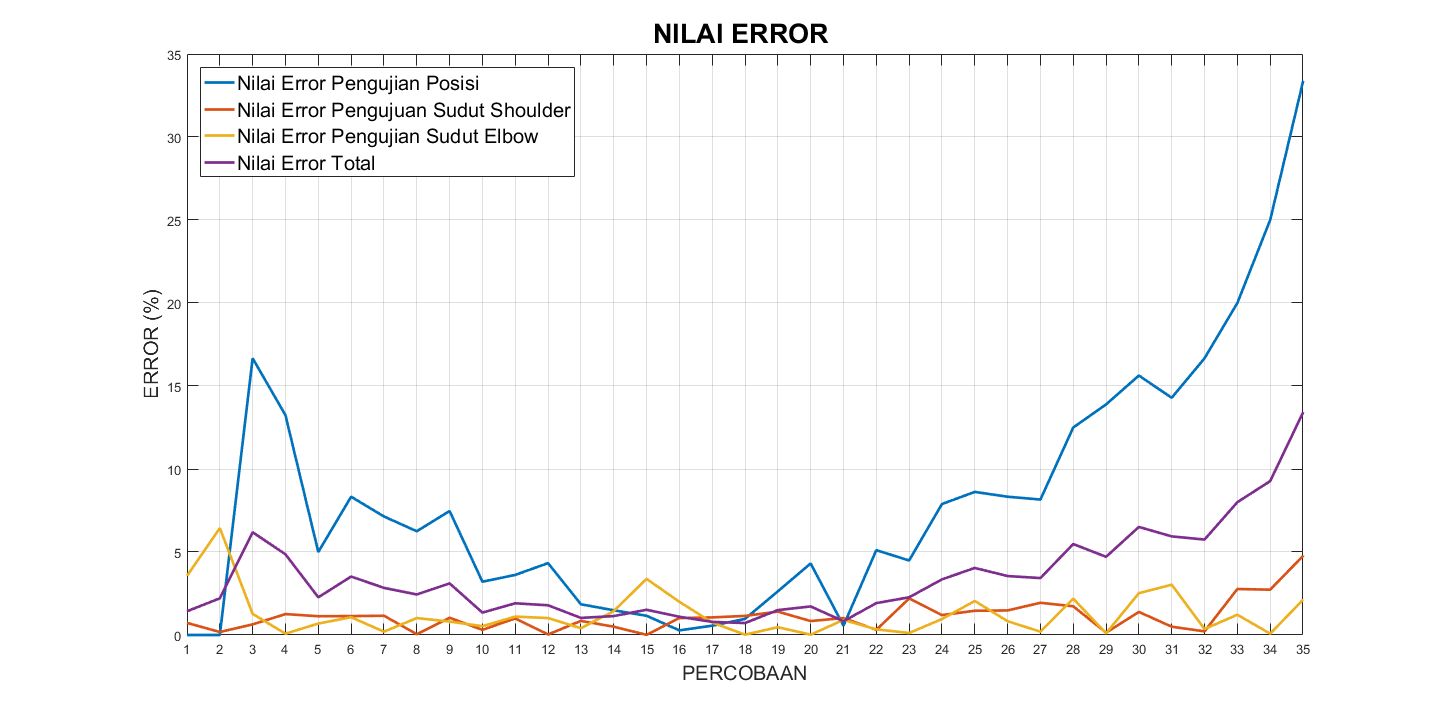
\includegraphics[width=13cm]{gambar/ne.png}
	\caption{Grafik Pengujian Akurasi Robot Secara Keseluruhan}
	\label{pic.akurasikeseluruhan}
\end{table}


Pada hasil pengujian yang ditunjukkan pada Tabel \ref{tbl.akurasikeseluruhan} dan Gambar \ref{pic.akurasikeseluruhan} terlihat bahwa pengujian mendapat beberapa data yang beragam. Terlihat bahwa nilai kesalahan paling banyak terdapat pada bagian posisi koordinat $x$ dan $y$ dan kesalahan paling sedikit pada bagian sudut \textit{shoulder}. Sedangkan untuk sistem keseluruhan kesalahan total pada akurasi robot memiliki nilai 4,61 persen. Nilai sebesar ini merupakan nilai yang cukup baik bagi sebuah sistem. Dengan nilai tersebut maka sistem kinematika robot SCARA Serpent ini dapat dikatakan baik. 


\section{Pengujian Kendali Proposional}
Tujuan dari kendali PID pada sistem ini membuat pergerakan robot mampu menuju sebuah sudut yang diinginkan dengan tingkat \textit{error} paling minimum dengan waktu yang singkat. Sudut pada robot lengan merupakan sudut yang terletak pada \textit{joint shoulder, elbow} dan \textit{end-effector}. Semakin kecil nilai \textit{error} yang dihasilkan dari pengujian kendali PID maka semakin baik pergerakan dari robot lengan. Pengujian PID dilakukan dengan cara memberikan nilai Kp, Ki, dan Kd secara bervariasi dengan melihat respon yang dihasilkan oleh robot SCARA Serpent. Gambar \ref{pic.kendali} merupakan data pengujian dari robot lengan dengan variasi nilai kendali PID yang menghasilkan respon yang berbeda-beda.


\begin{figure}[H]
	\centering
	\includegraphics[width=\textwidth,height=\textheight,keepaspectratio]{gambar/kendali1.png}
\end{figure}

\begin{figure}[H]
	\centering
		\includegraphics[width=\textwidth,height=\textheight,keepaspectratio]{gambar/kendali2.png}
\end{figure}

\begin{figure}[H]
	\centering
		\includegraphics[width=\textwidth,height=\textheight,keepaspectratio]{gambar/kendali3.png}
	\caption{Data Kendali Posisi}
	\label{pic.kendali}
\end{figure}

Dari beberapa nilai Kp, Ki, dan Kd yang coba diberikan kedalam robot lengan SCARA Serpent, terlihat bahwa respon yang didapat beraneka ragam. Respon terbaik ditandai dengan respon yang dapat mencapai \textit{set point} dengan cepat dan dan tepat serta tidak berubah-ubah. Dari beberapa pengujian kendali PID seperti yang ditunjukkan pada Gambar \ref{pic.kendali} terlihat bahwa respon dengan nilai Kp 5.5, Ki 0.001, dan Kd 10 merupakan respon terbaik dikarenakan nilai sudut yang terukur cepaat menuju posisi \textit{set point }. Dengan nilai ini, pergerakan dari robot SCARA Serpent menjadi lebih cepat namun pergerakannya tetap dalam nilai yang ditentukan.




%BAB_5 LAPORAN KP

\chapter{PENUTUP}
\section{Kesimpulan}
Dari hasil pengujian dan pembahasan terhadap alat dan sistem “Kinematika dan Antarmuka Robot SCARA Serpent berbasis Processing IDE” yang telah dirancang dan dibuat ini, maka dapat disimpulkan sebagai berikut:
\begin{enumerate}
	\item Sistem kendali robot lengan dengan Arduino Mega 2560 dapat berjalan dengan baik dan dapat menerapkan sistem kinematika dengan benar. Hasil dari nilai data yang diperoleh pada GUI Processing IDE dapat diubah menajadi sebuah nilai sudut melalui persamaan kinematika balik yang hasilnya dikirimkan pada Arduino Mega 2560 yang diteruskan pada motor DC.
	\item GUI yang dibuat sebagai jembatan antara \textit{user} dengan \textit{hardware} memiliki beberapa masukan data dan juga tampilan data berupa animasi dari robot SCARA Serpent.
	\item Implementasi dari kinematika robot SCARA Serpent dapat berjalan dengan tingkat \textit{error} keseluruhan kurang dari 5\%. 
	\item  Beberapa faktor yang menyebabkan robot lengan SCARA Serpent tidak akurat dalam menentukan posisi \textit{end-effector} diantaranya sebagai berikut:
	\subitem  Terdapat toleransi sudut pada joint \textit{shoulder} dan joint \textit{elbow} yang menyebabkan $\theta_{1}, \theta_{2}$, memiliki nilai toleransi sebesar 5 derajat. 
	\subitem  Keakuratan  pembacaan nilai analog potensiometer pada \textit{feedback} posisi. 
	\subitem Adanya \textit{backlash} pada \textit{gearbox }motor DC sehingga sudut yang dihasilkan kurang akurat.
	\item  Kendali PID dengan nilai Kp 5.5, Ki 0.001, Kd 10 merupakan nilai terbaik sehingga pergerakan dapat cepat menuju posisi yang ditentukan dengan kondisi nilai yang stabil.
\end{enumerate}

\section{Saran}
Setelah mengambil beberapa kesimpulan dan melihat dari sistem secara keseluruhan, terdapat beberapa saran disampaikan untuk menambah mutu dan kualitas dari sistem kendali robot lengan SCARA Serpent adalah sebagai berikut: 

\begin{enumerate}
	\item Untuk menghasilkan tampilan yang nyata maka pada sistem diberi tambahan kamera yang dapat ditampilan pada GUI.
	\item Dapat dikembangkan dengan tambahan pengolahan citra dengan berbagai fungsi tambahan.
\end{enumerate}

\bibliography{IEEEabrv,references}
\addcontentsline{toc}{chapter}{DAFTAR PUSTAKA}

\end{document}